\documentclass[12pt,a4paper]{report}

% Packages
\usepackage{times}              % Times New Roman font
\usepackage{iftex}
\ifXeTeX % times only works under pdfLaTeX; use the same Times face under XeTeX/Tectonic
  \usepackage{fontspec}\setmainfont{texgyretermes}[Extension=.otf,UprightFont=*-regular,BoldFont=*-bold,ItalicFont=*-italic,BoldItalicFont=*-bolditalic]\setmonofont{texgyrecursor}[Extension=.otf,UprightFont=*-regular,BoldFont=*-bold,ItalicFont=*-italic,BoldItalicFont=*-bolditalic]
\fi
\usepackage{setspace}           % Line spacing
\usepackage[a4paper, left=1.5in, right=1in, top=1in, bottom=1in]{geometry}
\usepackage{titlesec}           % Chapter/section formatting
\usepackage{fancyhdr}           % Header/Footer
\usepackage{graphicx}           % Figures
\usepackage{hyperref}           % Hyperlinks
\usepackage{tocloft}            % TOC formatting
\usepackage{titlesec}
\usepackage{etoolbox} % needed for patching TOC entries
\usepackage{amsmath}            % Equations
\usepackage{amssymb}            % \checkmark
\usepackage{float}
\usepackage{array}
\usepackage{longtable}
\usepackage{pdfpages}
\usepackage{tikz}
\usetikzlibrary{positioning,arrows.meta,fit}
\setcounter{secnumdepth}{3}
\setcounter{tocdepth}{2}
\newcommand{\testcount}{244}


% Line spacing
\onehalfspacing
\setlength{\emergencystretch}{3em} % lets long \texttt words wrap instead of overflowing the margin

% Title formatting
\titleformat{\chapter}[hang]{\bfseries\centering\LARGE}{Chapter \thechapter}{1em}{}
\titlespacing*{\chapter}{0pt}{-24pt}{18pt}
\setlength{\cftbeforetoctitleskip}{-24pt}\setlength{\cftaftertoctitleskip}{12pt}
\setlength{\cftbeforeloftitleskip}{-24pt}\setlength{\cftafterloftitleskip}{12pt}
\setlength{\cftbeforelottitleskip}{-24pt}\setlength{\cftafterlottitleskip}{12pt}
\titleformat{\section}[hang]{\bfseries\Large}{\thesection}{1em}{}

% Fancy Header/Footer
\pagestyle{fancy}
\fancyhf{}
\lhead{\footnotesize\textit{Federated Learning-based Intrusion Detection System for SDN-enabled IoT Networks}}
\lfoot{\textit{Dept. of CSE,BMSCE}}
\rfoot{\textit{Page \thepage}}

% Make chapter pages use fancy style
\makeatletter
\let\ps@plain\ps@fancy
\makeatother

\begin{document}

% ---------- FRONT MATTER: ROMAN NUMBERS ----------
\pagenumbering{roman}
\setcounter{page}{1}

% ----- Title Page -----
\begin{titlepage}
  \thispagestyle{empty}
  \centering

  {\huge \textbf{Federated Learning-based Intrusion Detection System for SDN-enabled IoT Networks}}\\[1.0cm]
  
\includegraphics[width=0.18\linewidth]{VTU-Logojpg.jpg}\\[0.9cm]
  {\Large \textbf{PROJECT REPORT}}\\[0.2cm]
  {\large \textit{Submitted by}}\\[0.5cm]
  {\large Aaron B Ajay (1BM23CS003)}\\
  {\large Aaryan Prakash (1BM23CS006)}\\
  {\large Amal Roy (1BM23CS025)}\\
  {\large Amogh Krishna JS (1BM23CS029)}\\[0.7cm]
  {\itshape in partial fulfillment for the award of the degree of}\\[0.15cm]
  {\Large \textbf{BACHELOR OF ENGINEERING}}\\[0.2cm]
  {\large in}\\[0.2cm]
  {\Large \textbf{COMPUTER SCIENCE AND ENGINEERING}}\\[0.9cm]
  {\large Under the Guidance of}\\
  {\large \textbf{Mr. Syed Akram}}\\
  {\large Assistant Professor,Department of CSE, BMSCE}
  \vfill
  
\includegraphics[width=0.18\linewidth]{bmscelogo.jpg}\\[0.5cm]
  {\Large \textbf{B.M.S. COLLEGE OF ENGINEERING}}\\
  {\large (Autonomous Institution under VTU)}\\
  {\large BENGALURU - 560019}\\
  {\large Academic Year - 2026}

\end{titlepage}
% ----- Certificate -----
\chapter*{Certificate}
\thispagestyle{empty}
\vspace{2cm}
This is to certify that the project report entitled \textbf{"Federated Learning-based Intrusion Detection System for SDN-enabled IoT Networks"} is a bonafide work carried out by \textbf{Aaron B Ajay (USN: 1BM23CS003), Aaryan Prakash (USN: 1BM23CS006), Amal Roy (USN: 1BM23CS025) and Amogh Krishna JS (USN: 1BM23CS029)} in partial fulfillment of the requirements for the award of the degree of \textbf{Bachelor of Engineering} in \textbf{Computer Science and Engineering}, under my supervision during the academic year 2026.

\vspace{2cm}
\begin{flushleft}
Guide Signature\hspace{30mm} HoD signature \hspace{25mm} Principal Signature\\
Mr. Syed Akram \hspace{29mm} Dr. Kavitha Sooda \hspace{19mm} Dr. Bheemsha Arya
\end{flushleft}
\vspace{2cm}
\begin{flushleft}
Name and signature of Examiners along with date \\
\vspace {1cm}
Examiner 1 \\
\vspace {1cm}
Examiner 2 \\

\end{flushleft}



% ----- Abstract -----
\chapter*{Abstract}
\thispagestyle{empty}
Internet of Things (IoT) and Industrial IoT (IIoT) networks connect large numbers of lightly protected devices that are frequent targets of denial-of-service floods, scanning, web injection attacks, malware and man-in-the-middle attacks. A conventional intrusion detection system (IDS) collects all traffic centrally, cannot name attacks it was never trained on, and does not stop the attack. This project presents \textbf{FL-IDS}, an intrusion detection system for IoT/IIoT traffic that combines five components: a LightGBM gradient-boosting classifier that names known attack types; a client-side autoencoder that checks the traffic the classifier passes as normal and flags unusual traffic as anomalous, as a backstop for zero-day attacks; federated learning with the Flower framework, so that the autoencoder is trained across ten non-IID clients without sharing raw traffic; a server-side cosine-similarity trust filter that excludes poisoned client updates before trimmed-mean aggregation; and software-defined networking (SDN) mitigation that turns a verdict into an OpenFlow rule.

The system is evaluated on the Edge-IIoTset dataset (2.2 million packets, 15 classes). We first corrected two problems in the released data: a placeholder-formatting artefact that separated benign from attack traffic with an AUROC of 1.0 (independently found here, and first reported by Galal, 2026), and column-shifted MITM rows, which we found and repaired from the authors' own capture. The classifier was then improved with a service-port feature, payload and URI content features, and flow features computed with CICFlowMeter's 120-second active timeout, together with square-root class weighting. Trained on 1.43 million packets and tested on 397 thousand packets from connections it never saw (a flow-grouped split of all 1.99 million unique packets), accuracy rose from 96.4\% to \textbf{99.7\%} and macro F1 from 0.889 to \textbf{0.983--0.985} across three seeds, meeting the project target of 95\% for both.

The same features were integrated into the federated system, which was then re-evaluated on all 1.99 million unique packets, split by connection, with 10 and 20 client processes and three seeds. Known attacks are caught at 0.994--0.998 attack macro-recall. When each attack class was held out of training in turn, the cascade detected the unseen class at 0.895--0.944 on average, against 0.723--0.757 for the classifier alone. With the trust filter, known-attack recall stayed at 0.985--0.997 with up to 50\% poisoned clients, while plain federated averaging's autoencoder collapsed. All 14 replayed attack captures ended in a drop rule confirmed from the switch's flow table, 12 of them classified as the right attack type. A full training run takes 18 to 31 minutes and the models decide on a packet in a median 0.64 ms (model time only). Limitations, including capture-level rather than inline mitigation, a weaker trust filter and autoencoder at full scale, and single-seed stealth-attacker, pruning and clipping tests, are stated openly.
%-------------Declaration ----------
\chapter*{DECLARATION}
\thispagestyle{empty}
We, hereby declare that the Major Project Phase-2 work entitled ``Federated Learning-based Intrusion Detection System for SDN-enabled IoT Networks'' is a bonafide work and has been carried out  by us under the guidance of Mr. Syed Akram, Assistant Professor, Department of  Computer Science and Engineering, B.M.S. College of Engineering, Bengaluru, in partial  fulfillment of the requirements of the degree of Bachelor of Engineering in Computer Science  and Engineering of Visvesvaraya Technological University, Belagavi.
I further declare that, to the best of my knowledge and belief, this project has not been  submitted either in part or in full to any other university for the award of any degree.
\vspace{0.3cm}
\begin{flushleft}
Candidate details:
\end{flushleft}
\vspace{0.1cm}
\begin{center}
\begin{tabular}{|c|l|c|c|}
\hline
\textbf{SL. NO.} & \textbf{Student Name} & \textbf{USN} & \textbf{Student’s Signature} \\
\hline
1 & Aaron B Ajay & 1BM23CS003 & \\
\hline
2 & Aaryan Prakash & 1BM23CS006 & \\
\hline
3 & Amal Roy  & 1BM23CS025 & \\
\hline
4 & Amogh Krishna JS & 1BM23CS029 & \\
\hline
\end{tabular}
\end{center}
\begin{flushleft}
Place: Bengaluru \\
Date: \\
\end{flushleft}
Certified that these candidates are students of Computer Science and Engineering Department  of B.M.S. College of Engineering. They have carried out the project work of titled ``Federated Learning-based Intrusion Detection System for SDN-enabled IoT Networks'' as Major Project Phase-2  work. It is in partial fulfillment for completing the requirement for the award of B.E. degree  by VTU. The works is original and duly certify the same.
\vspace{1cm}
\begin{flushleft}
Guide Name: Mr. Syed Akram \\
Date: \\
Signature \\
\end{flushleft}
% ----- Acknowledgment -----
\chapter*{Acknowledgment}
\thispagestyle{empty}
We thank our guide, Mr. Syed Akram, Assistant Professor, Department of Computer Science and Engineering, for his guidance, feedback and encouragement throughout this project.

We thank Dr. Kavitha Sooda, Head of the Department of Computer Science and Engineering, and Dr. Bheemsha Arya, Principal, B.M.S. College of Engineering, for providing the facilities and support needed to carry out this work.

We thank the faculty members and staff of the Department of Computer Science and Engineering for their help, and the authors of the Edge-IIoTset dataset for making their data and captures publicly available.

Finally, we thank our families and friends for their constant support.
\newpage
% ----- TOC, LoF, LoT -----
\tableofcontents
\thispagestyle{empty}
\newpage
\listoffigures
\thispagestyle{empty}
\newpage
\listoftables
\thispagestyle{empty}

% ---------- MAIN MATTER: ARABIC NUMBERS ----------
\clearpage
\pagenumbering{arabic}
\setcounter{page}{1}

% ----- Chapters -----
\chapter{Introduction}

\section{Background of the Study}
Industrial and consumer Internet of Things (IoT/IIoT) deployments connect large numbers of low-power sensors, actuators, edge gateways and controllers. These devices speak lightweight protocols such as MQTT and Modbus/TCP, run with little or no host-based security, and are often installed in places that are physically hard to reach and slow to patch. They are therefore a common target for denial-of-service floods, scanning, injection attacks against web interfaces, malware such as backdoors and ransomware, and man-in-the-middle attacks.

A network intrusion detection system (IDS) watches traffic and labels it as benign or as a particular attack type. A conventional IDS sends all traffic to one central place for training and analysis. In IoT/IIoT settings this is a problem: raw traffic can reveal how a plant or a home operates, traffic volume is high, and different sites see very different mixes of traffic.

This project, \textbf{FL-IDS}, builds an intrusion detection system for IoT/IIoT traffic that combines five parts, each covering a gap left by the others:
\begin{enumerate}
  \item a \textbf{LightGBM gradient-boosting classifier} that names known attack types;
  \item a \textbf{client-side autoencoder} that checks the traffic the classifier calls normal and flags anything unlike benign traffic as \emph{anomalous}, as a backstop for attacks that were never seen during training (zero-day attacks);
  \item \textbf{federated learning} with the Flower framework, so the autoencoder is trained across many sites without raw traffic leaving any site;
  \item a \textbf{cosine-similarity trust filter} on the server that screens the clients' model updates and excludes poisoned ones before aggregation;
  \item \textbf{software-defined networking (SDN)} mitigation, where a verdict becomes a real OpenFlow rule (drop or rate-limit) on an Open vSwitch switch running in Mininet.
\end{enumerate}
The system is evaluated on the public Edge-IIoTset dataset~\cite{ferrag2022edge}, which contains about 2.2 million labelled packets across normal traffic and 14 attack types.

\section{Research Motivation}
Three practical problems motivated the work.

\textbf{Privacy and bandwidth.} Packet captures from a factory floor or a smart building contain operational details that owners do not want to share. Federated learning lets each site train on its own data and share only model weights.

\textbf{Attacks the classifier has never seen.} A supervised classifier can only output the labels it was trained on. A new attack is either forced into a wrong known class or called normal. An anomaly detector trained only on benign traffic does not need attack labels, so it can catch some of these cases.

\textbf{Poisoned training.} In federated learning the server cannot see client data, so a compromised client can send a manipulated update. Without a defence, a few such clients can ruin the shared model. During this project, plain federated averaging with 30\% sign-flipping clients drove the autoencoder's validation loss to about $9.2\times10^{14}$ and its stand-alone detection to zero.

Finally, detection alone does not stop an attack. Linking the detector to an SDN controller lets a verdict change how the network forwards traffic.

\section{Objective}
\begin{enumerate}
  \item \textbf{Malicious Client Detection \& Filtering.} To develop a \textbf{malicious client detection mechanism} using anomaly-based or trust-based evaluation to identify and filter compromised participants in the federated network.
  \item \textbf{Efficient Privacy-Aware FL Design.} To design a \textbf{lightweight and efficient federated learning framework} that balances privacy and performance while minimizing computational and communication overhead in resource-constrained IoT environments.
  \item \textbf{Model Optimization for Scalability.} To enhance system scalability by applying \textbf{model optimization techniques such as weight pruning}, reducing computational and communication overhead.
  \item \textbf{Semi-Supervised \& Anomaly-Based Detection.} To integrate \textbf{semi-supervised learning and Autoencoder-based anomaly detection} to effectively identify abnormal or potentially poisoned patterns without relying entirely on labeled data.
\end{enumerate}

\section{Scope}
The project covers offline federated training and evaluation (``Phase A'') and a live mitigation demonstration on an emulated network (``Phase B''). Training uses 10 or 20 simulated clients, run either in one process for the evaluation sweeps or as separate operating-system processes (one per client) talking to a real Flower server. The main results use the whole Edge-IIoTset dataset (1.99 million unique packets), split by connection. Mitigation is demonstrated by replaying real attack captures from the dataset through Mininet with \texttt{tcpreplay}.

The following are outside the scope: deployment on physical IoT hardware, inline per-packet blocking of a live stream (classification happens once tshark has extracted features from a capture), adaptive attackers other than the sign-flip attacker, and a systematic literature review to establish novelty.

\section{SDG Justification}
\textbf{SDG 9: Industry, Innovation and Infrastructure.} FL-IDS enhances the security of network infrastructure and supports smart systems: IIoT networks run manufacturing, power and transport, and the system detects attacks on them, resists poisoned training and blocks attackers through SDN flow rules.

\textbf{SDG 11: Sustainable Cities and Communities.} Smart cities depend on IoT systems in traffic management, healthcare and energy grids. Securing these devices helps ensure the safe and reliable operation of connected urban infrastructure.

\textbf{SDG 16: Peace, Justice and Strong Institutions.} The project strengthens cybersecurity and protects sensitive digital data: raw traffic never leaves a site during training, and attacks are detected and blocked.


\section{Existing System}
Most IDS work on Edge-IIoTset and similar datasets trains a single centralised model, often a deep neural network or a tree ensemble, on the authors' preprocessed CSV file, and reports accuracy on a random split of packets. These systems have the following limitations:
\begin{itemize}
  \item all raw traffic must be collected in one place;
  \item they can only output known attack labels, so a new attack is missed or mislabelled;
  \item federated variants that do exist usually use plain federated averaging, which a small number of malicious clients can break;
  \item detection is not linked to any enforcement mechanism;
  \item the reported accuracy is often inflated, because random packet splits put packets of the same connection in both training and test sets, and because of formatting artefacts in the released CSV (Section~\ref{sec:dataquality}).
\end{itemize}

\section{Proposed System}
FL-IDS uses a two-stage cascade. Every packet first goes to the LightGBM classifier. If it predicts an attack with probability at least 0.7, that label is final. Otherwise the packet goes to the client's autoencoder. If the reconstruction error is above that client's threshold (the 97th percentile of error on its own benign validation data), the packet is labelled \emph{anomalous}; otherwise it is benign.

The autoencoder is trained with federated learning across 10 or 20 non-IID clients. On every round the server's trust filter compares each client's weight update with the coordinate-wise median update, excludes outliers, updates that point away from the consensus and clients with low running trust, clips the remaining update norms and combines them with a trimmed mean.

The trained models are saved as a self-describing bundle. In Phase B they classify replayed attack traffic on a Mininet network, and the verdict is sent to an os-ken OpenFlow~1.3 controller, which installs a drop rule or a rate-limiting meter on the switch.

This report also adds flow- and content-level features to the classifier (Chapter~\ref{chap:method}), which raise it from 96.4\% accuracy and 0.887 macro F1 to the levels reported in Chapter~\ref{chap:results}.

\section{Work Plan}
{\renewcommand{\arraystretch}{1.25}
\begin{longtable}{|c|p{6.9cm}|>{\raggedright\arraybackslash}p{3cm}|c|}
\hline
\textbf{Phase} & \textbf{Work} & \textbf{Period} & \textbf{Status} \\ \hline
\endhead
1 & Literature survey on intrusion detection, federated learning and SDN; identification of the problem & January -- February 2026 & Done \\ \hline
2 & Study of the research gaps and selection of the novel contributions & March 2026 & Done \\ \hline
3 & Comparison of many machine-learning and deep-learning classifiers on Edge-IIoTset; choice of boosting for the first stage & March -- April 2026 & Done \\ \hline
4 & Project scaffolding, configuration, test framework & April 2026 & Done \\ \hline
5 & Data pipeline: cleaning, encoding, Dirichlet partition, per-client normalisation; label-leak fix and MITM capture repair & April -- May 2026 & Done \\ \hline
6 & LightGBM bootstrap classifier and incremental update & May 2026 & Done \\ \hline
7 & Core federated loop with the Flower framework & May -- June 2026 & Done \\ \hline
8 & Robustness layer: trust filter, trimmed mean, sign-flip attacker & June 2026 & Done \\ \hline
9 & Training on the real Edge-IIoTset data & July 2026 & Done \\ \hline
10 & Evaluation: ablation, poisoning sweep, zero-day experiment & July -- August 2026 & Done \\ \hline
11 & SDN mitigation with Mininet, Open vSwitch and os-ken & August 2026 & Done \\ \hline
12 & Streamlit dashboard & August 2026 & Done \\ \hline
13 & End-to-end Phase A $\rightarrow$ Phase B run & September 2026 & Done \\ \hline
14 & Classifier accuracy improvement (flow and content features) & September 2026 & Done \\ \hline
15 & Integration of the new features into the federated system and the SDN demo; full re-evaluation & late September -- early October 2026 & Done \\ \hline
16 & Follow-up experiments: 20 clients, repeat seeds, adaptive attacker, pruning, time-ordered split & October 2026 & Done \\ \hline
17 & Whole system re-run on the full dataset, split by connection (10 and 20 clients, three seeds); class split, training time and per-packet decision time & October 2026 & Done \\ \hline
18 & Results showcase website, project report and presentation & late October -- 3 November 2026 & Done \\ \hline
19 & Paper writing and submission & November 2026 onwards & In progress \\ \hline
\caption{Project work plan}
\label{tab:workplan}
\end{longtable}}

\chapter{Literature Survey}
This chapter reviews 38 published works on the techniques FL-IDS combines: federated learning and federated intrusion detection, robust aggregation against poisoned updates, two-stage classifier-plus-anomaly-detector designs, coupling of learning-based detection with SDN enforcement, and the datasets and evaluation practice of the field. It then identifies the gaps this project addresses.

\section{Overview}
Federated learning (FL) was introduced by McMahan \emph{et al.}~\cite{mcmahan2017fedavg} as a way to train a shared model across many clients by averaging locally trained weights (FedAvg), so raw data stays on the clients. Kairouz \emph{et al.}~\cite{kairouz2021} later collected the open problems of the area: non-IID data, communication cost, privacy and robustness to malicious participants. Intrusion detection was one of the first security applications of FL, and the area has grown to the point where Hernandez-Ramos \emph{et al.}~\cite{hernandez2025fliids} published a systematic review of FL-based IDS in \emph{ACM Computing Surveys}. Their review covers the models, datasets, aggregation functions and libraries used in this literature. It shows that a federated autoencoder or a federated deep classifier is a well-established idea in itself, and that the open problems lie in non-IID data, poisoning, and real deployment.

FedAvg is fragile when some clients are malicious. Blanchard \emph{et al.}~\cite{blanchard2017} showed that a single Byzantine client can steer the average arbitrarily, and Yin \emph{et al.}~\cite{yin2018trimmed} analysed coordinate-wise median and trimmed-mean aggregation and showed that they tolerate a bounded fraction of Byzantine clients, but break down once attackers reach the trimmed fraction, or 50\% for the median. Later work moved to the \emph{direction} of updates: comparing each update with a reference using cosine similarity.

The works below are grouped by theme. Section~\ref{sec:litsummary} then compares the closest systems with FL-IDS on the four capabilities that FL-IDS combines.

\section{Detailed Survey}

\subsection{Federated learning and federated intrusion detection}

\textbf{Hsu \emph{et al.}, 2019}~\cite{hsu2019noniid}. This paper proposes drawing each client's class proportions from a Dirichlet distribution as a controllable way to simulate non-identical client data in FL experiments. FL-IDS uses the same device to split Edge-IIoTset across its clients (Section~\ref{sec:datadesign}).

\textbf{Beutel \emph{et al.}, Flower, 2020}~\cite{beutel2020}. Flower is a framework for FL research that lets clients run as separate processes and lets the server strategy be replaced. FL-IDS builds its federated training on Flower, so that its clients are real separate processes and its trust-filtered aggregation is a custom strategy.

\textbf{Mothukuri \emph{et al.}, 2022}~\cite{mothukuri2022fl}. This work proposes federated anomaly detection for IoT networks using gated recurrent unit (GRU) models trained on decentralised device data, with an ensembler that combines updates from several sources. It shows that federated training can match centralised accuracy while keeping data on devices. It uses no supervised first stage, no defence against poisoned updates, and no network-level enforcement.

\textbf{Li \emph{et al.}, DeepFed, 2021}~\cite{li2021deepfed}. DeepFed builds an intrusion detection model for industrial cyber-physical systems from a convolutional neural network and a GRU, trained with FL across several industrial sites. Model parameters are protected with a Paillier-cryptosystem-based protocol. DeepFed protects updates in transit but does not filter malicious ones, and it has no zero-day backstop or SDN mitigation.

\textbf{Rey \emph{et al.}, 2022}~\cite{rey2022}. This paper applies FL to malware detection on IoT devices using the N-BaIoT dataset, with both a supervised multi-layer perceptron and an unsupervised autoencoder, and reports federated results close to centralised ones. It also shows that plain averaging is highly vulnerable to model poisoning, even with a single adversary, and that alternative aggregation functions improve resilience. This is direct evidence for the choice of a robust aggregator in FL-IDS. The work has no cascade and no network-level response.

\textbf{Nguyen and Beuran, FedMSE, 2025}~\cite{nguyen2025fedmse}. FedMSE combines a shrink autoencoder with a centroid one-class classifier in a semi-supervised federated setup and weights aggregation by the clients' reconstruction error. It is evaluated on N-BaIoT with Dirichlet non-IID splits and is reported to keep its performance when only half the gateways take part in a round. Like FL-IDS it trains an autoencoder federatedly on normal traffic, but it has no supervised first stage and no defence against malicious updates.

\textbf{Shahin \emph{et al.}, 2025}~\cite{shahin2025}. This paper proposes a two-stage hybrid FL framework that combines generative and predictive models for anomaly detection and classification, validated on N-BaIoT traffic from nine IoT devices. It is one of the few federated IDS works with a two-stage structure, but it evaluates no poisoning defence and no SDN enforcement.

\textbf{Sazid and Abbas, 2026}~\cite{sazid2026}. This preprint proposes a trust-aware federated hybrid IDS for edge computing. The server weights client models by a trust measure so that a compromised node submitting corrupted weights has less influence, and the authors evaluate it on public intrusion datasets. It shows the same concern as FL-IDS with poisoned updates, but it is a preprint and describes no SDN enforcement.

\subsection{Poisoning attacks and Byzantine-robust aggregation}

\textbf{Blanchard \emph{et al.}, Krum, 2017}~\cite{blanchard2017}. This paper shows that no linear aggregation rule, including averaging, tolerates even one Byzantine worker, and proposes Krum, which selects the single update closest to its neighbours. It is the starting point of distance-based robust aggregation.

\textbf{Yin \emph{et al.}, 2018}~\cite{yin2018trimmed}. Coordinate-wise median and trimmed mean are shown to reach optimal statistical rates under a bounded fraction of Byzantine clients, but they fail once attackers reach the trimmed fraction or 50\% for the median. FL-IDS applies a 15\% trimmed mean to the updates that survive its trust filter.

\textbf{Fang \emph{et al.}, 2020}~\cite{fang2020}. This paper designs local model poisoning attacks that deliberately push the global model away from its honest direction and applies them against Krum, trimmed mean and median aggregation, showing that these defences can be defeated by an informed attacker. It motivates testing FL-IDS against more than one attacker, including a stealthy one that is hard to separate from honest clients.

\textbf{Fung \emph{et al.}, 2020}~\cite{fung2020}. The authors study sybil attacks, in which one adversary controls many clients, show that existing Byzantine-tolerant schemes fall short against several of them, and propose FoolsGold, which flags sybils because their updates are unusually similar to each other. This is a reminder that update similarity can be used in both directions: honest clients are similar to the consensus, while colluding attackers may be too similar to each other.

\textbf{Cao \emph{et al.}, FLTrust, 2021}~\cite{cao2021fltrust}. FLTrust gives the server a small clean ``root'' dataset and computes its own reference update. Each client update gets a trust score from its cosine similarity to that reference, with negative similarity clipped to zero, and its magnitude is normalised to the reference. FL-IDS borrows the rule that an update pointing \emph{away} from the reference (cosine $<0$) is excluded. It uses the coordinate-wise median of the round's updates as the reference instead of a root dataset.

\textbf{Li \emph{et al.}, 2021}~\cite{li2021spatial}. This paper detects poisoned updates by clustering their geometry in parameter space and adapts the learning rate to the clients' behaviour over time with momentum-based speculation. The use of a client's history, not only the current round, is the idea behind the exponential moving average (EMA) trust score in FL-IDS.

\textbf{Xu \emph{et al.}, SignGuard, 2022}~\cite{xu2022signguard}. SignGuard shows that median- and distance-based defences can be circumvented by carefully crafted poisoning, and that the element-wise sign of an update together with magnitude and similarity statistics is effective for filtering malicious gradients. This supports pairing cosine similarity with a norm check, which FL-IDS does with norm clipping, against the sign-flipping attacker used in its evaluation.

\textbf{Li \emph{et al.}, 2024}~\cite{li2024experimental}. This experimental study evaluates eight aggregation schemes under five Byzantine attacks and proposes ClippedClustering. Its main finding is that with non-IID data some schemes fail even when no client is malicious, so the robustness of every scheme is limited. This is the same concern as research gap~3 below.

\textbf{Zhu \emph{et al.}, 2024}~\cite{zhu2024cosine}. The authors propose an angle-based aggregation, CKADA, argue that distance-based defences miss attackers who tamper with the direction of updates while angle-based ones lose accuracy on large models, and report better results than both families. It is the closest precedent for filtering on cosine similarity, which FL-IDS combines with a median-absolute-deviation threshold, norm clipping and EMA trust.

\textbf{Thein \emph{et al.}, 2024}~\cite{thein2024}. This work proposes a personalised federated IDS with a logit-adjustment loss for imbalanced clients and studies label-flipping and model-update poisoning, showing that a single malicious client can degrade the global model. It confirms that poisoning is a realistic threat for a federated IDS, but it has no cascade and no SDN part.

\textbf{Luong \emph{et al.}, Fed-LSAE, 2024}~\cite{luong2024}. Fed-LSAE compares the latent-space representation of each client's model, taken from the penultimate layer and an autoencoder, with the global one using centred kernel alignment, and excludes clients that look malicious. It is evaluated on CIC-ToN-IoT and N-BaIoT. It defends federated threat detection against poisoning, but it works on latent representations of the classifier, while FL-IDS filters weight updates of its autoencoder.

\subsection{Two-stage detection, autoencoders and boosting}

\textbf{Zhang \emph{et al.}, 2023}~\cite{zhang2023lgbmae}. This paper proposes a two-stage intrusion detector: LightGBM with focal loss makes a first decision, and the reconstruction residual of an autoencoder makes a second decision on samples the first stage called normal. It reports above 90\% accuracy, recall and F1 on NSL-KDD and UNSW-NB15. This is the direct precedent for the boosting-first cascade used in FL-IDS. FL-IDS differs in training the autoencoder federatedly and protecting it with a trust filter.

\textbf{Mirsky \emph{et al.}, Kitsune, 2018}~\cite{mirsky2018}. Kitsune is an online, unsupervised network IDS that uses an ensemble of small autoencoders and is light enough to run on a modest device. It shows that reconstruction error on normal traffic can detect attacks that were never labelled, which is the role of the autoencoder stage in FL-IDS.

\textbf{Ke \emph{et al.}, LightGBM, 2017}~\cite{ke2017lightgbm}. LightGBM is a gradient-boosted decision-tree library that uses gradient-based one-side sampling and exclusive feature bundling to train quickly on large tabular data. Tree ensembles are a strong baseline for tabular network-flow features, which FL-IDS confirms: on the same 500,000-row sample, LightGBM reached 0.887 macro F1 against 0.622 for a comparably sized neural network.

\textbf{Chen and Guestrin, XGBoost, 2016}~\cite{chen2016xgboost}. XGBoost is a scalable tree-boosting system with regularised objectives and sparsity-aware split finding. It is the other widely used boosting library. In the project's comparison of about 50 classifiers, XGBoost reached 0.983 macro F1, within 0.002 of the best model (random forest, 0.985); FL-IDS uses LightGBM in the cascade.

\subsection{Software-defined networking and enforcement}

\textbf{McKeown \emph{et al.}, OpenFlow, 2008}~\cite{mckeown2008}. OpenFlow lets a controller install match-action rules in the flow tables of switches, which separates the control plane from the data plane. A detection verdict can therefore become a drop rule at the first switch. FL-IDS uses OpenFlow~1.3 through its controller.

\textbf{Lantz \emph{et al.}, Mininet, 2010}~\cite{lantz2010}. Mininet emulates a network of hosts and switches on a single machine, so SDN experiments can run on real network software without hardware. It is the emulator used for the live-replay lab in FL-IDS, with Open vSwitch as the switch.

\textbf{El Houda \emph{et al.}, MiTFed, 2023}~\cite{elhouda2023mitfed}. MiTFed lets several network domains collaboratively train an attack detector with FL, uses SDN to enforce mitigation, and uses a blockchain to make the collaboration verifiable. It is the closest precedent for the ``FL decides, SDN enforces'' structure of FL-IDS. MiTFed does not use a two-stage cascade with an anomaly backstop.

\textbf{Pillai and Mathivanan, FL-NDR, 2026}~\cite{pillai2026}. FL-NDR treats the OpenFlow switches of an SDN as a sensing layer for federated detection, adds federated unlearning that rolls the global model back after a poisoned client is found, and installs OpenFlow rules at the border switches of the compromised domain. It is evaluated on an SDN DDoS dataset in simulation. It is close to FL-IDS in coupling FL, poisoning and SDN, but it is not a two-stage cascade and it focuses on DDoS.

\subsection{Datasets and evaluation practice}

\textbf{Ferrag \emph{et al.}, Edge-IIoTset, 2022}~\cite{ferrag2022edge}. This paper releases the dataset used in this project. It is collected on a seven-layer IoT/IIoT testbed with more than ten device types and covers 14 attacks in five groups (DoS/DDoS, information gathering, man-in-the-middle, injection and malware). The authors explicitly position it for both centralised and federated learning and report baseline results for both. Chapter~\ref{chap:method} shows that the released CSV has formatting artefacts which inflate results trained on it directly.

\textbf{Galal, 2026}~\cite{galal2026provenance}. This preprint shows that in Edge-IIoTset the ``field does not apply'' value is serialised as \texttt{0} or \texttt{0.0} depending on the source capture, so it encodes the label, and builds a leakage-free benchmark for precision-agriculture IDS using random stratified and leave-one-device-out splits. FL-IDS found and fixed the same artefact independently and later, and credits it to this work. Galal does not report the column-shifted MITM rows, and uses no flow features, connection-grouped split, federated training or SDN mitigation.

\textbf{Sharafaldin \emph{et al.}, CIC-IDS2017, 2018}~\cite{sharafaldin2018cicids}. This work introduced the CIC-IDS2017 dataset, whose features are computed per flow by CICFlowMeter (packet counts, rates, durations, payload statistics). Flow features of this kind are standard in network IDS. FL-IDS adopts the same idea, including CICFlowMeter's 120-second active timeout for splitting long sessions into flow records.

\textbf{Engelen \emph{et al.}, 2021}~\cite{engelen2021}. The authors re-examine CIC-IDS2017 and find problems in traffic generation, flow construction, feature extraction and labelling, with more than 20\% of the original traces reconstructed or relabelled, and show that such data-collection flaws can strongly affect model evaluation. This is the same kind of problem that FL-IDS found and repaired in Edge-IIoTset.

\textbf{Vaccari \emph{et al.}, MQTTset, 2020}~\cite{vaccari2020}. MQTTset is a dataset of MQTT traffic with several attack types, built for machine-learning IDS on IoT messaging. The project's earlier comparison of classical and deep-learning models, reported in the accompanying paper, used this dataset.

\textbf{Firouzi \emph{et al.}, DataSense, 2025}~\cite{firouzi2025}. DataSense provides synchronised sensor and network data from an IIoT testbed, with 50 attacks in seven categories, and a benchmark of machine- and deep-learning detectors with multi-objective feature selection. The same earlier comparison also used DataSense.

\textbf{Sommer and Paxson, 2010}~\cite{sommer2010}. This paper argues that machine learning is harder to apply to network intrusion detection than to most other domains, because of the open-ended range of normal and attack traffic, the high cost of false alarms and the difficulty of interpreting results. It explains why FL-IDS reports false alarms on normal traffic next to detection rates and measures unseen attack types explicitly.

\textbf{Arp \emph{et al.}, 2022}~\cite{arp2022}. The authors identify ten recurring pitfalls in machine learning for security, such as sampling bias, label inaccuracy, data snooping and spurious correlations, and show them in published work. Several of these apply to a random packet-level split of Edge-IIoTset, which is why FL-IDS splits by connection and fixes the label leak.

\section{Summary of Closest Systems}\label{sec:litsummary}
Table~\ref{tab:litcompare} compares the closest federated intrusion detection systems with FL-IDS on four capabilities: federated training, a two-stage cascade, a defence against poisoned updates, and enforcement through SDN. The table is based on the abstracts and main contributions of each work.

\begin{table}[H]
\centering
\renewcommand{\arraystretch}{1.25}
\small
\begin{tabular}{|p{4.2cm}|c|c|c|c|}
\hline
\textbf{System} & \textbf{FL} & \textbf{Two-stage} & \textbf{Poisoning defence} & \textbf{SDN} \\ \hline
Mothukuri \emph{et al.}~\cite{mothukuri2022fl} & \checkmark & -- & -- & -- \\ \hline
DeepFed~\cite{li2021deepfed} & \checkmark & -- & -- & -- \\ \hline
Rey \emph{et al.}~\cite{rey2022} & \checkmark & -- & evaluated & -- \\ \hline
FedMSE~\cite{nguyen2025fedmse} & \checkmark & -- & -- & -- \\ \hline
Shahin \emph{et al.}~\cite{shahin2025} & \checkmark & \checkmark & -- & -- \\ \hline
Sazid and Abbas~\cite{sazid2026} & \checkmark & -- & \checkmark & -- \\ \hline
Thein \emph{et al.}~\cite{thein2024} & \checkmark & -- & \checkmark & -- \\ \hline
Fed-LSAE~\cite{luong2024} & \checkmark & -- & \checkmark & -- \\ \hline
Zhang \emph{et al.}~\cite{zhang2023lgbmae} & -- & \checkmark & -- & -- \\ \hline
MiTFed~\cite{elhouda2023mitfed} & \checkmark & -- & -- & \checkmark \\ \hline
FL-NDR~\cite{pillai2026} & \checkmark & -- & \checkmark & \checkmark \\ \hline
\textbf{FL-IDS (this work)} & \checkmark & \checkmark & \checkmark & \checkmark \\ \hline
\end{tabular}
\caption{The closest systems against the four capabilities FL-IDS combines (\checkmark: a feature of the work; --: not a feature of the work)}
\label{tab:litcompare}
\end{table}

\section{Research Gaps}
From the survey, the following gaps were identified.
\begin{enumerate}
  \item \textbf{No single system combines all five parts.} Federated anomaly detection, cosine-based robust aggregation, a boosting-first cascade and FL with SDN enforcement each exist in some paper, as pairs or triples. A handful of targeted searches found no system combining all five. (This is not a systematic review, so novelty is stated cautiously.)
  \item \textbf{Zero-day detection is rarely measured per class.} Most federated IDS papers report accuracy on known classes only. The value of an anomaly-detection backstop shows up only when each attack class is held out in turn.
  \item \textbf{Robust aggregation under non-IID data.} Cosine-similarity defences assume honest updates are similar to each other. Under strong label skew, honest clients disagree too, and the literature reports that such defences degrade. This needs to be measured, not assumed.
  \item \textbf{Inflated results on the released Edge-IIoTset CSV.} Work that trains directly on the authors' preprocessed CSV inherits its formatting artefacts. The random packet-level split also puts packets of the same connection in both training and test sets.
  \item \textbf{Weak detection of application-layer attacks.} With only the released packet-header features, SQL injection, XSS, file upload, password attacks and HTTP floods are hard to tell apart from each other and from benign traffic, because most of their packets are content-free TCP acknowledgements.
  \item \textbf{Detection rarely drives verified enforcement.} Many papers stop at a classification score. Few show a detection producing a flow rule that is then read back from the switch.
\end{enumerate}

\section{Mapping of Project Objectives with Research Gaps}
\begin{table}[H]
\centering
\renewcommand{\arraystretch}{1.3}
\begin{tabular}{|p{6.2cm}|p{7.3cm}|}
\hline
\textbf{Research gap} & \textbf{Objective addressing it} \\ \hline
1. No system combines all five parts & All four objectives together: trust-filtered federated learning (1, 2), a compact model (3) and an autoencoder backstop (4), integrated with a boosting classifier and SDN mitigation \\ \hline
2. Zero-day detection rarely measured & Objective 4: autoencoder-based anomaly detection, measured by holding out each of the 14 attack classes \\ \hline
3. Robust aggregation under non-IID data & Objective 1: cosine/MAD/EMA-trust filtering of client updates, tested from 0\% to 50\% malicious clients \\ \hline
4. Inflated results on the released CSV & Supporting work for all objectives: placeholder-leak fix, MITM capture repair and a flow-grouped evaluation split \\ \hline
5. Weak application-layer detection & Supporting work: service-port, content and flow features for the classifier (Section~\ref{sec:newfeat}) \\ \hline
6. Detection not linked to enforcement & Objective 2 (practical FL design): Phase B turns a verdict into an OpenFlow rule verified in the switch's flow table \\ \hline
\end{tabular}
\caption{Mapping of objectives to research gaps}
\end{table}

\chapter{Requirement Analysis and Specification}\label{chap:req}
This chapter lists who the system is for, what it must do, the qualities it must have, the hardware, software and data it needs, and the constraints, assumptions and risks that shaped the work.

\section{Stakeholders}
\begin{table}[H]
\centering
\renewcommand{\arraystretch}{1.25}
\begin{tabular}{|>{\raggedright\arraybackslash}p{3.8cm}|>{\raggedright\arraybackslash}p{9.7cm}|}
\hline
\textbf{Stakeholder} & \textbf{What they need from FL-IDS} \\ \hline
Site operators (factory, building or campus owners running IoT/IIoT devices) & Detection of attacks on their own traffic without sending raw packet captures to anyone else; few false alarms; a clear verdict they can act on. \\ \hline
Security analysts & A label and a confidence for each alert, the stage that raised it (classifier or autoencoder), and a way to confirm alerts so that the classifier can learn from them. \\ \hline
Network administrators & Mitigation that is expressed as ordinary OpenFlow rules on a software switch, can be read back from the switch, and can be undone. \\ \hline
Federation coordinator (the server operator) & Protection against clients that send poisoned model updates, and a record of which clients were excluded in which round and why. \\ \hline
Project team and guide & Reproducible runs, logged numbers, and an honest statement of what the system does not do. \\ \hline
Examiners and reviewers & A report, presentation and results website in which every figure can be traced to a logged run. \\ \hline
Researchers who reuse the work & The data-quality findings, the connection-level split, the code, the configuration files and the model bundles. \\ \hline
\end{tabular}
\caption{Stakeholders and their needs}
\end{table}

\section{Functional Requirements}
\begin{enumerate}
  \item[FR1] \textbf{Data preparation.} Load the Edge-IIoTset CSV, repair the column-shifted MITM rows from the authors' own capture, canonicalise the categorical placeholder values, remove duplicate rows, one-hot encode the categorical fields, and derive the service-port, content and flow features (130 features in all).
  \item[FR2] \textbf{Non-IID partitioning.} Hold out a stratified 5\% server calibration set and split the rest across $N=10$ or $N=20$ clients with a Dirichlet($\alpha=0.3$) label-skew partition. Whole connections stay together: each client gets its own training, benign-validation and test slices, normalised with a scaler fitted only on that client's training data.
  \item[FR3] \textbf{First-stage classification.} Train a LightGBM multi-class classifier on the server's calibration set, broadcast it to clients every round, and update it every 3 rounds with up to 50 analyst-confirmed alerts per surviving client.
  \item[FR4] \textbf{Second-stage anomaly detection.} On each client, train an autoencoder only on traffic the classifier passes as normal, and set a per-client threshold at the 97th percentile of benign validation reconstruction error, recomputed every round.
  \item[FR5] \textbf{Federated training.} Run a Flower server and the client processes for 20 rounds; clients send only weight updates and error histograms, never raw traffic.
  \item[FR6] \textbf{Poisoning defence.} On every round, exclude client updates that are cosine-similarity MAD outliers, that point away from the median update, or that come from clients with EMA trust below 0.5. Clip surviving update norms to $2\times$ the median and aggregate them with a 15\% trimmed mean.
  \item[FR7] \textbf{Cascade decision.} Label each record as a known attack type, \emph{anomalous} or benign using one shared decision rule for evaluation, dashboard and SDN.
  \item[FR8] \textbf{Model bundle.} Save the classifier, autoencoder weights, per-client scalers and thresholds, cascade settings, metrics, timing and provenance as a self-describing bundle, and reject inconsistent bundles on load.
  \item[FR9] \textbf{SDN mitigation.} Replay a capture through Mininet, extract features with tshark, classify, and send the verdict to an os-ken controller, which installs a drop rule (confidence $\geq0.85$) or an OpenFlow meter (confidence $\geq0.5$). Verify the rule from the switch's own flow table.
  \item[FR10] \textbf{Evaluation.} Produce the ablation table, poisoning-resistance sweep, zero-day leave-one-class-out results, classifier accuracy results, training times and per-packet decision times as CSV/JSON files and figures.
  \item[FR11] \textbf{Dashboard.} Show live training state (rounds, trust scores, surviving clients, reconstruction error, classifier version) and the live mitigation state in a Streamlit web dashboard.
\end{enumerate}

\section{Non-Functional Requirements}
\begin{itemize}
  \item \textbf{Privacy:} raw traffic must not leave a client during federated training. The only exception is the capped, analyst-confirmed alerts used for the classifier update, which is documented as a trade-off.
  \item \textbf{Accuracy:} the classifier must reach at least 95\% accuracy and at least 0.95 macro F1 on held-out data, under an evaluation that keeps whole connections out of training.
  \item \textbf{Robustness:} known-attack recall must stay stable when up to 40\% of clients are malicious.
  \item \textbf{Reproducibility:} every run is seeded (seed 42 by default, with seeds 43 and 44 as repeats); LightGBM runs deterministically; all tunable values live in configuration files (\texttt{configs/}).
  \item \textbf{Resource limits:} a full 10-client run on the whole dataset must complete on one virtual machine (Table~\ref{tab:hw}); the per-client footprint was measured at about 0.4--0.8~GB of RAM.
  \item \textbf{Speed:} the models must decide on a packet fast enough that classification is not the bottleneck of a software switch; the measured figures are in Section~\ref{sec:speed}.
  \item \textbf{Maintainability:} the code is split into modules by component, with \testcount{} automated tests.
  \item \textbf{Honesty of reporting:} every number in this report comes from an actual logged run; superseded numbers are not reused.
\end{itemize}

\section{System Requirements}
\subsection{Hardware requirements}\label{sec:hw}
\begin{table}[H]
\centering
\renewcommand{\arraystretch}{1.25}
\begin{tabular}{|p{4cm}|p{9.5cm}|}
\hline
\textbf{Item} & \textbf{Specification used} \\ \hline
Host machine & Windows 11 workstation running VMware Workstation (all later runs); an Apple MacBook Pro (M5) with UTM was used for early development and the first 60{,}000-row runs \\ \hline
Guest operating system & Ubuntu 26.04.1 LTS \\ \hline
Virtual CPUs & 20 (Intel Xeon, as presented by VMware); 4 in the early UTM virtual machine \\ \hline
RAM & 48 GB (47 GiB visible to the guest); 7.2 GB, raised to 12 GB, in the early virtual machine \\ \hline
Disk & 116 GB virtual disk (the raw dataset is 1.2 GB; the processed arrays (4.2 GB), run records (12 GB) and models (0.2 GB) bring the project to about 16 GB) \\ \hline
Network & Emulated: Mininet hosts and one Open vSwitch switch \\ \hline
\end{tabular}
\caption{Hardware used for development and evaluation}
\label{tab:hw}
\end{table}

\subsection{Software requirements}
\begin{table}[H]
\centering
\renewcommand{\arraystretch}{1.25}
\begin{tabular}{|p{4.5cm}|p{3cm}|p{6cm}|}
\hline
\textbf{Software} & \textbf{Version} & \textbf{Purpose} \\ \hline
Python & 3.14.4 & Implementation language \\ \hline
LightGBM & 4.7.0 & First-stage classifier \\ \hline
PyTorch (CPU) & 2.14.0 & Autoencoder and DL baseline \\ \hline
Flower (\texttt{flwr}) & 1.38.0 & Federated learning server and clients \\ \hline
scikit-learn & 1.9.1 & Splits, scaling, metrics \\ \hline
pandas / NumPy / PyArrow & 3.0.6 / 2.5.3 / 25.0.1 & Data handling \\ \hline
os-ken & 4.2.2 & OpenFlow 1.3 SDN controller \\ \hline
Mininet & 2.3.0 & Network emulation \\ \hline
Open vSwitch & 3.7.1 & Software switch \\ \hline
TShark (Wireshark) & 4.6.4 & Live feature extraction \\ \hline
tcpreplay & -- & Replaying attack captures \\ \hline
Flask & 3.1.3 & Mitigation REST bridge \\ \hline
Streamlit & 1.64.0 & Dashboard \\ \hline
pytest & 8.4.2 & Automated tests \\ \hline
Matplotlib & 3.11.2 & Figures \\ \hline
\end{tabular}
\caption{Software used}
\end{table}

\section{Data Requirements}
\begin{itemize}
  \item \textbf{Labelled traffic.} A public packet-level dataset with benign traffic and several attack families, so that results can be repeated by others. Edge-IIoTset~\cite{ferrag2022edge} was chosen (Section~\ref{sec:dataset}).
  \item \textbf{Raw captures.} The dataset's own \texttt{.pcap} files are needed twice: to repair the column-shifted MITM rows, and to replay real attack traffic in Phase B.
  \item \textbf{Connection identity.} The evaluation needs to know which packets belong to the same connection, so that a connection never appears on both sides of a train--test split. Identifiers are used only to group packets and are never given to a model as features.
  \item \textbf{Volume.} 2{,}219{,}201 raw rows, which become 1{,}985{,}768 unique rows (342{,}814 connections) with 130 features after cleaning; about 1.2~GB as CSV and a few gigabytes once the arrays and captures are included.
  \item \textbf{Class coverage.} Fifteen classes with a very uneven split (Normal 72.3\%, MITM 0.02\%); a rare class needs enough rows to be learned and enough connections to be split (MITM is a single connection, see Section~\ref{sec:limits}).
  \item \textbf{Privacy.} In deployment the raw traffic would stay on each client; the dataset is split across simulated clients to imitate this.
  \item \textbf{Isolation.} Because the captures contain real attack traffic, all data, training and results are kept inside one virtual machine, and only text (logs and numbers) is copied out.
\end{itemize}

\section{Constraints and Limitations}
\begin{itemize}
  \item \textbf{One dataset.} All results use Edge-IIoTset, generated on one testbed. Benign traffic in it is only MQTT and VNC, so the service-port feature may over-state how separable web attacks are in a real network.
  \item \textbf{Emulated, not physical.} The network is Mininet and Open vSwitch inside one virtual machine; there are no physical IoT devices and no hardware switch. Clients are processes on one machine, not separate computers, so communication delays are not measured.
  \item \textbf{Batch mitigation.} Phase B classifies a whole capture after its features have been extracted; it is not inline per-packet blocking.
  \item \textbf{Calibration set on the server.} The classifier is trained on labelled data held by the server (5\% of the pool); the classifier itself is not federated.
  \item \textbf{Time and compute.} The whole project was done on one virtual machine within one academic year. A full-dataset run takes 17 to 31 minutes, which limited the number of repeat seeds to three for the main experiments and to one for the stealth-attacker, pruning and clipping tests.
  \item \textbf{Cost.} Only free and open-source software and a public dataset were used, so there was no licence cost. A real deployment would need, per site, an edge device able to run the client and an OpenFlow-capable switch or a host running Open vSwitch.
\end{itemize}

\section{Assumptions}
\begin{itemize}
  \item The labels of Edge-IIoTset are correct, apart from the problems reported in Section~\ref{sec:dataquality}.
  \item Clients hold different mixes of traffic (non-IID, Dirichlet $\alpha=0.3$), and most clients are honest.
  \item At most about 40\% of clients are malicious; median-based filtering is assumed to fail at 50\% and above.
  \item The server holds a small, correctly labelled calibration set to start the classifier.
  \item An analyst can confirm the labels of the few alerts each client surfaces every third round.
  \item Benign traffic seen by a client during training is representative of its normal traffic later, so the 97th-percentile threshold is meaningful.
  \item Replaying the dataset's captures is a fair stand-in for live attack traffic in the emulated network.
\end{itemize}

\section{Risks and Challenges}
\renewcommand{\arraystretch}{1.25}
\begin{longtable}{|>{\raggedright\arraybackslash}p{4.3cm}|>{\raggedright\arraybackslash}p{4.4cm}|>{\raggedright\arraybackslash}p{4.8cm}|}
\hline
\textbf{Risk} & \textbf{What happened or could happen} & \textbf{How it was handled} \\ \hline
\endhead
Label leak in the released dataset & A placeholder spelling separated benign from attack with an AUROC of 1.0, so results looked better than they are & Both spellings mapped to one value; a test fails if any single feature exceeds an AUROC of 0.9 \\ \hline
Sibling packets in train and test & A random packet split puts packets of one connection on both sides & Split by connection, checked against the row split \\ \hline
Poisoned client updates & 30\% sign-flip clients drove plain FedAvg's autoencoder loss to about $9\times10^{14}$ & Trust filter, norm clipping and trimmed mean \\ \hline
Adaptive attacker & A stealth attacker can stay close to the median & Measured and reported; not defended against (Section~\ref{sec:limits}) \\ \hline
Memory limits & An early 10-process run ran out of memory on a 7~GB virtual machine & Moved to a larger virtual machine; memory per client measured \\ \hline
Tool version drift & A newer tshark printed booleans differently and silently zeroed one feature on live packets & Live extraction maps both formats back; checked against training rows \\ \hline
Handling real attack traffic & Malicious captures on a personal computer & Everything runs inside one isolated virtual machine; only text leaves it \\ \hline
Weak classes at scale & Autoencoder recall and the trust filter were weaker on the whole dataset than on the 60{,}000-row pool & Reported openly; cause not yet established \\ \hline
\caption{Risks, challenges and how each was handled}
\end{longtable}

\chapter{Designs}\label{chap:design}
This chapter describes how FL-IDS is put together: the overall architecture, the modules and what each is responsible for, the detailed design of the parts that carry the logic, and the data the system reads and writes. The mathematics behind each part is in Chapter~\ref{chap:method}.

\section{System Architecture Overview}
FL-IDS has three groups of parts (Figure~\ref{fig:deploy}). The \textbf{server} holds a small labelled calibration set, trains the first-stage classifier, runs the trust filter and aggregation, and writes the model bundle. Each \textbf{client} (a separate operating-system process) holds its own share of the traffic, trains the autoencoder on it and never uploads raw packets. The \textbf{emulated network} (Phase B) loads the bundle, turns replayed attack captures into verdicts and turns verdicts into OpenFlow rules.

\begin{figure}[H]
\centering
\resizebox{\linewidth}{!}{%
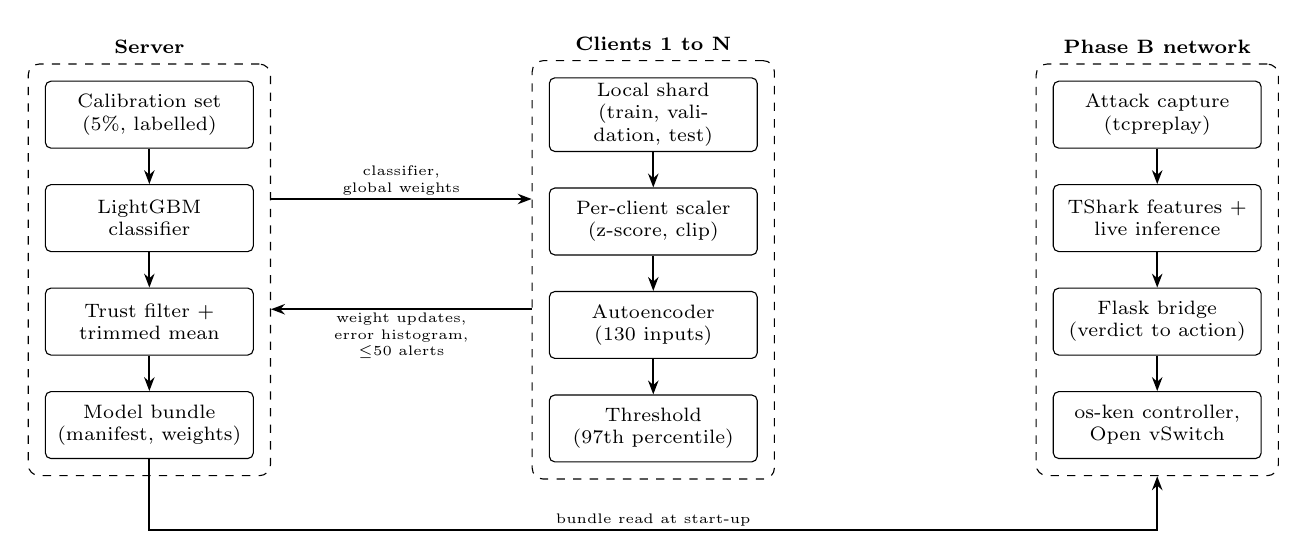
\begin{tikzpicture}[
  font=\scriptsize,
  box/.style={draw, rounded corners=2pt, align=center, minimum height=0.85cm, text width=2.5cm, inner sep=2pt},
  grp/.style={draw, dashed, rounded corners=4pt, inner sep=6pt},
  arr/.style={-{Stealth[length=5pt]}, thick},
  lab/.style={font=\tiny, align=center, fill=white, inner sep=1pt}
]
\node[box] (cal) at (0,0) {Calibration set\\(5\%, labelled)};
\node[box, below=0.45cm of cal] (lgbm) {LightGBM\\classifier};
\node[box, below=0.45cm of lgbm] (strat) {Trust filter +\\trimmed mean};
\node[box, below=0.45cm of strat] (bundle) {Model bundle\\(manifest, weights)};
\node[grp, fit=(cal)(lgbm)(strat)(bundle), label={[font=\scriptsize\bfseries]above:Server}] (server) {};

\node[box] (shard) at (6.4,0) {Local shard\\(train, validation, test)};
\node[box, below=0.45cm of shard] (scaler) {Per-client scaler\\(z-score, clip)};
\node[box, below=0.45cm of scaler] (ae) {Autoencoder\\(130 inputs)};
\node[box, below=0.45cm of ae] (thr) {Threshold\\(97th percentile)};
\node[grp, fit=(shard)(scaler)(ae)(thr), label={[font=\scriptsize\bfseries]above:Clients 1 to N}] (clients) {};

\node[box] (cap) at (12.8,0) {Attack capture\\(tcpreplay)};
\node[box, below=0.45cm of cap] (live) {TShark features +\\live inference};
\node[box, below=0.45cm of live] (flask) {Flask bridge\\(verdict to action)};
\node[box, below=0.45cm of flask] (ovs) {os-ken controller,\\Open vSwitch};
\node[grp, fit=(cap)(live)(flask)(ovs), label={[font=\scriptsize\bfseries]above:Phase B network}] (net) {};

\draw[arr] (cal) -- (lgbm);
\draw[arr] (lgbm) -- (strat);
\draw[arr] (strat) -- (bundle);
\draw[arr] (shard) -- (scaler);
\draw[arr] (scaler) -- (ae);
\draw[arr] (ae) -- (thr);
\draw[arr] (cap) -- (live);
\draw[arr] (live) -- (flask);
\draw[arr] (flask) -- (ovs);

\draw[arr] ([yshift=0.9cm]server.east) -- node[lab, above] {classifier,\\global weights} ([yshift=0.9cm]clients.west);
\draw[arr] ([yshift=-0.5cm]clients.west) -- node[lab, below] {weight updates,\\error histogram,\\$\le$50 alerts} ([yshift=-0.5cm]server.east);
\draw[arr] (bundle.south) -- ++(0,-0.9) -| node[lab, pos=0.25, above] {bundle read at start-up} (net.south);
\end{tikzpicture}}
\caption{Deployment view of FL-IDS: server, clients and the emulated network}
\label{fig:deploy}
\end{figure}

Figure~\ref{fig:hld} gives the same design as a block diagram of the two phases.
\begin{figure}[H]
\centering
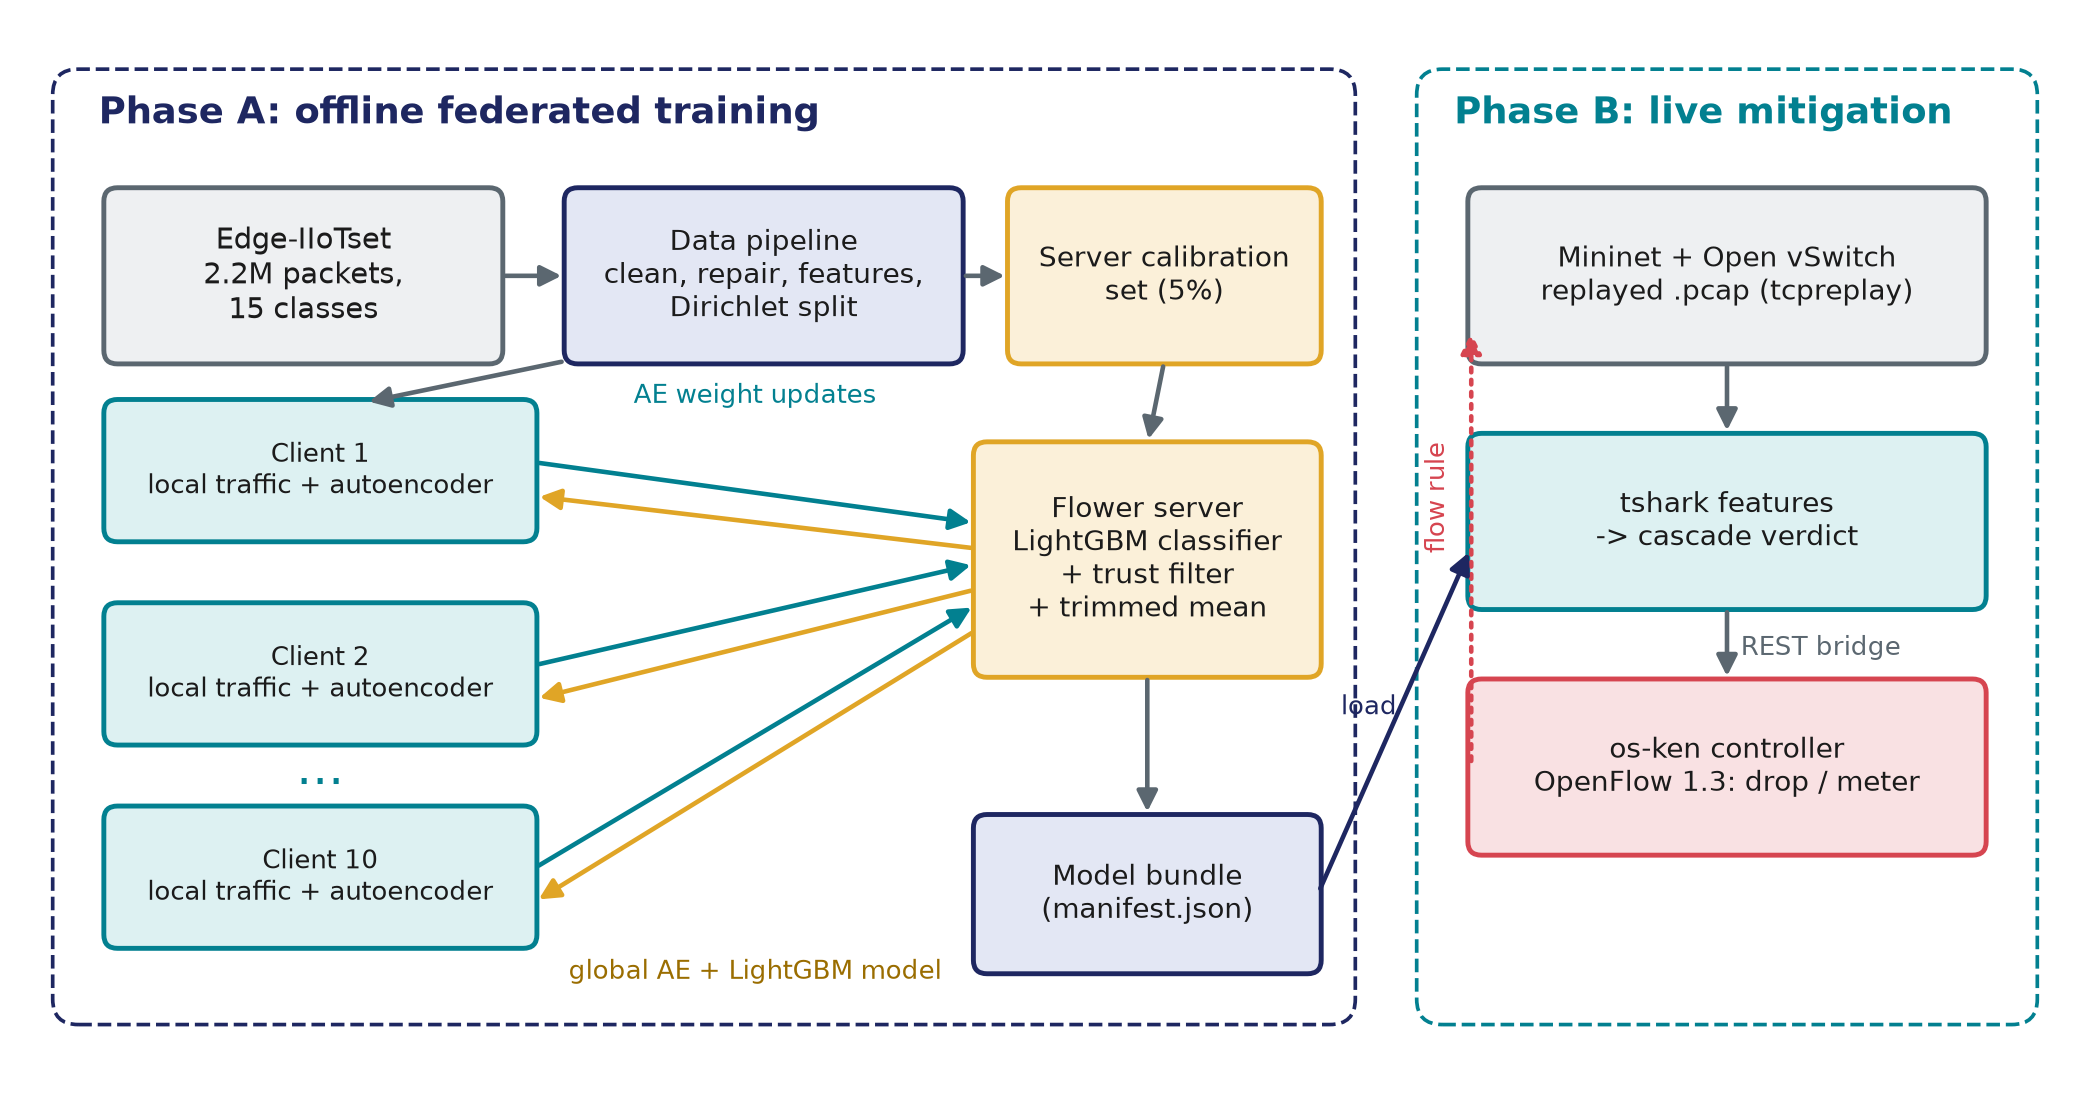
\includegraphics[width=\linewidth]{figures/high_level_design.png}
\caption{High-level design of FL-IDS}
\label{fig:hld}
\end{figure}

Four design decisions shape everything else.
\begin{enumerate}
  \item \textbf{Raw features for the classifier, normalised features for the autoencoder.} Trees split on raw values, so a client's own scaling cannot distort the shared classifier; the autoencoder needs scaled inputs and each client scales with its own statistics.
  \item \textbf{One decision rule.} The cascade rule exists in a single module and is used by the evaluation code, the dashboard and the SDN path, so the three cannot disagree.
  \item \textbf{Filtering on deltas.} The trust filter looks at each client's change to the weights, not at the weights, because honest weights differ a lot between non-IID clients but their updates point the same way.
  \item \textbf{A self-describing bundle.} Phase B rebuilds everything from the bundle's manifest, never from the current configuration, and refuses a bundle whose saved thresholds do not match the saved weights.
\end{enumerate}

\section{Module/Component Design}
The code is a Python package, \texttt{fl\_ids}, with one sub-package per component. Table~\ref{tab:modules} lists them.
\begin{table}[H]
\centering
\scriptsize
\renewcommand{\arraystretch}{1.2}
\begin{tabular}{|>{\raggedright\arraybackslash}p{2.6cm}|>{\raggedright\arraybackslash}p{3.9cm}|>{\raggedright\arraybackslash}p{6.4cm}|}
\hline
\textbf{Sub-package} & \textbf{Modules} & \textbf{Responsibility} \\ \hline
\texttt{data} & \texttt{pipeline}, \texttt{repair}, \texttt{features}, \texttt{sampling}, \texttt{synthetic} & Cleaning, MITM repair, one-hot encoding, service-port, content and flow features, connection-grouped splitting and the Dirichlet partition; a synthetic generator for tests \\ \hline
\texttt{models} & \texttt{boosting}, \texttt{boosting\_update}, \texttt{autoencoder}, \texttt{cascade}, \texttt{dl\_classifier} & First-stage classifier and its incremental update, the autoencoder, the shared cascade rule, and the deep-learning baseline \\ \hline
\texttt{fl} & \texttt{client}, \texttt{server}, \texttt{strategy}, \texttt{launch}, \texttt{data\_io} & Flower client and server, the custom strategy, starting the processes, loading each client's shard \\ \hline
\texttt{robustness} & \texttt{trust\_filter}, \texttt{aggregation}, \texttt{attackers} & Cosine/MAD/EMA filter, clipping and trimmed mean, and the sign-flip and stealth test attackers \\ \hline
\texttt{sdn} & \texttt{topology}, \texttt{controller}, \texttt{bridge}, \texttt{feature\_extraction}, \texttt{live\_inference}, \texttt{demo\_io} & Mininet topology, os-ken OpenFlow 1.3 controller, Flask bridge, TShark-based feature extraction and per-host scoring \\ \hline
\texttt{orchestration} & \texttt{phase\_a}, \texttt{phase\_b}, \texttt{artifacts} & Phase A and Phase B entry points; saving and loading the model bundle \\ \hline
\texttt{eval} & 18 modules, including \texttt{ablation}, \texttt{poisoning\_sweep}, \texttt{zero\_day}, \texttt{adaptive\_attack}, \texttt{pruning}, \texttt{metrics} & Every experiment in Chapter~\ref{chap:results} and the metrics they share \\ \hline
\texttt{dashboard} & \texttt{app}, \texttt{data} & Streamlit view of training and mitigation state \\ \hline
\texttt{utils} & \texttt{config}, \texttt{journey}, \texttt{logging\_setup} & Configuration loading, stage timing (the ``journey''), logging \\ \hline
\end{tabular}
\caption{Packages and modules of FL-IDS}
\label{tab:modules}
\end{table}
Outside the package, \texttt{configs/} holds one YAML file per experiment, \texttt{tools/} holds the latency benchmark and similar one-off tools, and \texttt{tests/} holds the automated tests.

\section{Detailed Design}
\subsection{One federated round}
Figure~\ref{fig:round} (Chapter~\ref{chap:method}) shows the arithmetic; Figure~\ref{fig:seq} shows the order of messages. The server never sees a packet: it receives weights, a 50-bin histogram of reconstruction errors, and every third round at most 50 confirmed alerts per surviving client.
\begin{figure}[H]
\centering
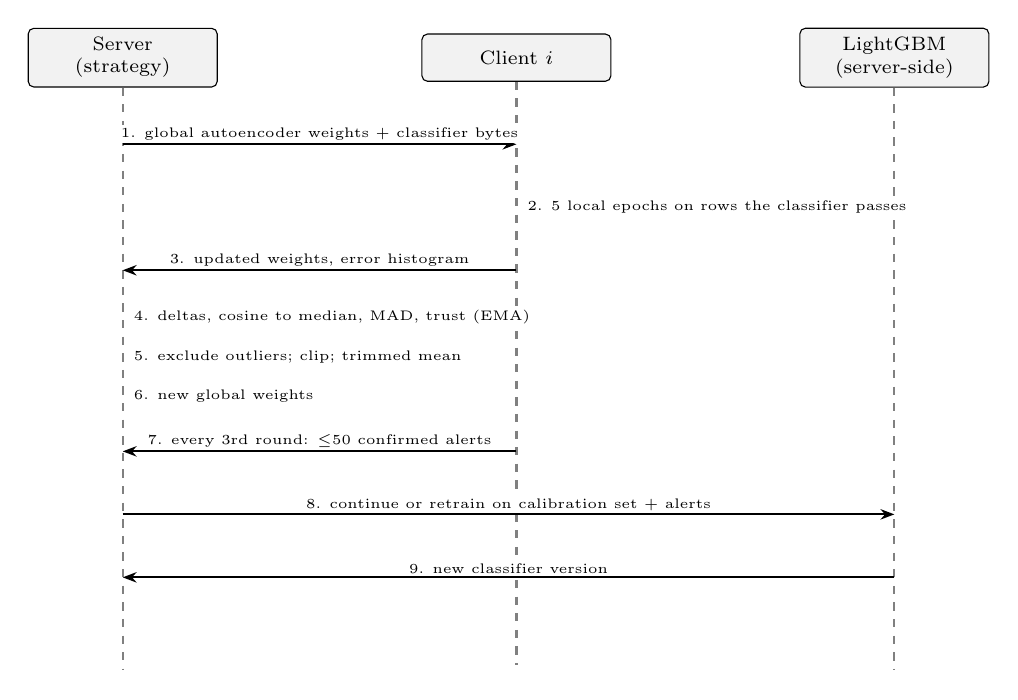
\begin{tikzpicture}[
  font=\scriptsize,
  life/.style={thick, dashed, gray},
  head/.style={draw, rounded corners=2pt, minimum width=2.4cm, minimum height=0.6cm, align=center, fill=gray!10},
  msg/.style={-{Stealth[length=5pt]}, thick},
  note/.style={font=\tiny, fill=white, inner sep=1pt}
]
\node[head] (S) at (0,0) {Server\\(strategy)};
\node[head] (C) at (5,0) {Client $i$};
\node[head] (B) at (9.8,0) {LightGBM\\(server-side)};
\draw[life] (S.south) -- ++(0,-7.4);
\draw[life] (C.south) -- ++(0,-7.4);
\draw[life] (B.south) -- ++(0,-7.4);
\draw[msg] (0,-1.1) -- node[note, above] {1. global autoencoder weights + classifier bytes} (5,-1.1);
\node[note, anchor=west] at (5.1,-1.9) {2. 5 local epochs on rows the classifier passes};
\draw[msg] (5,-2.7) -- node[note, above] {3. updated weights, error histogram} (0,-2.7);
\node[note, anchor=west] at (0.1,-3.3) {4. deltas, cosine to median, MAD, trust (EMA)};
\node[note, anchor=west] at (0.1,-3.8) {5. exclude outliers; clip; trimmed mean};
\node[note, anchor=west] at (0.1,-4.3) {6. new global weights};
\draw[msg] (5,-5.0) -- node[note, above] {7. every 3rd round: $\le$50 confirmed alerts} (0,-5.0);
\draw[msg] (0,-5.8) -- node[note, above] {8. continue or retrain on calibration set + alerts} (9.8,-5.8);
\draw[msg] (9.8,-6.6) -- node[note, above] {9. new classifier version} (0,-6.6);
\end{tikzpicture}
\caption{Order of messages in one federated round}
\label{fig:seq}
\end{figure}

\subsection{Cascade decision}
\begin{enumerate}
  \item The LightGBM classifier returns a class and its probability $p$.
  \item If the class is an attack and $p\ge0.7$ the label is final (the classifier's confidence is reported).
  \item Otherwise the autoencoder's reconstruction error $e$ is compared with the client's threshold $\tau_i$; $e>\tau_i$ gives \emph{anomalous}, with confidence $\mathrm{clip}(e/\tau_i-1,0,1)$.
  \item Anything else is benign.
\end{enumerate}
The module returns the label, the confidence and the stage that decided, which the bridge and the dashboard reuse. Figure~\ref{fig:cascade} (Chapter~\ref{chap:method}) is the flow chart of this rule.

\subsection{Trust filter and aggregation}
The filter is a pure function of the round's deltas and the previous trust scores: it returns which clients survive, why each excluded client was excluded (\texttt{mad\_outlier}, \texttt{opposes\_consensus} or \texttt{low\_trust}) and the new trust scores. Aggregation is a second pure function that takes the survivors' deltas, clips them and applies the trimmed mean. Keeping both free of Flower types made them testable on small arrays, and \texttt{TrustFilteredStrategy} only glues them to Flower's \texttt{aggregate\_fit}. If no client survives, the round is skipped.

\subsection{Phase B: from capture to rule}
\begin{enumerate}
  \item Mininet starts one host per federated client on one Open vSwitch switch; the os-ken controller connects over OpenFlow~1.3.
  \item \texttt{tcpreplay} sends a dataset capture from one host.
  \item TShark extracts the dataset's 61 fields; the same feature code as in training derives the 130 features.
  \item Each row is scored with that host's scaler and threshold; the most frequent non-benign label is the host's verdict, with its confidence and deciding stage.
  \item The Flask bridge receives \{device, classification, confidence, stage\}. Confidence $\ge0.85$ gives \emph{block}, $\ge0.5$ \emph{rate-limit}, otherwise \emph{allow}.
  \item The controller installs \texttt{priority=100,ip,nw\_src=}\emph{attacker}\texttt{ actions=drop} (or a meter), and the result is read back from the switch's flow table and saved with the verdict.
\end{enumerate}
Mininet needs root rights; it is started through a single permitted command whose parameters travel through a fixed file, so no other privileged command is exposed.

\subsection{Classes and interfaces that matter}
\begin{itemize}
  \item \textbf{Configuration}: a set of dataclasses (data, boosting, autoencoder, cascade and so on) loaded from YAML, so every value in a run is recorded with the run (\texttt{config.yaml} is copied into each run directory).
  \item \textbf{Bundle}: a loader that validates before use (Section~\ref{sec:datadesign}).
  \item \textbf{Cascade}: \texttt{flag\_attacks(mode, \ldots)} with the modes \texttt{boosting\_only}, \texttt{autoencoder\_only} and \texttt{cascade}, which is how the ablation and the latency benchmark call the same code path.
  \item \textbf{Journey}: a stage timer that records how long each step of a run took (loading and cleaning, bootstrap classifier and partition, federated training, threshold calibration, evaluation, saving the bundle).
\end{itemize}

\section{Data Design}\label{sec:datadesign}
\subsection{Dataset and splits}
Figure~\ref{fig:datasplit} shows how the dataset is divided. Rows are grouped into connections first; a connection is never divided.
\begin{figure}[H]
\centering
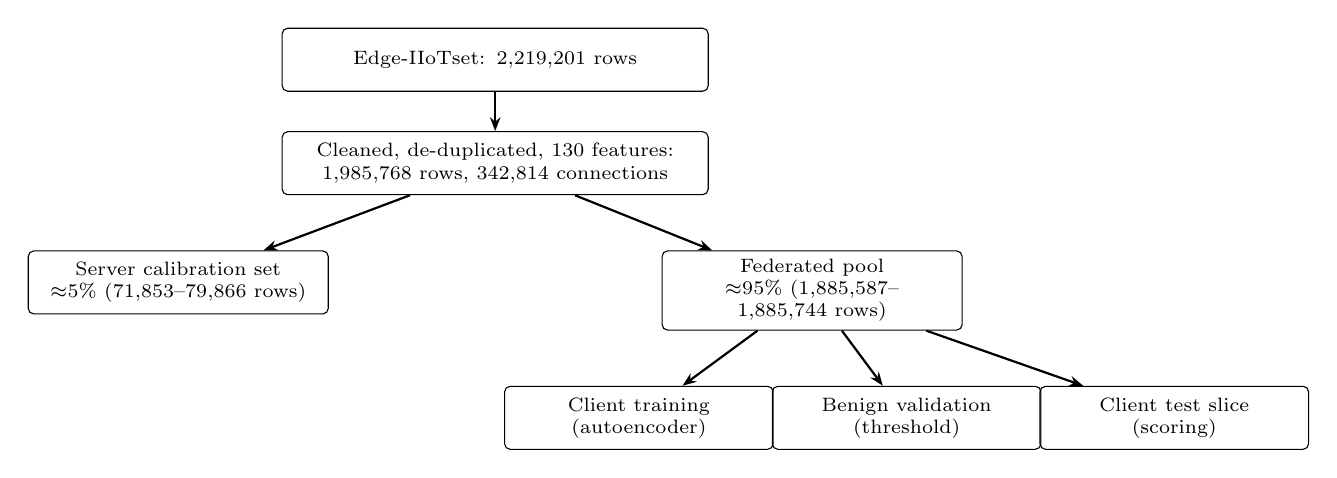
\begin{tikzpicture}[
  font=\scriptsize,
  box/.style={draw, rounded corners=2pt, align=center, minimum height=0.8cm, inner sep=3pt},
  arr/.style={-{Stealth[length=5pt]}, thick}
]
\node[box, text width=5.2cm] (raw) at (0,0) {Edge-IIoTset: 2{,}219{,}201 rows};
\node[box, text width=5.2cm, below=0.5cm of raw] (clean) {Cleaned, de-duplicated, 130 features:\\1{,}985{,}768 rows, 342{,}814 connections};
\node[box, text width=3.6cm, below left=0.7cm and -0.6cm of clean] (cal) {Server calibration set\\$\approx$5\% (71{,}853--79{,}866 rows)};
\node[box, text width=3.6cm, below right=0.7cm and -0.6cm of clean] (pool) {Federated pool\\$\approx$95\% (1{,}885{,}587--1{,}885{,}744 rows)};
\node[box, text width=3.2cm, below=0.7cm of pool, xshift=-2.2cm] (tr) {Client training\\(autoencoder)};
\node[box, text width=3.2cm, below=0.7cm of pool, xshift=1.2cm] (va) {Benign validation\\(threshold)};
\node[box, text width=3.2cm, below=0.7cm of pool, xshift=4.6cm] (te) {Client test slice\\(scoring)};
\draw[arr] (raw) -- (clean);
\draw[arr] (clean) -- (cal);
\draw[arr] (clean) -- (pool);
\draw[arr] (pool) -- (tr);
\draw[arr] (pool) -- (va);
\draw[arr] (pool) -- (te);
\end{tikzpicture}
\caption{How the dataset is divided; every connection goes to exactly one box}
\label{fig:datasplit}
\end{figure}
The pool is divided among $N$ clients with a Dirichlet($\alpha=0.3$) label skew, so some clients see almost no benign traffic (up to three of 20 clients had no benign validation rows in the main runs).

\subsection{Files written by a run}
\begin{table}[H]
\centering
\scriptsize
\renewcommand{\arraystretch}{1.2}
\begin{tabular}{|>{\raggedright\arraybackslash}p{4.6cm}|>{\raggedright\arraybackslash}p{8.4cm}|}
\hline
\textbf{File} & \textbf{Contents} \\ \hline
\texttt{boosting\_model.txt} & The LightGBM model in text form \\ \hline
\texttt{autoencoder\_weights.npz} & Final global autoencoder weights \\ \hline
\texttt{client\_normalization.npz} & Each client's mean, scale and threshold \\ \hline
\texttt{manifest.json} & Class names, the 130 feature names, input size, autoencoder shape, cascade settings, clip value, thresholds, held-out metrics, training summary (rounds, trust scores, survivors, classifier updates), seed, data set name, creation time and git commit \\ \hline
\texttt{journey.json} & Seconds spent in each stage of the run \\ \hline
\texttt{runs/.../phase\_a/} & Per-client logs and arrays, calibration arrays and the configuration used \\ \hline
\texttt{runs/.../phase\_b/} & Topology, bridge and controller logs, and \texttt{phase\_b\_result.json} with the verdict, the action and the flow table read back \\ \hline
\texttt{results/*.json} & One file per experiment (for example the latency benchmark) \\ \hline
\end{tabular}
\caption{Files that make up a model bundle and a run record}
\label{tab:files}
\end{table}

\subsection{Record layout}
A record is a vector of 130 numeric features. The first 91 are the dataset's own fields after dropping 16 columns and one-hot encoding seven nominal ones; one is the service port, 18 describe payload content and 20 describe the flow the packet belongs to (Section~\ref{sec:newfeat}). Class labels are stored as indices into the manifest's \texttt{class\_names} list, with Normal as the benign class. Identifiers (IP addresses, absolute time, ephemeral ports) are used only to group packets into flows and connections and are never stored as features.

\subsection{Bundle validation}
On load, Phase B recomputes every client's threshold from the saved weights and checks that it equals the saved threshold and rejects the bundle if they differ. This catches a bundle assembled from two different runs.

\chapter{Methodology}\label{chap:method}
FL-IDS runs in two phases. \textbf{Phase A} prepares the data, trains the LightGBM classifier, trains the autoencoder over 20 federated rounds with the trust filter, evaluates everything, and saves a model bundle. \textbf{Phase B} loads that bundle, classifies replayed attack traffic on an emulated network and turns the verdict into an OpenFlow rule. Figure~\ref{fig:hld} shows the overall design.

\section{Tools and Techniques}
\begin{itemize}
  \item \textbf{LightGBM}~\cite{ke2017lightgbm}: histogram-based gradient-boosted decision trees, used as the first-stage multi-class classifier. Trees work directly on raw feature values, so each client's local normalisation cannot distort the classifier's split thresholds.
  \item \textbf{Autoencoder (PyTorch)}: a dense network $130\rightarrow32\rightarrow16\rightarrow8\rightarrow16\rightarrow32\rightarrow130$ with ReLU activations and a linear output, 9{,}834 parameters in total (7{,}299 with the original 91 features). It learns to reconstruct benign traffic, so a high reconstruction error indicates unusual traffic.
  \item \textbf{Flower}: the federated learning framework. A custom strategy, \texttt{TrustFiltered\-Strategy} (a subclass of FedAvg), implements the trust filter and trimmed-mean aggregation.
  \item \textbf{Cosine similarity, median absolute deviation (MAD) and exponential moving average (EMA)}: the statistics used by the trust filter.
  \item \textbf{Mininet, Open vSwitch, os-ken}: network emulation, the software switch, and the OpenFlow~1.3 controller (os-ken is the maintained fork of Ryu).
  \item \textbf{TShark and tcpreplay}: extracting the dataset's fields from live packets, and replaying captures into the emulated network.
  \item \textbf{Streamlit}: the live dashboard.
\end{itemize}

\section{Data Set with Explanation}\label{sec:dataset}
\textbf{Edge-IIoTset}~\cite{ferrag2022edge} was generated on a seven-layer IoT/IIoT testbed (cloud, network functions virtualisation, blockchain, fog, SDN, edge and IoT/IIoT perception layers) with more than ten kinds of sensors, including temperature, humidity, water level, pH, soil moisture, heart rate and flame sensors. They communicate over MQTT and Modbus/TCP. The authors' ML-ready file, \texttt{DNN-EdgeIIoT-dataset.csv}, has 2{,}219{,}201 rows and 63 columns: 61 packet-level fields extracted with tshark, plus \texttt{Attack\_label} and \texttt{Attack\_type}. The 24 per-device and per-attack \texttt{.pcap} captures are also used, for Phase B replay and for repairing corrupted rows.

There are 15 classes: Normal and 14 attacks in five groups. Table~\ref{tab:classes} gives the class sizes after cleaning (current code, before the new features are added).

\begin{table}[H]
\centering
\renewcommand{\arraystretch}{1.15}
\begin{tabular}{|l|l|r|r|}
\hline
\textbf{Group} & \textbf{Class} & \textbf{Rows} & \textbf{\%} \\ \hline
-- & Normal & 1{,}363{,}998 & 71.42 \\ \hline
DoS/DDoS & DDoS\_UDP & 121{,}567 & 6.37 \\
 & DDoS\_ICMP & 67{,}939 & 3.56 \\
 & DDoS\_TCP & 50{,}062 & 2.62 \\
 & DDoS\_HTTP & 48{,}544 & 2.54 \\ \hline
Injection & SQL\_injection & 50{,}826 & 2.66 \\
 & Uploading & 36{,}807 & 1.93 \\
 & XSS & 15{,}066 & 0.79 \\ \hline
Information gathering & Vulnerability\_scanner & 50{,}026 & 2.62 \\
 & Port\_Scanning & 19{,}977 & 1.05 \\
 & Fingerprinting & 853 & 0.04 \\ \hline
Malware & Password & 49{,}933 & 2.61 \\
 & Backdoor & 24{,}026 & 1.26 \\
 & Ransomware & 9{,}689 & 0.51 \\ \hline
Man-in-the-middle & MITM & 406 & 0.02 \\ \hline
\multicolumn{2}{|l|}{\textbf{Total}} & \textbf{1{,}909{,}719} & \\ \hline
\end{tabular}
\caption{Class distribution after cleaning (91 base features)}
\label{tab:classes}
\end{table}

\subsection{Data-quality problems found and fixed}\label{sec:dataquality}
\begin{enumerate}
  \item \textbf{Placeholder label leak.} In the categorical columns, the ``field does not apply'' value is written as \texttt{0} in some source captures and \texttt{0.0} in others, and the spelling follows the label. In \texttt{mqtt.topic}, \texttt{mqtt.conack.flags}, \texttt{mqtt.protoname} and \texttt{dns.qry.name.len}, every Normal row uses \texttt{0} and every attack row \texttt{0.0}. After one-hot encoding, the single column \texttt{mqtt.topic\_0.0} separates benign from attack with an AUROC of 1.0. Both spellings are mapped to \texttt{0} before encoding, after which the strongest single feature has an AUROC of about 0.71. A test guards that no single feature exceeds 0.9. We found this independently, but Galal~\cite{galal2026provenance} reported the same serialisation artefact first, so it is not claimed as a contribution of this project.
  \item \textbf{Column-shifted MITM rows.} In the authors' MITM rows, values sit under the wrong column names (for example, their \texttt{tcp.seq} is really \texttt{udp.time\_delta}, with 1.000 agreement). These rows are replaced by re-extracting the authors' own MITM capture with the same field list (1{,}214 rows replaced by 1{,}229). Galal~\cite{galal2026provenance} keeps these rows as released and does not report the shift; we found no other report of it.
  \item \textbf{TShark version drift.} Newer tshark prints booleans as \texttt{True}/\texttt{False} and shortens hexadecimal values. Without a fix, this silently zeroed \texttt{tcp.flags.ack} on every live packet in Phase B. Live extraction maps both back to the authors' format.
\end{enumerate}

\subsection{Preprocessing}
Sixteen columns are dropped, following the dataset authors' recipe: identifiers, timestamps, raw payloads and ports, plus \texttt{Attack\_label}, which is fully determined by \texttt{Attack\_type}. Seven nominal columns are one-hot encoded, giving \textbf{91 base features}. Exact duplicate rows are removed (309{,}497 rows), leaving 1{,}909{,}719 rows.

\subsection{New features for the classifier}\label{sec:newfeat}
Profiling the dropped columns explained why the application-layer attacks were hard to classify. In the SQL\_injection, XSS, Uploading and Password classes, only 5--17\% of packets carry any HTTP content. The rest are content-free TCP handshake and acknowledgement packets to port~80 on the same web server, which look the same whichever attack produced them. Three groups of features were therefore added. IP addresses, absolute time and ephemeral client ports are \emph{never} used as features, because each of them identifies the capture file and hence the label.
\begin{enumerate}
  \item \textbf{Service port (1 feature):} the server side of a connection, $\min(\text{ports} < 32768)$, or $-1$ if there is none (for example ICMP or ARP).
  \item \textbf{Content features (18):} decoded payload length, byte entropy, printable fraction, HTTP request flag, HTTP status code, header count, \texttt{X-} header count, URI length, parameter count, percent-encoding count, file-data length, special-character count, and counts of six generic attack-signature keyword groups (SQL, script/XSS, upload, authentication, traversal/command, scanner tool names).
  \item \textbf{Flow features (20):} packets are grouped into flows by (IP pair, protocol, port pair) in capture order. A new flow starts after a 60\,s idle gap or once a flow has been active for 120\,s, CICFlowMeter's default active timeout~\cite{sharafaldin2018cicids}. Every packet in a flow receives the flow's packet count, duration, packet rate, payload sum/maximum/non-zero share, HTTP request count, maximum status code, SYN, FIN and RST counts, maximum entropy, maximum URI length and keyword totals. IP addresses and times are used only to group packets, never as features.
\end{enumerate}
With all three groups there are 130 features and 1{,}985{,}768 unique rows.

\textbf{Class split of the final data.} After the new features are added and duplicates are removed, 1{,}985{,}768 unique rows remain; Table~\ref{tab:classes130} gives the class sizes (the 342{,}814 connections they form are what the splits keep whole). Table~\ref{tab:classes} above was counted on the 91 base features before the last cleaning step and is kept to show what changed.
\begin{table}[H]
\centering
\small
\renewcommand{\arraystretch}{1.15}
\begin{tabular}{|l|l|r|r|}
\hline
\textbf{Group} & \textbf{Class} & \textbf{Rows} & \textbf{\%} \\ \hline
-- & Normal & 1{,}436{,}597 & 72.34 \\ \hline
DoS/DDoS & DDoS\_UDP & 121{,}567 & 6.12 \\ \hline
DoS/DDoS & DDoS\_ICMP & 68{,}758 & 3.46 \\ \hline
DoS/DDoS & DDoS\_TCP & 50{,}062 & 2.52 \\ \hline
DoS/DDoS & DDoS\_HTTP & 49{,}768 & 2.51 \\ \hline
Injection & SQL\_injection & 50{,}981 & 2.57 \\ \hline
Injection & Uploading & 37{,}243 & 1.88 \\ \hline
Injection & XSS & 15{,}172 & 0.76 \\ \hline
Information gathering & Vulnerability\_scanner & 50{,}044 & 2.52 \\ \hline
Information gathering & Port\_Scanning & 20{,}213 & 1.02 \\ \hline
Information gathering & Fingerprinting & 872 & 0.04 \\ \hline
Malware & Password & 50{,}033 & 2.52 \\ \hline
Malware & Backdoor & 24{,}167 & 1.22 \\ \hline
Malware & Ransomware & 9{,}885 & 0.50 \\ \hline
Man-in-the-middle & MITM & 406 & 0.02 \\ \hline
\textbf{Total} & & \textbf{1{,}985{,}768} & \textbf{100.00} \\ \hline
\end{tabular}
\caption{Class distribution of the final data (130 features)}
\label{tab:classes130}
\end{table}

\section{Flowchart of Methodology from Start to End}
Figure~\ref{fig:flow} shows the complete sequence of steps, from loading the dataset to verifying the mitigation rule.
\begin{figure}[H]
\centering
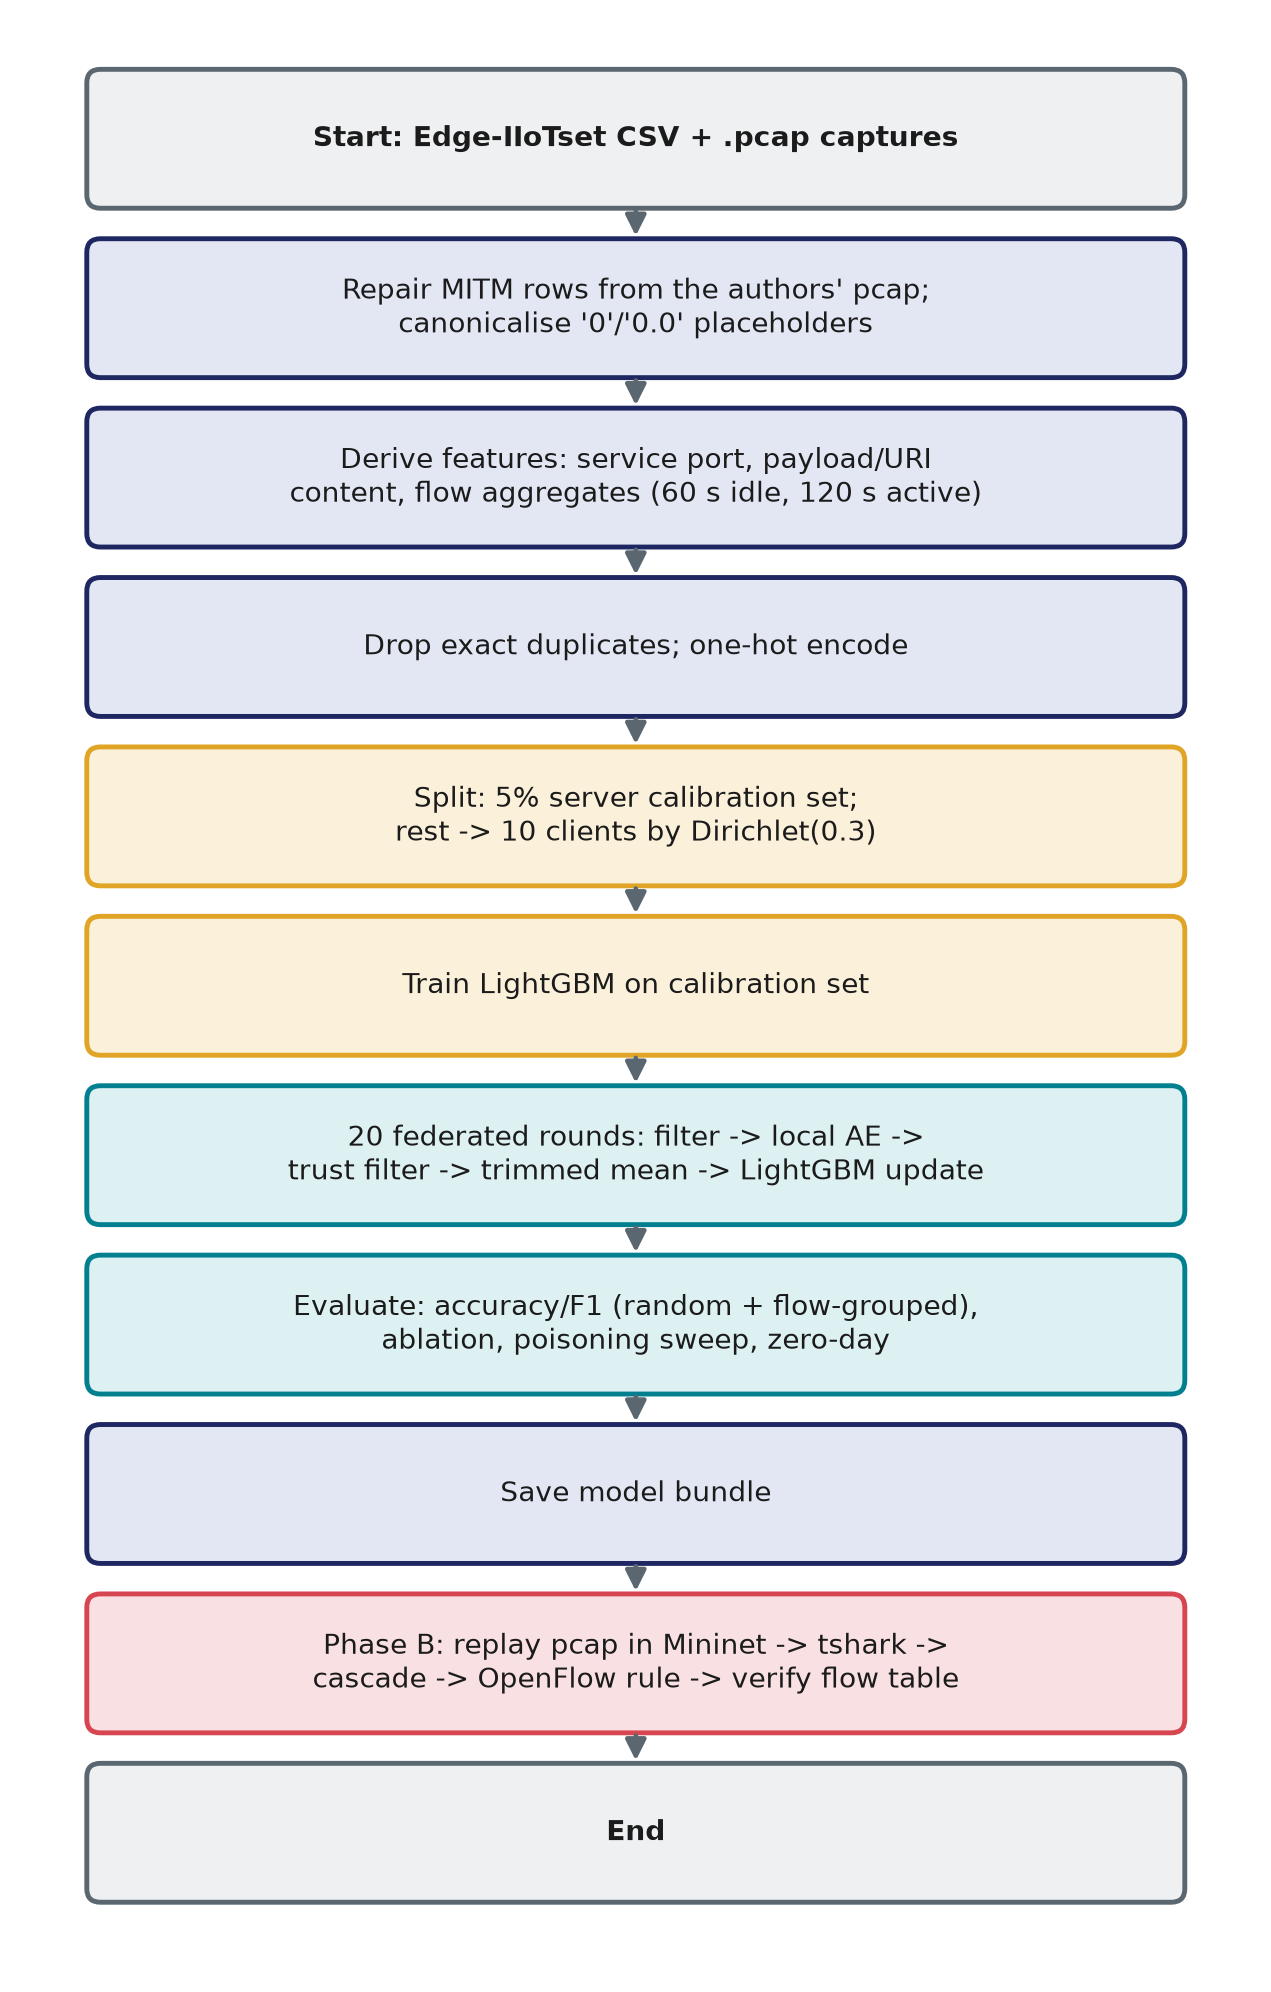
\includegraphics[width=0.62\linewidth]{figures/methodology_flowchart.png}
\caption{Flow chart of the methodology}
\label{fig:flow}
\end{figure}

\section{Explanation of Methodology in Detail with Equations and Formulae}

\subsection{How much data each part uses}
Every packet of the dataset is cleaned and given the new features (2{,}219{,}216 rows, 1{,}985{,}768 unique after de-duplication). How many of them each model trains on differs, and Table~\ref{tab:datascale} lists it. The classifier that meets the accuracy target is trained on most of the data. The federated system was first run on a pool capped at 60{,}000 rows, to keep the roughly 150 evaluation runs practical; the main federated results (Section~\ref{sec:fullpool}) use the whole pool.
\begin{table}[H]
\centering
\small
\renewcommand{\arraystretch}{1.2}
\begin{tabular}{|>{\raggedright\arraybackslash}p{4.4cm}|>{\raggedright\arraybackslash}p{4.7cm}|>{\raggedright\arraybackslash}p{4.7cm}|}
\hline
\textbf{Part} & \textbf{Trained on} & \textbf{Evaluated on} \\ \hline
Final classifier (accuracy target) & 1{,}429{,}825 rows (72\%), plus 158{,}870 for early stopping (8\%) & 397{,}073 unseen rows (20\%); whole connections held out \\ \hline
Same classifier, 5\% share only & 89{,}359 rows, plus 9{,}929 for early stopping & the same 397{,}073 rows \\ \hline
Federated: server bootstrap classifier & 79{,}430 rows (calibration set) & 19{,}858 rows held back \\ \hline
Federated, earlier 60k pool: client autoencoders & 45{,}474 rows across 10 clients (736 to 11{,}549 each), plus 5{,}530 benign rows for thresholds & 8{,}996 client test rows \\ \hline
Federated, full pool: server bootstrap classifier & 71{,}853 to 79{,}866 rows (calibration set, whole connections) & a part held back for scoring boosting versions \\ \hline
Federated, full pool: client autoencoders & the 1{,}885{,}587 to 1{,}885{,}744 pool rows across 10 or 20 clients, split by connection (training, benign-validation and test slices) & 283{,}090 to 295{,}566 client test rows \\ \hline
\end{tabular}
\caption{Training and evaluation rows for each part (130 features, seed 42)}
\label{tab:datascale}
\end{table}
The 5\%-only row shows that the federated bootstrap loses little from its smaller training set: 99.7\% accuracy and 0.979 macro F1 on the same 397{,}073 test rows, against 0.983 for the full classifier.

\subsection{Non-IID partition and per-client normalisation}
A stratified 5\% of the rows is held on the server as the calibration set. The remaining federated pool (all of it in the main runs; subsampled to 60{,}000 rows in the earlier comparison runs) is split across $N=10$ clients. For each class $k$ a proportion vector is drawn,
\begin{equation}
  \mathbf{p}_k \sim \mathrm{Dir}(\alpha\mathbf{1}_N), \qquad \alpha = 0.3,
\end{equation}
and the class's rows are divided in those proportions~\cite{hsu2019noniid}. Smaller $\alpha$ gives more skew. In the full-pool runs the unit that is divided is the connection, not the row: each connection goes to one client, and within a client it goes to exactly one of the training, benign-validation and test slices, so no test packet has a sibling from the same connection in training. Each client keeps 15\% as a test slice and 15\% of its benign remainder as a benign validation slice. For the autoencoder only, client $i$ standardises features with its own training mean $\mu_i$ and standard deviation $\sigma_i$, clipped at $\pm10$:
\begin{equation}
  \tilde{x} = \mathrm{clip}\!\left(\frac{x-\mu_i}{\sigma_i},\,-10,\,10\right).
\end{equation}
The clip is needed because a counter feature can barely vary inside one skewed shard. Without it, one client's benign validation loss stayed near 400 for 20 rounds; with it, the loss fell to 0.0146.

\subsection{Stage 1: LightGBM classifier}
LightGBM builds an additive model of $T$ trees per class, $F_k(\mathbf{x}) = \sum_{t=1}^{T} f_{t,k}(\mathbf{x})$, with class probabilities
\begin{equation}
  P(y=k\mid\mathbf{x}) = \frac{e^{F_k(\mathbf{x})}}{\sum_{j=1}^{15} e^{F_j(\mathbf{x})}},
\end{equation}
trained by minimising the weighted multi-class log loss
\begin{equation}
  \mathcal{L} = -\frac{1}{\sum_n w_n}\sum_{n} w_{n}\,\log P(y=y_n\mid\mathbf{x}_n) + \lambda_2 \sum_{t}\lVert \mathbf{v}_t\rVert^2 ,
\end{equation}
where $\mathbf{v}_t$ are leaf values and $\lambda_2 = 1$. The sample weight $w_n$ is a square-root inverse class frequency, recomputed for every training set (the bootstrap and each incremental update),
\begin{equation}
  w_n = \sqrt{\frac{\max_j N_j}{N_{y_n}}},
\end{equation}
so a rare class such as Fingerprinting counts more without being blown up the way full inverse-frequency weights would. In the federated pipeline the classifier uses 300 rounds, learning rate 0.05 and 31 leaves, trained deterministically on one thread so runs are reproducible. The stand-alone accuracy experiments of Section~\ref{sec:clfacc} used 63 leaves, learning rate 0.1, feature and bagging fractions of 0.8, and early stopping after 50 rounds without improvement on a 10\% validation split.

\subsection{Stage 2: autoencoder and threshold}
Each client trains the autoencoder $g_\theta$ on the rows the current classifier passes (predicted Normal, or an attack with probability below 0.7). It minimises the mean squared reconstruction error
\begin{equation}
  e(\mathbf{x}) = \frac{1}{d}\sum_{j=1}^{d}\big(\tilde{x}_j - g_\theta(\tilde{\mathbf{x}})_j\big)^2
\end{equation}
with Adam (learning rate $10^{-3}$, 5 local epochs, batch size 64). The client's threshold is recomputed every round as the 97th percentile of $e$ on its benign validation slice, $\tau_i = Q_{0.97}\{e(\mathbf{x}) : \mathbf{x}\in V_i\}$.

\subsection{Cascade decision rule}
Figure~\ref{fig:cascade} shows the shared decision rule. With $\hat{k}=\arg\max_k P(k\mid\mathbf{x})$ and $p = P(\hat{k}\mid\mathbf{x})$:
\begin{equation}
\text{label}(\mathbf{x}) =
\begin{cases}
  \hat{k} & \text{if } \hat{k}\neq\text{Normal and } p \geq 0.7,\\
  \text{anomalous} & \text{else if } e(\mathbf{x}) > \tau_i,\\
  \text{benign} & \text{otherwise,}
\end{cases}
\end{equation}
with confidence $p$ for a known attack and $\mathrm{clip}(e/\tau_i - 1,\,0,\,1)$ for an anomaly.
\begin{figure}[H]
\centering
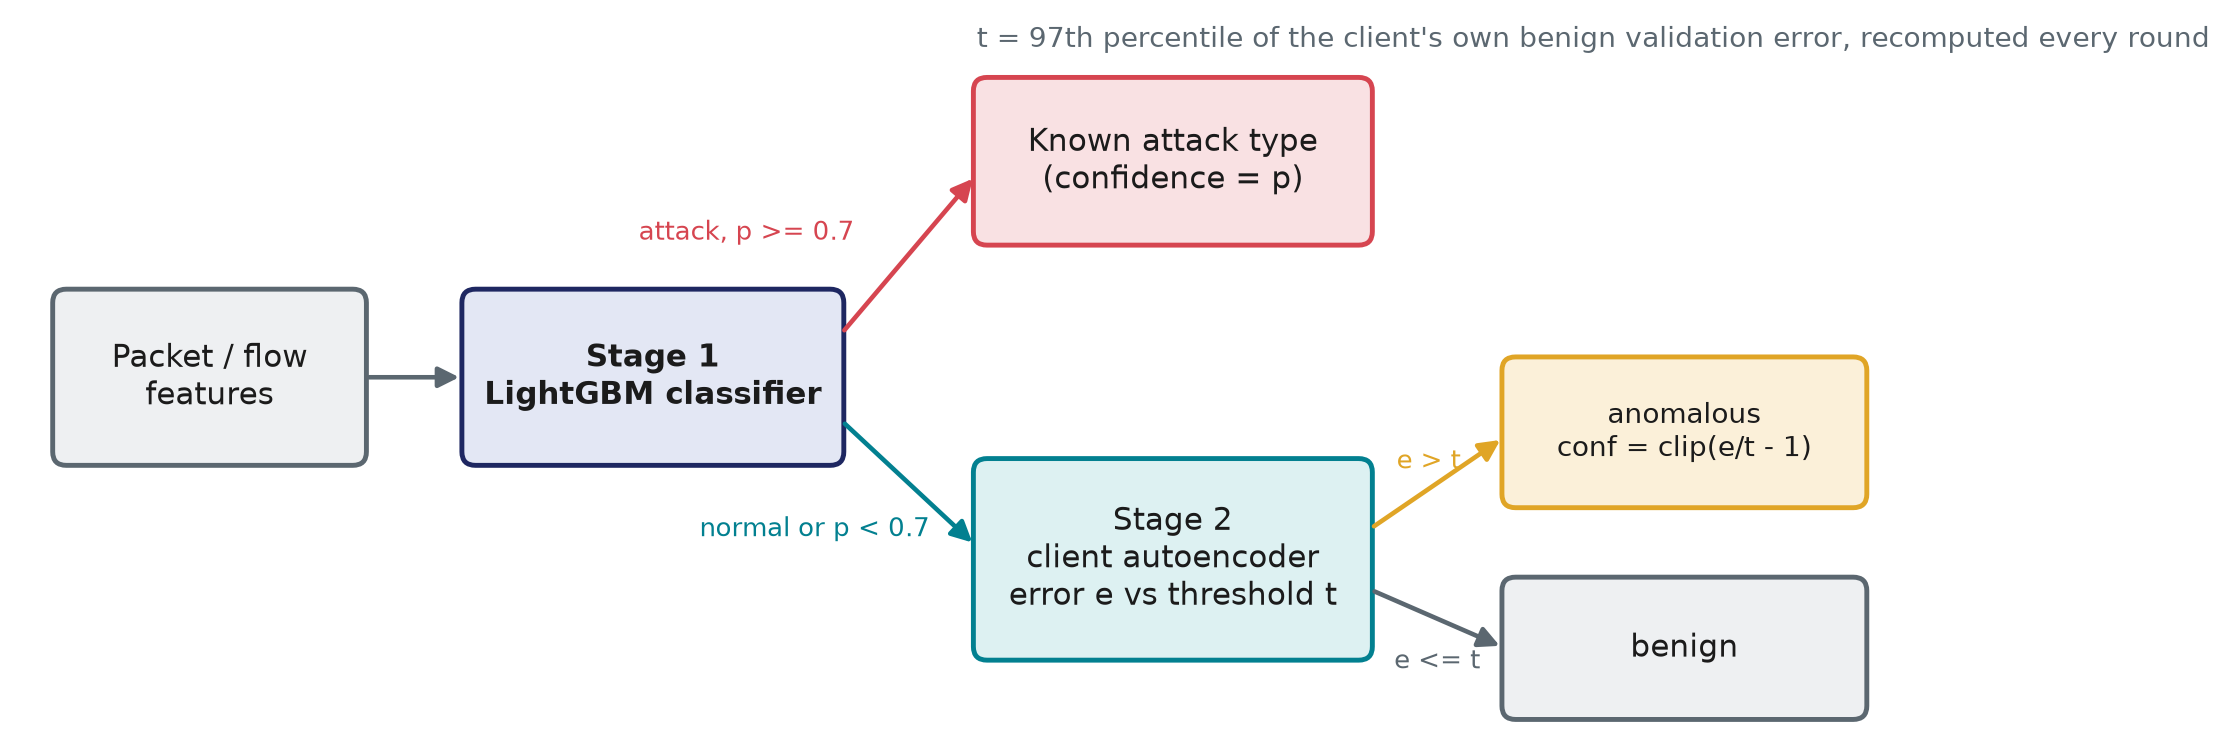
\includegraphics[width=0.92\linewidth]{figures/cascade_rule.png}
\caption{Two-stage cascade decision rule}
\label{fig:cascade}
\end{figure}

\subsection{Trust filter and robust aggregation}
Let $\mathbf{w}^{(r)}$ be the global weights at the start of round $r$ and $\mathbf{w}_i$ client $i$'s weights after local training. The filter works on \emph{deltas} $\Delta_i = \mathbf{w}_i - \mathbf{w}^{(r)}$. The reference direction is the coordinate-wise median $\mathbf{m} = \mathrm{median}_i(\Delta_i)$, and each client's similarity is
\begin{equation}
  s_i = \frac{\Delta_i\cdot\mathbf{m}}{\lVert\Delta_i\rVert\,\lVert\mathbf{m}\rVert}.
\end{equation}
Trust is a running average, starting at $T_i=1$:
\begin{equation}
  T_i \leftarrow (1-\beta)\,T_i + \beta\,\frac{s_i+1}{2}, \qquad \beta = 0.3 .
\end{equation}
Client $i$ is excluded in round $r$ if any of these holds:
\begin{equation}
  s_i < \tilde{s} - 3\,\mathrm{MAD}(s) \quad\text{or}\quad s_i < 0 \quad\text{or}\quad T_i < 0.5 ,
\end{equation}
where $\tilde{s}$ is the median similarity. Surviving deltas are clipped to twice the median norm $\nu$,
\begin{equation}
  \Delta_i' = \Delta_i\cdot\min\!\left(1,\ \frac{2\nu}{\lVert\Delta_i\rVert}\right),
\end{equation}
and combined coordinate-wise with a 15\% trimmed mean, which drops the largest and smallest $\lfloor0.15\,n\rfloor$ values in each coordinate:
\begin{equation}
  \mathbf{w}^{(r+1)} = \mathbf{w}^{(r)} + \mathrm{TrimMean}_{0.15}\big(\{\Delta_i'\}\big).
\end{equation}
The test attacker trains honestly and then sends $-5\Delta_i$ (sign flip, amplified five times), while claiming the largest client's example count. Figure~\ref{fig:round} summarises one round.
\begin{figure}[H]
\centering
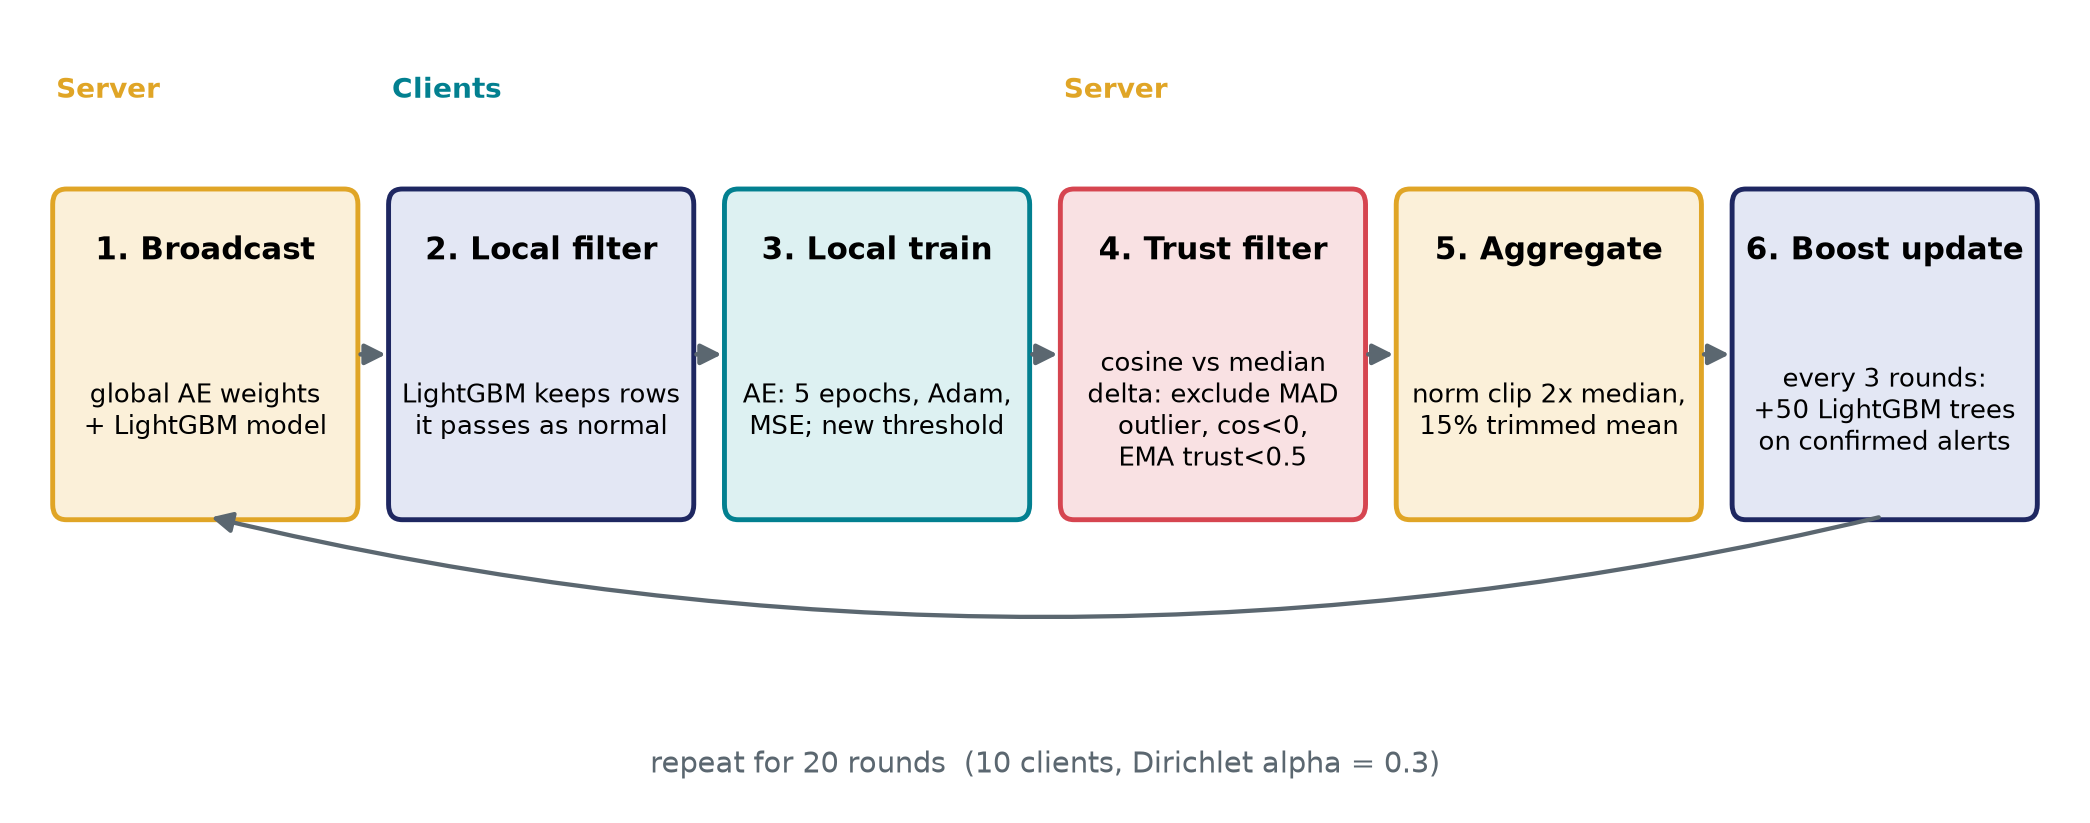
\includegraphics[width=\linewidth]{figures/fl_round.png}
\caption{One federated round}
\label{fig:round}
\end{figure}

\subsection{Incremental classifier update}
Every 3 rounds, each client that survived the filter surfaces up to 50 rows its autoencoder flagged, with analyst-confirmed labels. The server continues training LightGBM with 50 more trees on the calibration set plus all collected alerts, or retrains from scratch if the alerts contain a class the model has never seen. This relaxes the ``no raw traffic leaves a client'' rule for these capped, confirmed alerts only, and is reported as a privacy trade-off.

\subsection{SDN mitigation}
In Phase B, Mininet creates one host per federated client on one Open vSwitch switch, controlled by os-ken over OpenFlow~1.3. A real attack capture is replayed with tcpreplay. TShark extracts all 61 of the dataset's fields, the service-port, content and flow features are derived from the capture with the same code as in training, each row is scored with that host's own scaler and threshold, and the most frequent non-benign label becomes the device verdict. A Flask bridge maps the verdict to an action: \emph{block} (a drop rule on the source IP) if confidence $\geq0.85$, \emph{rate-limit} (an OpenFlow meter) if $\geq0.5$, otherwise allow. The installed rule is then read back from the switch's flow table to confirm it.

\subsection{Evaluation metrics}
With $TP_k$, $FP_k$, $FN_k$ counted per class $k$ over $K$ classes:
\begin{align}
  \text{Accuracy} &= \frac{\#\text{correct}}{\#\text{test rows}}, &
  P_k &= \frac{TP_k}{TP_k+FP_k}, &
  R_k &= \frac{TP_k}{TP_k+FN_k},\\
  F1_k &= \frac{2P_kR_k}{P_k+R_k}, &
  \text{Macro F1} &= \frac{1}{K}\sum_{k}F1_k .
\end{align}
Because 71\% of traffic is benign, accuracy alone hides poor results on rare attacks, so macro F1 is reported next to it. A class with no rows in a test split (MITM is a single flow) is left out of that split's macro average. Two splits are used: a \textbf{stratified random 80/20 split} of rows, and a stricter \textbf{flow-grouped 80/20 split} (stratified group k-fold), in which every flow lies entirely in training or entirely in test, so the model cannot score well by memorising connections. The \textbf{ambiguity ceiling}, the accuracy of an oracle that gives every distinct feature vector its majority label, shows how separable the classes are with a given feature set. For the federated system, attack macro-recall, benign false-positive rate, zero-day macro-recall (leave one attack class out of all training data, then score it) and malicious-client survival rate are also reported.

\chapter{Results and Discussion}\label{chap:results}

\section{Presentation of Results}
All numbers in this chapter come from logged runs on the hardware in Section~\ref{sec:hw}. Unless stated otherwise, the seed is 42. The chapter is ordered from the strongest evidence to the weakest: the stand-alone classifier (Section~\ref{sec:clfacc}), the whole federated system on the whole dataset split by connection (Section~\ref{sec:fullpool}), how long training and a decision take (Section~\ref{sec:speed}), the comparison with a deep-learning classifier, and finally the earlier experiments on a 60{,}000-row pool, which are kept for comparison (Section~\ref{sec:earlier}).

\textbf{Scale of the results.} The earlier experiments use a 60{,}000-row federated pool split row by row, to keep roughly 150 evaluation runs practical. The full-dataset experiments repeat the federated system on all 1{,}985{,}768 usable rows, split by connection, and give the headline federated results.

\subsection{Classifier accuracy}\label{sec:clfacc}
The project requirement was at least 95\% accuracy and at least 0.95 macro F1. The earlier classifier comparison, on a 500{,}000-row class-balanced sample of the base features, gave 0.891 accuracy and 0.887 macro F1. On all 1.9 million rows with the natural class distribution, the same base features give 0.964 accuracy but still only 0.887 macro F1, because the application-layer attacks are confused with each other.

The final classifier is trained on 1{,}429{,}825 packets and tested on 397{,}073 packets from connections it never saw (Table~\ref{tab:datascale}).

\subsubsection{Ambiguity ceiling}
Before tuning the model, we measured how many rows are impossible to separate with each feature set (Table~\ref{tab:ceiling}). With the 91 base features, 2.31\% of rows share an identical feature vector with a row of a different class, which caps macro recall at 0.969 for \emph{any} per-packet classifier. The new features bring the ambiguous share down to 0.01\%.
\begin{table}[H]
\centering
\renewcommand{\arraystretch}{1.2}
\begin{tabular}{|l|c|c|c|c|}
\hline
\textbf{Feature set} & \textbf{Features} & \textbf{Ambiguous} & \textbf{Ceiling acc.} & \textbf{Ceiling macro rec.} \\ \hline
Base & 91 & 2.31\% & 0.9875 & 0.9692 \\ \hline
+ service port & 92 & 0.29\% & 0.9985 & 0.9940 \\ \hline
+ content + flow & 130 & 0.01\% & 0.9999 & 0.9997 \\ \hline
\end{tabular}
\caption{Ambiguity ceiling per feature set (all rows, after de-duplication)}
\label{tab:ceiling}
\end{table}

\subsubsection{Effect of each feature group}
Table~\ref{tab:progression} and Figure~\ref{fig:progression} add the feature groups one at a time, on the strict flow-grouped split. The service port mainly fixes Normal versus attack traffic. The content features add little on their own, because only a small share of packets carries content. The flow features give the largest jump, because they pass a connection's content and behaviour on to its content-free packets. Class weighting then stabilises the rare Fingerprinting class.
\begin{table}[H]
\centering
\renewcommand{\arraystretch}{1.2}
\begin{tabular}{|l|c|c|c|c|}
\hline
 & \multicolumn{2}{c|}{\textbf{Random split}} & \multicolumn{2}{c|}{\textbf{Flow-grouped split}} \\ \hline
\textbf{Features} & \textbf{Accuracy} & \textbf{Macro F1} & \textbf{Accuracy} & \textbf{Macro F1} \\ \hline
Base (91) & 0.9638 & 0.8868 & 0.9637 & 0.8892 \\ \hline
+ service port (92) & 0.9802 & 0.9245 & 0.9803 & 0.9236 \\ \hline
+ content (110) & 0.9802 & 0.9268 & 0.9802 & 0.9232 \\ \hline
+ flow (130) & 0.9977 & 0.9879 & 0.9975 & 0.9808 \\ \hline
\textbf{+ class weights (final)} & \textbf{0.9976} & \textbf{0.9867} & \textbf{0.9972} & \textbf{0.9828} \\ \hline
\end{tabular}
\caption{Accuracy and macro F1 as feature groups are added (LightGBM, all rows, 80/20)}
\label{tab:progression}
\end{table}
\begin{figure}[H]
\centering
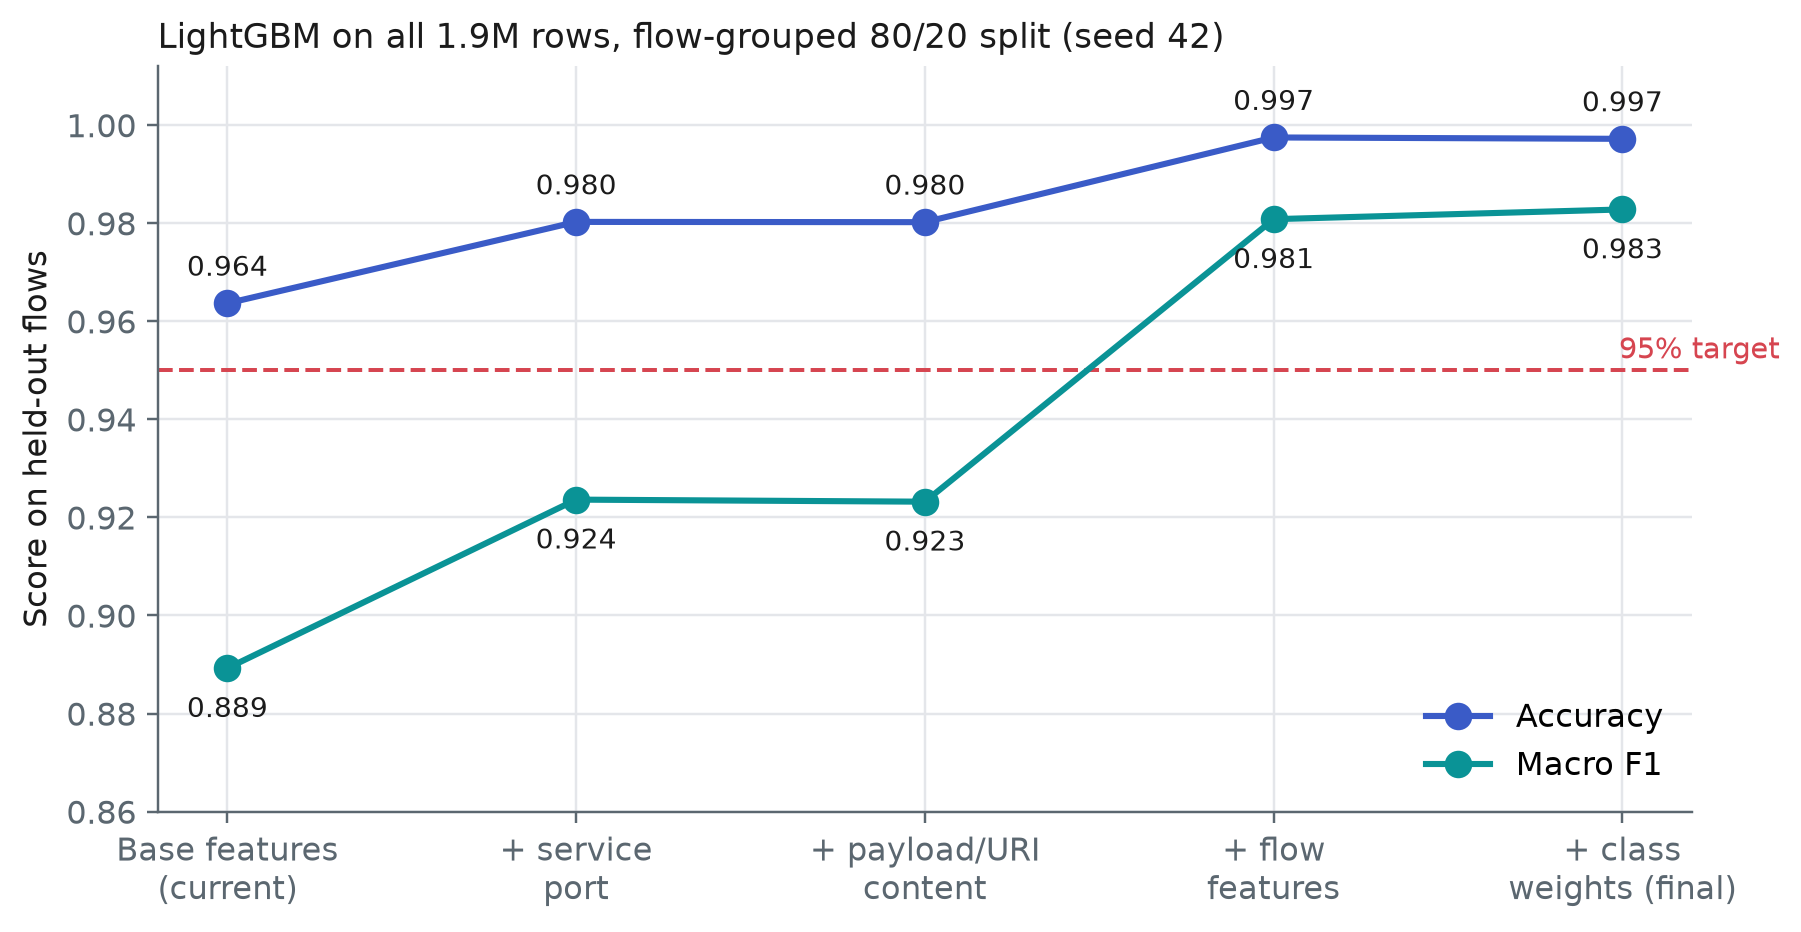
\includegraphics[width=0.92\linewidth]{figures/accuracy_progression.png}
\caption{Accuracy and macro F1 on held-out flows as each feature group is added}
\label{fig:progression}
\end{figure}

\subsubsection{Robustness across seeds, splits and training size}
Table~\ref{tab:seeds} repeats the final configuration with three seeds on both splits. Accuracy stays between 0.9970 and 0.9977, and macro F1 between 0.9828 and 0.9868. Without class weights, the flow-grouped macro F1 was less stable (0.9808, 0.9560, 0.9521), because the Fingerprinting score depended on which of its 156 flows landed in test. Weighting removes that sensitivity.

\begin{table}[H]
\centering
\renewcommand{\arraystretch}{1.2}
\begin{tabular}{|l|c|c|c|}
\hline
\textbf{Split / seed} & \textbf{42} & \textbf{43} & \textbf{44} \\ \hline
Random: accuracy & 0.9976 & 0.9977 & 0.9976 \\ \hline
Random: macro F1 & 0.9867 & 0.9868 & 0.9866 \\ \hline
Flow-grouped: accuracy & 0.9972 & 0.9971 & 0.9970 \\ \hline
Flow-grouped: macro F1 & 0.9828 & 0.9835 & 0.9851 \\ \hline
\end{tabular}
\caption{Final classifier across seeds}
\label{tab:seeds}
\end{table}

Two further checks were run. \textbf{(a) Same sampling as before:} on a 500{,}000-row capped sample drawn the same way as in the earlier boosting-versus-DL comparison, and with the same training settings for both feature sets, accuracy rises from 0.8902 to 0.9919 and macro F1 from 0.8827 to 0.9900. \textbf{(b) Calibration-set size:} in FL-IDS the server trains LightGBM on only a 5\% calibration set. Trained on 5\% of the rows and tested on held-out flows, the new features give 0.9968 accuracy and 0.9791 macro F1, against 0.9624 and 0.8807 for the base features. The gain therefore carries over to the classifier as the federated system actually trains it.

\subsubsection{Per-class results}
Figure~\ref{fig:perclass} compares per-class F1 before and after. The biggest gains are on exactly the classes that were weak: Uploading (0.76 to 1.00), DDoS\_HTTP (0.76 to 0.97), SQL\_injection (0.80 to 1.00), Password (0.84 to 0.97), XSS (0.85 to 0.98) and Fingerprinting (0.68 to 0.93). Figure~\ref{fig:cm} shows the remaining confusion: Password and DDoS\_HTTP traffic (both HTTP requests to the same server) and Ransomware versus Backdoor (both on port 4321). MITM is a single ARP flow, so it cannot be scored on the flow-grouped split; on the random split its F1 is 0.994.
\begin{figure}[H]
\centering
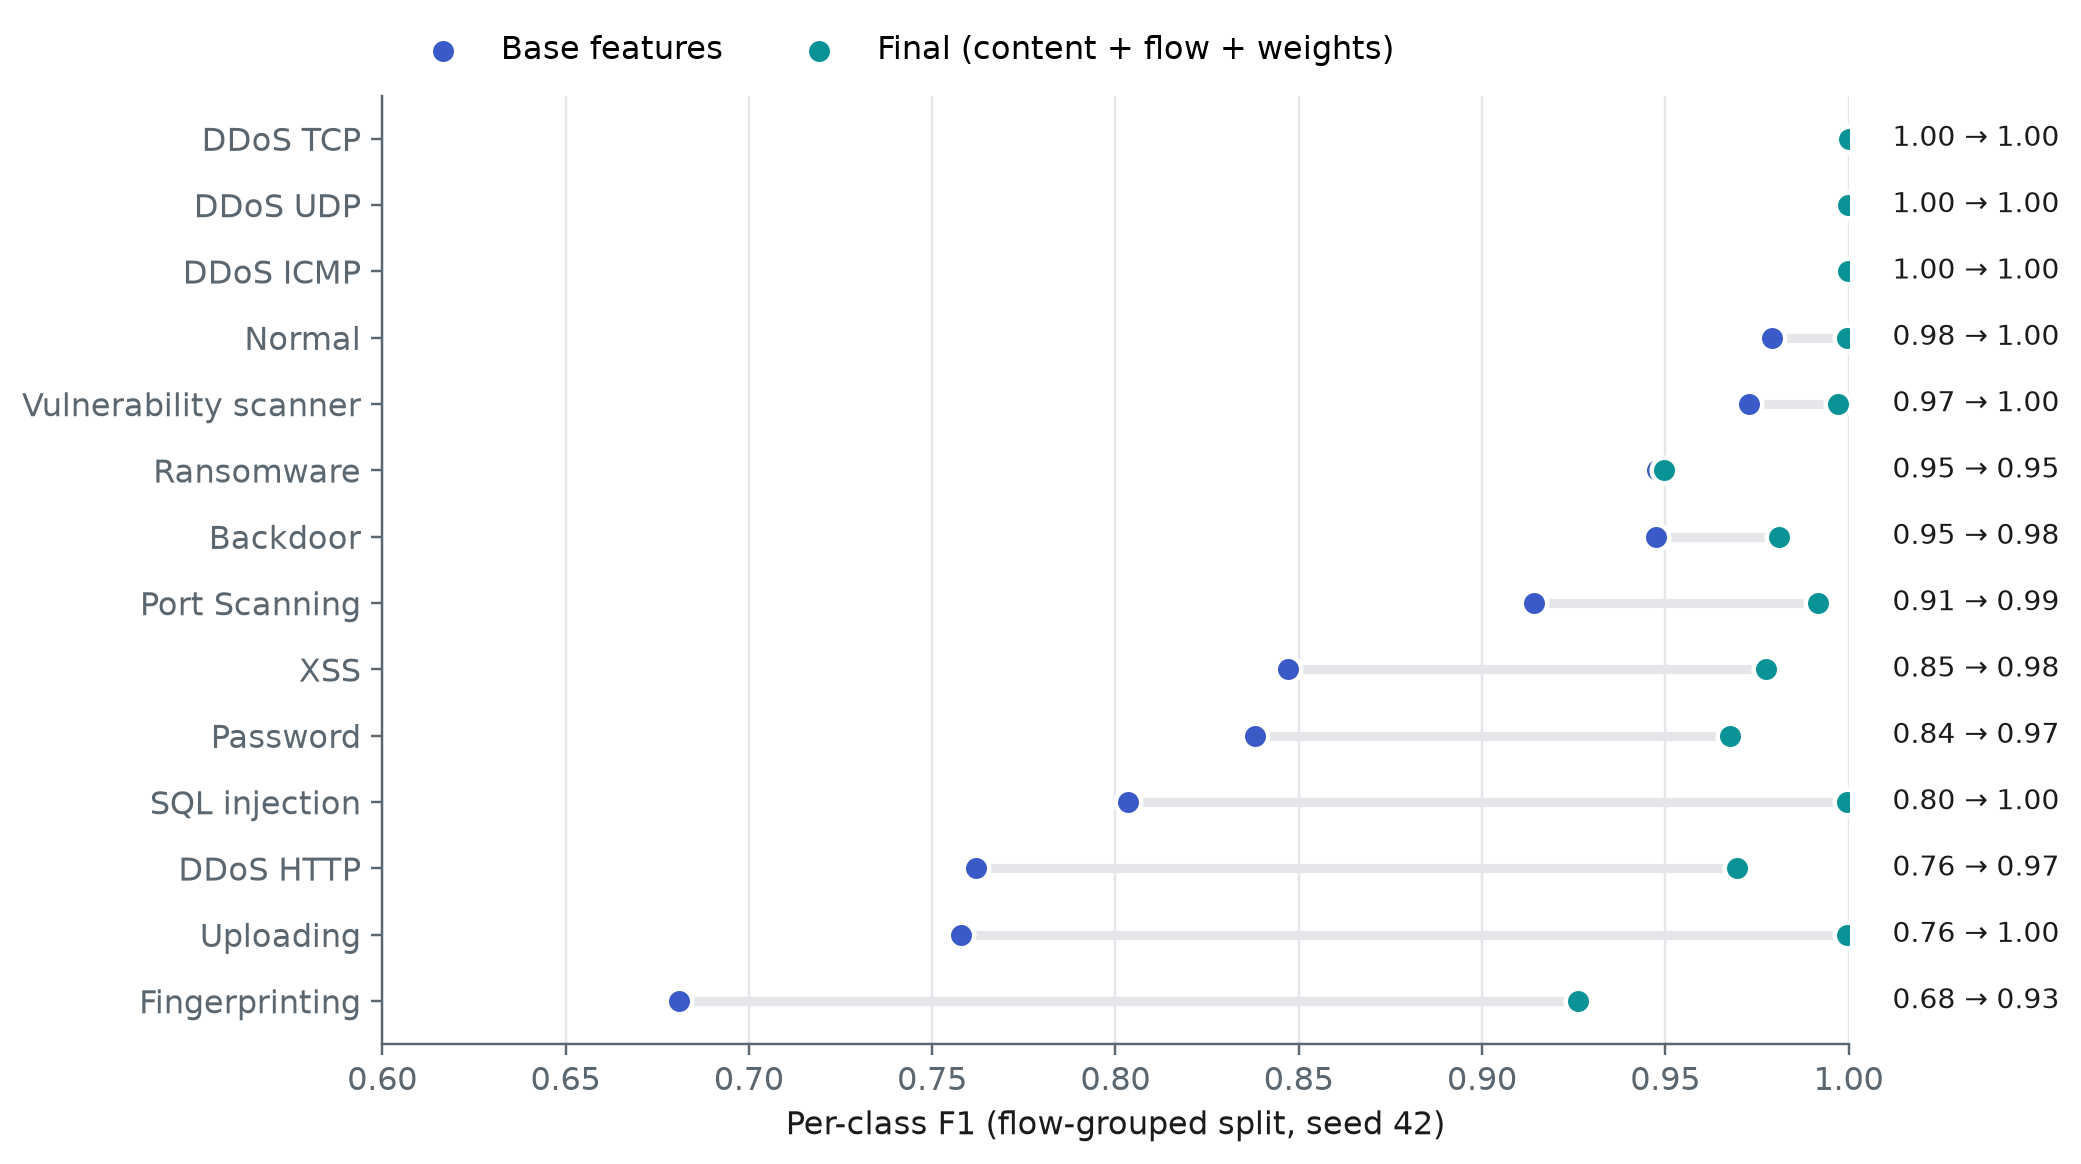
\includegraphics[width=0.88\linewidth]{figures/per_class_f1.png}
\caption{Per-class F1, base features vs.\ final classifier (flow-grouped split)}
\label{fig:perclass}
\end{figure}
\begin{figure}[H]
\centering
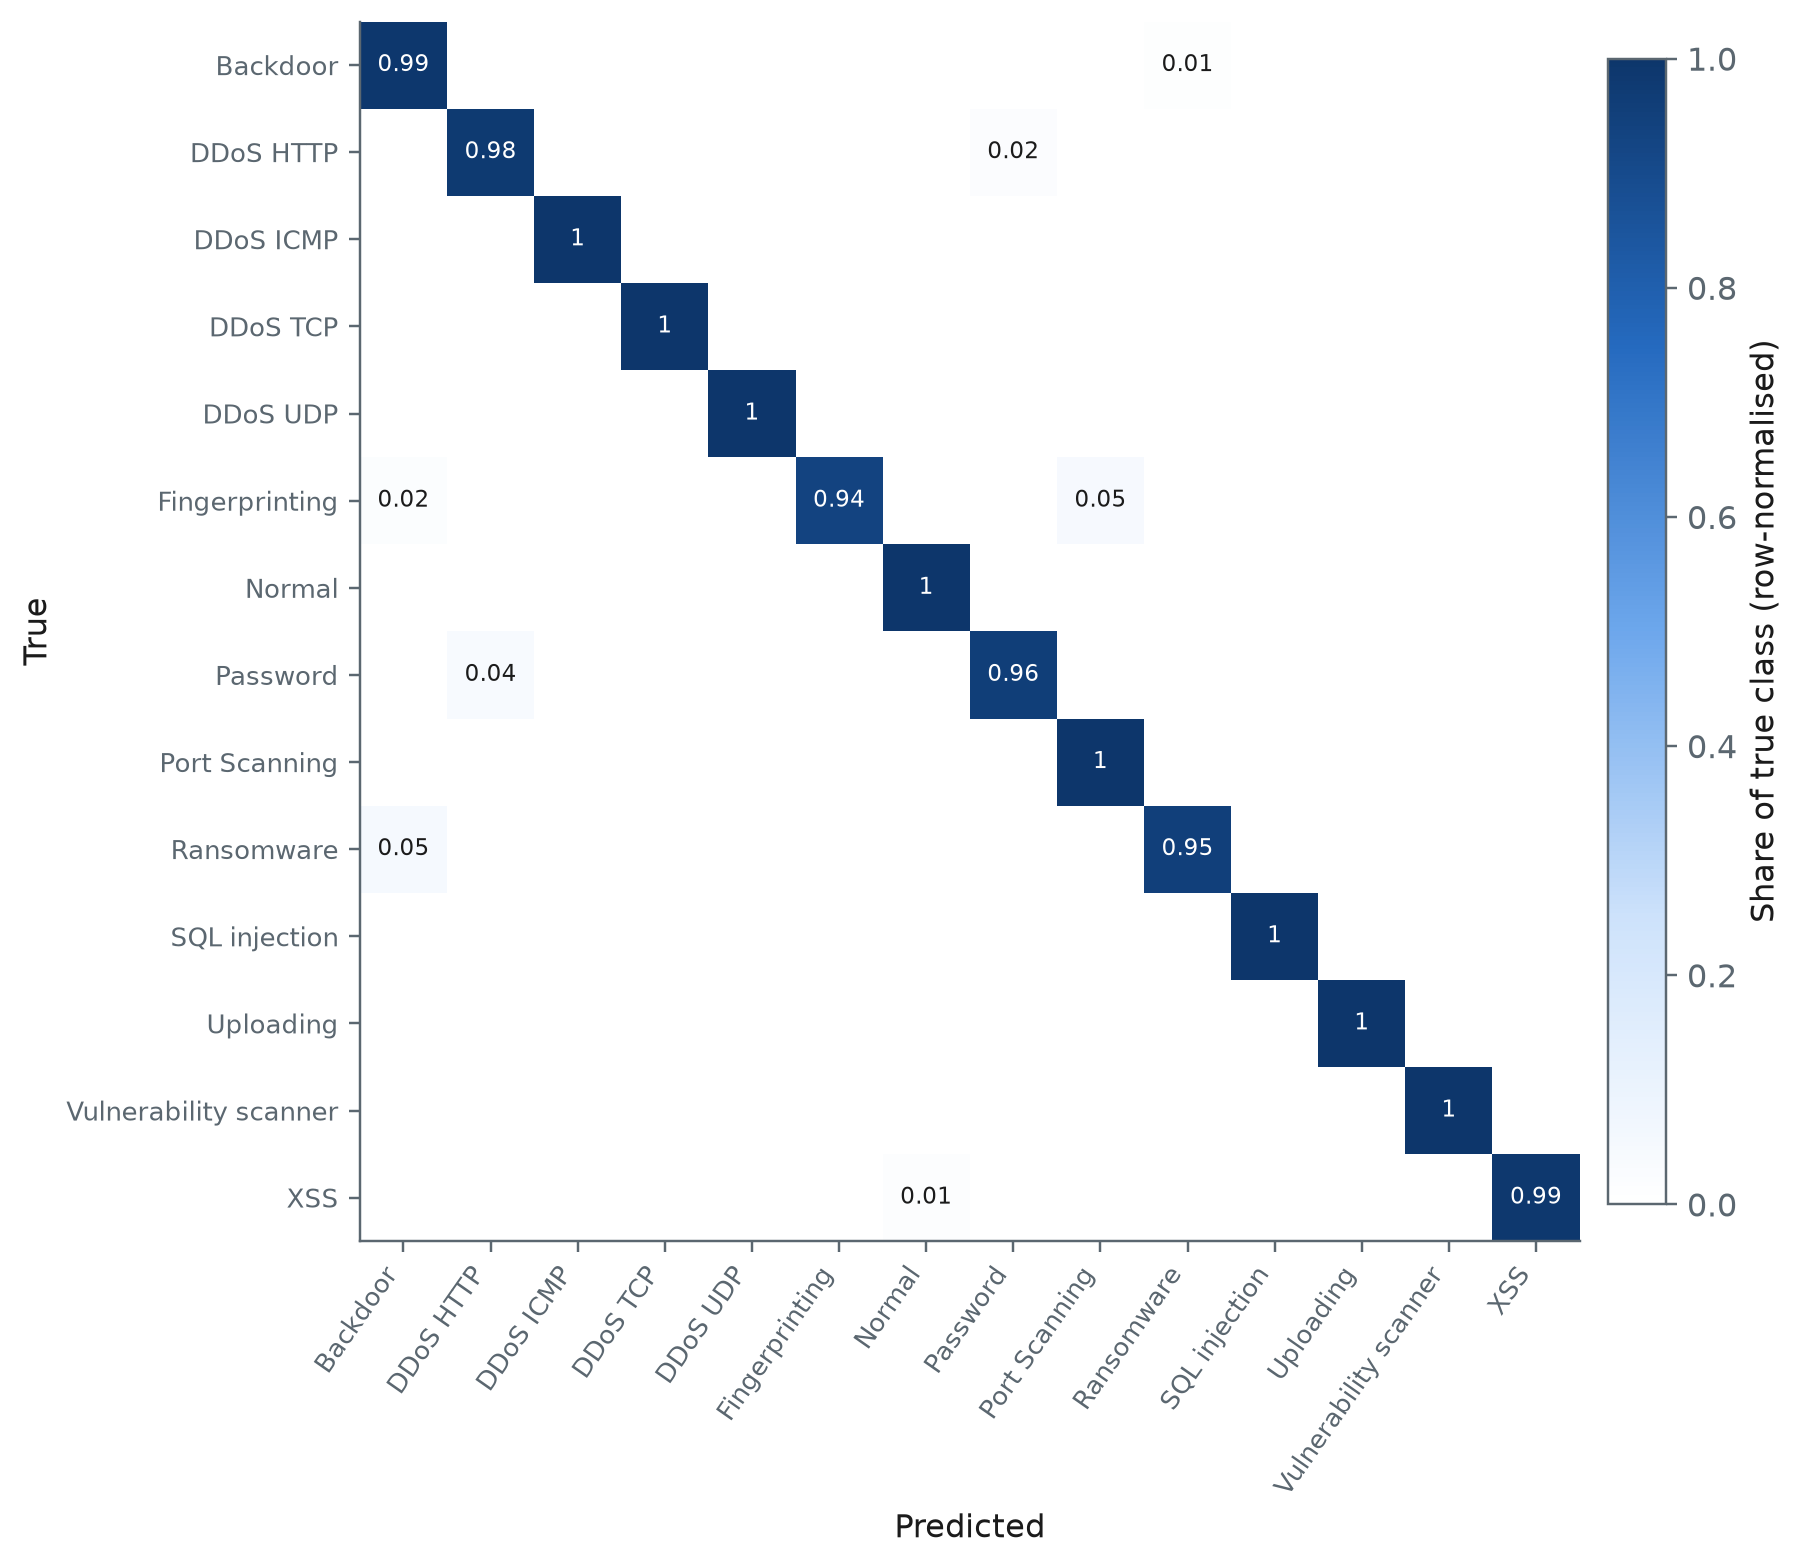
\includegraphics[width=0.8\linewidth]{figures/confusion_final.png}
\caption{Row-normalised confusion matrix of the final classifier (flow-grouped split)}
\label{fig:cm}
\end{figure}

\subsubsection{Discussion and caveats}
\begin{itemize}
  \item \textbf{Why a flow-grouped split matters.} A random split of packets puts packets of the same connection in both training and test sets. Reporting the stricter split shows that the improvement does not come from memorising connections.
  \item \textbf{The service port is partly a testbed effect.} In Edge-IIoTset, benign traffic is MQTT (port 1883) and VNC (5900) and never HTTP. In a real network with benign web traffic, the port alone would separate much less.
  \item \textbf{Flow features are computed over the whole flow record} (up to 120\,s), the same way as CICFlowMeter. The classifier therefore labels flow records rather than making a decision on the first packet.
  \item The same features are used by the whole federated pipeline and by Phase B. The following sections report the system-level results with them, next to the original 91-feature results.
\end{itemize}

\subsection{The whole system on the full dataset, split by connection}\label{sec:fullpool}
All of the federated results in the earlier sections of this chapter use a 60{,}000-row pool split row by row. This section repeats the federated experiments on all 1{,}985{,}768 usable rows. The server keeps a labelled calibration set (71{,}853 to 79{,}866 rows, about 5\%, depending on the seed) to bootstrap the classifier; the other 1{,}885{,}587 to 1{,}885{,}744 rows are split across 10 or 20 clients, whose test slices hold 283{,}090 to 295{,}566 rows (about 9{,}000 before). Packets of one connection share their flow-level features, so a row-level split puts near-identical siblings on both sides of a test. Here every connection stays whole: in the calibration set, in exactly one client, and in exactly one of that client's training, benign-validation and test slices. MITM is a single connection, so it cannot be split; all of it goes to the server's calibration set (the classifier learns it) and it is scored by the zero-day experiment and the live replay only.

\textbf{A leak check first.} At the old 60{,}000-row scale, splitting by connection did not lower known-attack recall (the classifier alone caught 0.9962 of attack packets, against 0.9968 with the row split), so the earlier federated recall numbers were not inflated by sibling packets.

\textbf{Real runs.} Table~\ref{tab:full_real_full} lists six real multi-process runs (one server and 10 or 20 client processes, 20 rounds, three seeds). Known attacks are caught as before: micro recall 0.9956 to 0.9989 and classifier-alone micro recall 0.9954 to 0.9981 (0.9939 to 0.9980 in the earlier runs; Table~\ref{tab:full_pool_compare}). False alarms need two numbers. Counted per packet, 2.5\% to 16.3\% of normal test packets are flagged (earlier 2.8\% to 4.0\%), but counted per connection the rate is 0.34\% to 1.04\%, and the median client flags 2.9\% to 3.2\% of its packets in all six runs. The packet figure is dominated by a few very long normal connections (7{,}000 to 11{,}800 packets each): in five of the six runs, 80\% to 94\% of the false-alarm packets come from the ten largest connections. The false-alarm rate should therefore be quoted both ways.

\begin{table}[H]
\centering
\scriptsize
\setlength{\tabcolsep}{3pt}
\renewcommand{\arraystretch}{1.15}
\begin{tabular}{|l|c|c|c|c|c|c|c|c|}
\hline
\textbf{Run} & \textbf{Phase A s} & \textbf{Attack macro-recall} & \textbf{Attack micro recall} & \textbf{Classifier-only micro recall} & \textbf{Packet-level false alarms} & \textbf{Connection-level false alarms} & \textbf{Test rows} & \textbf{Clients with no benign validation rows} \\ \hline
10 clients, seed 42 & 1844 & 0.9958 & 0.9974 & 0.9970 & 0.1275 & 0.0034 & 288,416 & 1 \\ \hline
10 clients, seed 43 & 1397 & 0.9947 & 0.9978 & 0.9971 & 0.0884 & 0.0074 & 283,090 & 0 \\ \hline
10 clients, seed 44 & 1754 & 0.9939 & 0.9956 & 0.9954 & 0.0248 & 0.0039 & 288,366 & 2 \\ \hline
20 clients, seed 42 & 1260 & 0.9981 & 0.9989 & 0.9981 & 0.0588 & 0.0104 & 283,427 & 3 \\ \hline
20 clients, seed 43 & 1063 & 0.9970 & 0.9980 & 0.9974 & 0.1628 & 0.0076 & 292,222 & 2 \\ \hline
20 clients, seed 44 & 1225 & 0.9972 & 0.9978 & 0.9972 & 0.1089 & 0.0081 & 295,566 & 0 \\ \hline
\end{tabular}
\caption{Real multi-process Phase A on the full pool (1.89M rows), split by connection, 20 rounds, no attackers}
\label{tab:full_real_full}
\end{table}
\begin{table}[H]
\centering
\scriptsize
\setlength{\tabcolsep}{3pt}
\renewcommand{\arraystretch}{1.15}
\begin{tabular}{|l|c|c|c|c|}
\hline
\textbf{Setting} & \textbf{Attack macro-recall} & \textbf{Attack micro recall} & \textbf{Classifier-only micro recall} & \textbf{Benign FPR (packets)} \\ \hline
10 clients, seed 42: 60k pool, split by row & 0.9990 & 0.9992 & 0.9968 & 0.0340 \\ \hline
10 clients, seed 42: full pool, split by connection & 0.9958 & 0.9974 & 0.9970 & 0.1275 \\ \hline
10 clients, seed 42: 60k pool, split by connection & 1.0000 & 1.0000 & 0.9962 & 0.0443 \\ \hline
10 clients, seed 43: 60k pool, split by row & 0.9985 & 0.9992 & 0.9976 & 0.0311 \\ \hline
10 clients, seed 43: full pool, split by connection & 0.9947 & 0.9978 & 0.9971 & 0.0884 \\ \hline
10 clients, seed 44: 60k pool, split by row & 0.9962 & 0.9960 & 0.9939 & 0.0284 \\ \hline
10 clients, seed 44: full pool, split by connection & 0.9939 & 0.9956 & 0.9954 & 0.0248 \\ \hline
20 clients, seed 42: 60k pool, split by row & 0.9784 & 0.9964 & 0.9952 & 0.0362 \\ \hline
20 clients, seed 42: full pool, split by connection & 0.9981 & 0.9989 & 0.9981 & 0.0588 \\ \hline
20 clients, seed 43: 60k pool, split by row & 0.9993 & 0.9992 & 0.9980 & 0.0284 \\ \hline
20 clients, seed 43: full pool, split by connection & 0.9970 & 0.9980 & 0.9974 & 0.1628 \\ \hline
20 clients, seed 44: 60k pool, split by row & 0.9991 & 0.9988 & 0.9968 & 0.0396 \\ \hline
20 clients, seed 44: full pool, split by connection & 0.9972 & 0.9978 & 0.9972 & 0.1089 \\ \hline
\end{tabular}
\caption{The same runs at the earlier scale and now (macro-recall includes only attack types present in the test slices)}
\label{tab:full_pool_compare}
\end{table}
\begin{figure}[H]
\centering
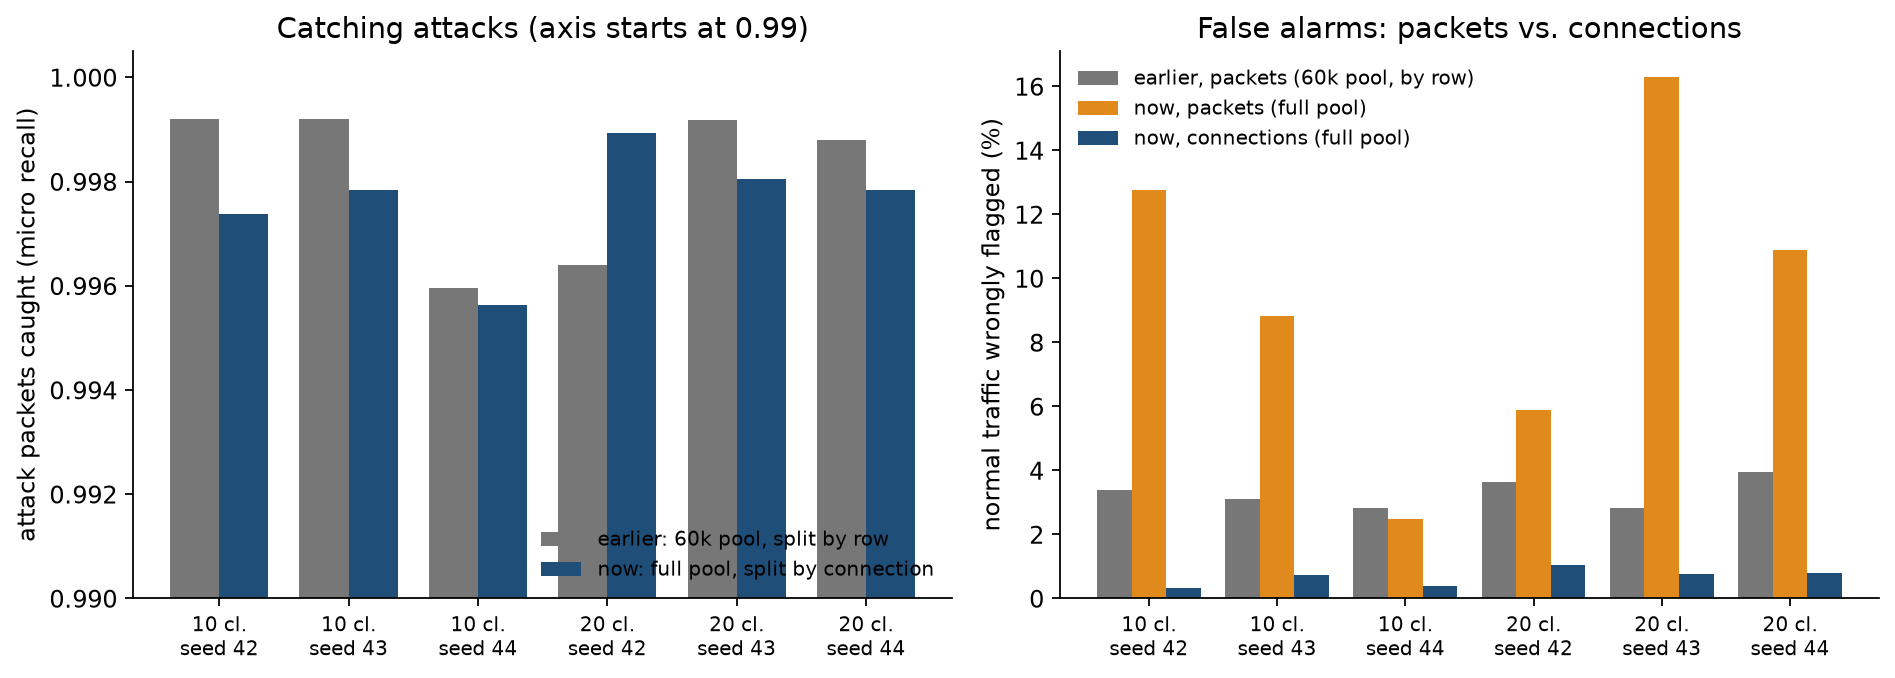
\includegraphics[width=0.95\linewidth]{figures/full_pool_runs.png}
\caption{Earlier (60k pool, split by row) and full-pool (split by connection) results for the six runs}
\label{fig:fullpoolruns}
\end{figure}
\begin{table}[H]
\centering
\scriptsize
\setlength{\tabcolsep}{3pt}
\renewcommand{\arraystretch}{1.15}
\begin{tabular}{|l|c|c|c|c|}
\hline
\textbf{Class} & \textbf{Test rows} & \textbf{Classifier alone} & \textbf{Autoencoder alone} & \textbf{Cascade} \\ \hline
Backdoor & 2263 & 0.9885 & 0.0367 & 0.9929 \\ \hline
DDoS\_HTTP & 6915 & 0.9899 & 0.4807 & 0.9899 \\ \hline
DDoS\_ICMP & 9520 & 1.0000 & 0.3171 & 1.0000 \\ \hline
DDoS\_TCP & 6717 & 1.0000 & 0.9394 & 1.0000 \\ \hline
DDoS\_UDP & 17755 & 0.9999 & 0.3063 & 1.0000 \\ \hline
Fingerprinting & 129 & 0.9845 & 0.0698 & 0.9922 \\ \hline
Password & 7795 & 0.9913 & 0.2517 & 0.9914 \\ \hline
Port\_Scanning & 2929 & 1.0000 & 0.6842 & 1.0000 \\ \hline
Ransomware & 691 & 0.9841 & 0.4877 & 0.9870 \\ \hline
SQL\_injection & 7228 & 0.9990 & 0.8944 & 0.9996 \\ \hline
Uploading & 5567 & 0.9998 & 0.5493 & 0.9998 \\ \hline
Vulnerability\_scanner & 7216 & 0.9946 & 0.5006 & 0.9961 \\ \hline
XSS & 2274 & 0.9960 & 0.4714 & 0.9969 \\ \hline
\end{tabular}
\caption{Recall per attack type, 10 clients, seed 42, full pool, by stage (held-out test slices)}
\label{tab:full_per_class}
\end{table}
\textbf{Poisoning and ablation.} Known-attack recall stays between 0.985 and 0.997 at every attacker fraction up to 50\% (Table~\ref{tab:full_sweep}). The trust filter lets more attackers through than at 60{,}000 rows: attacker survival at 30\% is 0.50, 0.55 and 0.62 (earlier 0.12, 0.12 and 0.27), and at 50\% it is 0.64, 1.00 and 0.99; why is not established. Robust aggregation still protects the autoencoder: with 30\% attackers its recall alone is 0.490, 0.373 and 0.245 for the full pipeline, against 0.013, 0.002 and 0.092 for plain FedAvg (Table~\ref{tab:full_ablation}). The ranges are wide and three seeds support no confidence intervals. The ablation's full-pipeline row is the sweep's 30\% point.

\begin{table}[H]
\centering
\small
\setlength{\tabcolsep}{3pt}
\renewcommand{\arraystretch}{1.15}
\begin{tabular}{|l|c|c|c|}
\hline
\textbf{Attackers} & \textbf{Attack macro-recall} & \textbf{Autoencoder-alone recall} & \textbf{Attacker survival} \\ \hline
0\% & 0.996 / 0.996 / 0.994 & 0.457 / 0.492 / 0.221 & n/a / n/a / n/a \\ \hline
20\% & 0.995 / 0.996 / 0.994 & 0.466 / 0.483 / 0.258 & 0.30 / 0.40 / 0.23 \\ \hline
30\% & 0.995 / 0.997 / 0.995 & 0.490 / 0.373 / 0.245 & 0.50 / 0.55 / 0.62 \\ \hline
40\% & 0.994 / 0.994 / 0.992 & 0.297 / 0.139 / 0.074 & 0.60 / 0.64 / 0.61 \\ \hline
50\% & 0.995 / 0.990 / 0.985 & 0.249 / 0.000 / 0.000 & 0.64 / 1.00 / 0.99 \\ \hline
\end{tabular}
\caption{Poisoning sweep, full pool}
\label{tab:full_sweep}
\end{table}
\begin{table}[H]
\centering
\small
\setlength{\tabcolsep}{3pt}
\renewcommand{\arraystretch}{1.15}
\begin{tabular}{|l|c|c|c|}
\hline
\textbf{Variant} & \textbf{Attack macro-recall} & \textbf{Autoencoder-alone recall} & \textbf{Benign FPR} \\ \hline
full\_pipeline & 0.995 / 0.997 / 0.995 & 0.490 / 0.373 / 0.245 & 0.1112 / 0.0653 / 0.0075 \\ \hline
autoencoder\_only & 0.105 / 0.073 / 0.051 & 0.105 / 0.073 / 0.051 & 0.0473 / 0.0411 / 0.0445 \\ \hline
boosting\_only & 0.990 / 0.989 / 0.982 & n/a / n/a / n/a & 0.0001 / 0.0001 / 0.0003 \\ \hline
plain\_fedavg & 0.992 / 0.994 / 0.990 & 0.013 / 0.002 / 0.092 & 0.0947 / 0.0301 / 0.0301 \\ \hline
trimmed\_mean\_only & 0.995 / 0.995 / 0.993 & 0.205 / 0.000 / 0.025 & 0.1070 / 0.0261 / 0.0299 \\ \hline
\end{tabular}
\caption{Ablation at 30\% sign-flip attackers, full pool, seeds 42 / 43 / 44}
\label{tab:full_ablation}
\end{table}
\textbf{Zero-day detection.} The cascade detects 0.910, 0.944 and 0.895 of an unseen attack type on average (earlier 0.943, 0.952 and 0.952); every row of each held-out class is scored (Tables~\ref{tab:full_zeroday_mean} and~\ref{tab:full_zeroday_class}, Figure~\ref{fig:fullzd}). Uploading is the weakest (0.527 to 0.665), followed by MITM (0.751 to 1.000) and, depending on the seed, Backdoor and Vulnerability\_scanner.

\begin{table}[H]
\centering
\small
\setlength{\tabcolsep}{3pt}
\renewcommand{\arraystretch}{1.15}
\begin{tabular}{|l|c|}
\hline
\textbf{Stage} & \textbf{Mean detection rate} \\ \hline
Classifier alone & 0.735 / 0.757 / 0.723 (classes: 14, 14, 14) \\ \hline
Autoencoder alone & 0.681 / 0.728 / 0.590 (classes: 14, 14, 14) \\ \hline
Cascade & 0.910 / 0.944 / 0.895 (classes: 14, 14, 14) \\ \hline
\end{tabular}
\caption{Zero-day (leave one attack class out), full pool: mean over the held-out classes}
\label{tab:full_zeroday_mean}
\end{table}
\begin{table}[H]
\centering
\scriptsize
\setlength{\tabcolsep}{3pt}
\renewcommand{\arraystretch}{1.15}
\begin{tabular}{|l|c|c|c|c|}
\hline
\textbf{Held-out class} & \textbf{Rows scored} & \textbf{Cascade detection} & \textbf{Classifier alone} & \textbf{Autoencoder alone} \\ \hline
Backdoor & 24167 & 0.743 / 0.998 / 0.998 & 0.486 / 0.996 / 0.997 & 0.493 / 0.550 / 0.810 \\ \hline
DDoS\_HTTP & 49768 & 0.879 / 0.932 / 0.885 & 0.695 / 0.764 / 0.719 & 0.572 / 0.698 / 0.560 \\ \hline
DDoS\_ICMP & 68758 & 1.000 / 1.000 / 1.000 & 1.000 / 1.000 / 0.999 & 0.786 / 0.802 / 0.800 \\ \hline
DDoS\_TCP & 50062 & 0.933 / 0.953 / 0.921 & 0.865 / 0.921 / 0.879 & 0.640 / 0.686 / 0.615 \\ \hline
DDoS\_UDP & 121567 & 0.905 / 0.803 / 0.866 & 0.416 / 0.021 / 0.334 & 0.849 / 0.799 / 0.799 \\ \hline
Fingerprinting & 872 & 0.998 / 0.998 / 0.997 & 0.995 / 0.994 / 0.994 & 0.826 / 0.747 / 0.492 \\ \hline
MITM & 406 & 0.803 / 1.000 / 0.751 & 0.148 / 0.200 / 0.005 & 0.764 / 1.000 / 0.751 \\ \hline
Password & 50033 & 0.932 / 0.935 / 0.880 & 0.872 / 0.865 / 0.813 & 0.505 / 0.407 / 0.307 \\ \hline
Port\_Scanning & 20213 & 0.999 / 0.993 / 0.992 & 0.998 / 0.988 / 0.989 & 0.570 / 0.745 / 0.409 \\ \hline
Ransomware & 9885 & 0.990 / 0.994 / 0.988 & 0.984 / 0.990 / 0.982 & 0.621 / 0.753 / 0.374 \\ \hline
SQL\_injection & 50981 & 0.961 / 0.970 / 0.999 & 0.828 / 0.713 / 0.999 & 0.764 / 0.871 / 0.787 \\ \hline
Uploading & 37243 & 0.665 / 0.652 / 0.527 & 0.204 / 0.266 / 0.304 & 0.581 / 0.512 / 0.295 \\ \hline
Vulnerability\_scanner & 50044 & 0.992 / 0.993 / 0.859 & 0.980 / 0.894 / 0.335 & 0.880 / 0.976 / 0.772 \\ \hline
XSS & 15172 & 0.943 / 0.991 / 0.867 & 0.823 / 0.986 / 0.767 & 0.680 / 0.650 / 0.483 \\ \hline
\end{tabular}
\caption{Zero-day (leave one attack class out), full pool: mean over the held-out classes: per held-out class}
\label{tab:full_zeroday_class}
\end{table}
\begin{figure}[H]
\centering
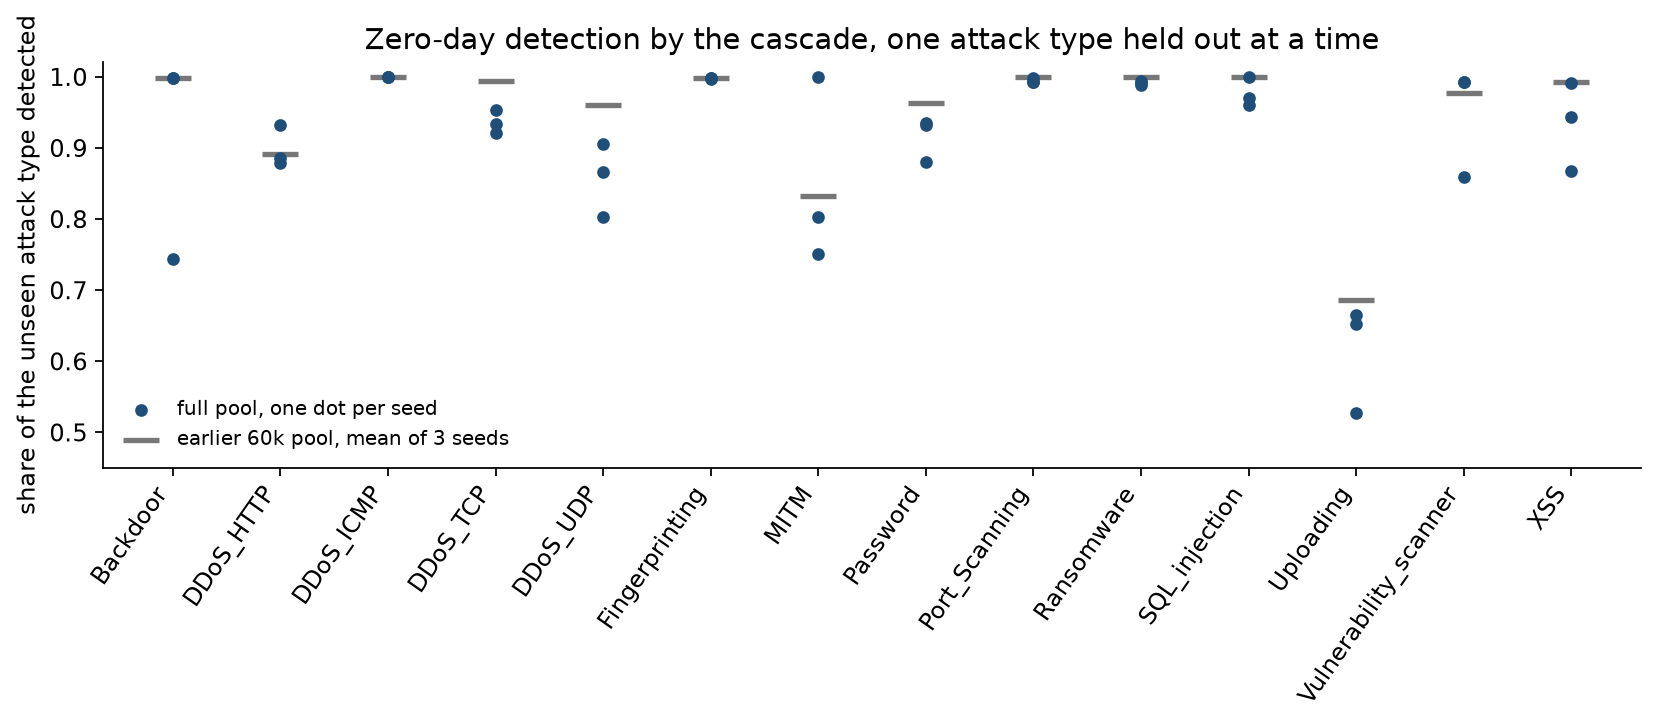
\includegraphics[width=0.9\linewidth]{figures/full_zero_day.png}
\caption{Zero-day detection by the cascade at full scale (one dot per seed) and the earlier 60k-pool mean}
\label{fig:fullzd}
\end{figure}
\textbf{Stealth attacker, pruning and clipping (seed 42 only).} The stealth attacker survives in 0.60, 0.73 and 0.80 of client-rounds against 0.30, 0.50 and 0.60 for sign-flip, with no clear extra harm to the autoencoder and known-attack recall of at least 0.9949 (Table~\ref{tab:full_stealth}). Pruning during training costs more at full scale than at 60{,}000 rows: autoencoder-alone recall falls from 0.457 to 0.350 at 70\% sparsity, and to 0.098 when pruned after training (Table~\ref{tab:full_pruning}). Without the per-client clip the final benign validation loss is 0.242 against 0.129 with it, much less than the factor of about 1{,}500 at the smaller scale (Table~\ref{tab:full_clip}).

\begin{table}[H]
\centering
\scriptsize
\setlength{\tabcolsep}{3pt}
\renewcommand{\arraystretch}{1.15}
\begin{tabular}{|l|c|c|c|c|c|}
\hline
\textbf{Attackers} & \textbf{Sign-flip survival} & \textbf{Stealth survival} & \textbf{Sign-flip AE-alone recall} & \textbf{Stealth AE-alone recall} & \textbf{Stealth known-attack recall} \\ \hline
20\% & 0.30 / 0.40 / 0.23 & 0.60 / n/a / n/a & 0.466 / 0.483 / 0.258 & 0.454 / n/a / n/a & 0.9956 / n/a / n/a \\ \hline
30\% & 0.50 / 0.55 / 0.62 & 0.73 / n/a / n/a & 0.490 / 0.373 / 0.245 & 0.427 / n/a / n/a & 0.9961 / n/a / n/a \\ \hline
40\% & 0.60 / 0.64 / 0.61 & 0.80 / n/a / n/a & 0.297 / 0.139 / 0.074 & 0.334 / n/a / n/a & 0.9949 / n/a / n/a \\ \hline
\end{tabular}
\caption{Stealth attacker vs. sign-flip, full pool}
\label{tab:full_stealth}
\end{table}
\begin{table}[H]
\centering
\scriptsize
\setlength{\tabcolsep}{3pt}
\renewcommand{\arraystretch}{1.15}
\begin{tabular}{|l|c|c|c|c|}
\hline
\textbf{Sparsity} & \textbf{Non-zero weights} & \textbf{Autoencoder-alone recall} & \textbf{Cascade macro-recall} & \textbf{Benign FPR} \\ \hline
0\% & 9600 & 0.457 / 0.492 / 0.221 & 0.996 / 0.996 / 0.994 & 0.1182 / 0.0414 / 0.0352 \\ \hline
50\% & 4800 & 0.439 / n/a / n/a & 0.995 / n/a / n/a & 0.1400 / n/a / n/a \\ \hline
70\% & 2880 & 0.350 / n/a / n/a & 0.993 / n/a / n/a & 0.1201 / n/a / n/a \\ \hline
80\% & 1920 & 0.338 / n/a / n/a & 0.993 / n/a / n/a & 0.1451 / n/a / n/a \\ \hline
90\% & 960 & 0.198 / n/a / n/a & 0.993 / n/a / n/a & 0.1151 / n/a / n/a \\ \hline
\end{tabular}
\caption{Pruning during federated training, full pool (no attackers)}
\label{tab:full_pruning}
\end{table}
\begin{table}[H]
\centering
\small
\setlength{\tabcolsep}{3pt}
\renewcommand{\arraystretch}{1.15}
\begin{tabular}{|l|c|c|c|}
\hline
\textbf{Normalisation} & \textbf{seed 42} & \textbf{seed 43} & \textbf{seed 44} \\ \hline
clip 10 & 0.1292 & 0.05736 & 0.2644 \\ \hline
no clip & 0.242 & n/a & n/a \\ \hline
\end{tabular}
\caption{Per-client z-score clip, final-round benign validation loss}
\label{tab:full_clip}
\end{table}
\textbf{Live replay of every capture.} All 14 attack captures were replayed through Mininet with the full-pool bundle (Table~\ref{tab:full_phase_b_all}). Every one ends in a block decision with the drop rule read back from the switch; 12 of 14 are classified as the right attack type, while the MITM capture is called Ransomware and the OS-fingerprinting capture DDoS\_ICMP. The replays are of the dataset's own captures, so they demonstrate the pipeline and are not a held-out test. The released Vulnerability-scanner capture is damaged part-way, so its readable first 265{,}827 packets were used.

\begin{table}[H]
\centering
\scriptsize
\setlength{\tabcolsep}{3pt}
\renewcommand{\arraystretch}{1.15}
\begin{tabular}{|l|c|c|c|c|c|c|}
\hline
\textbf{Capture} & \textbf{Classified as} & \textbf{Confidence} & \textbf{Stage} & \textbf{Packets flagged} & \textbf{Action} & \textbf{Wall time} \\ \hline
Backdoor attack & Backdoor & 0.997 & boosting & 24,543 / 24,914 & block & 12 s \\ \hline
DDoS HTTP Flood Attacks & DDoS\_HTTP & 0.966 & boosting & 119,748 / 229,142 & block & 29 s \\ \hline
DDoS ICMP Flood Attacks & DDoS\_ICMP & 1.000 & boosting & 2,914,156 / 2,914,356 & block & 232 s \\ \hline
DDoS TCP SYN Flood Attacks & DDoS\_TCP & 0.999 & boosting & 2,020,023 / 2,020,152 & block & 211 s \\ \hline
DDoS UDP Flood Attacks & DDoS\_UDP & 0.999 & boosting & 2,899,758 / 3,215,732 & block & 268 s \\ \hline
MITM ARP spoofing DNS Attack & Ransomware & 0.991 & boosting & 542 / 1,229 & block & 8 s \\ \hline
OS Fingerprinting attack & DDoS\_ICMP & 0.980 & boosting & 1,134 / 1,176 & block & 9 s \\ \hline
Password attacks & Password & 0.957 & boosting & 919,469 / 1,053,893 & block & 130 s \\ \hline
Port Scanning attack & Port\_Scanning & 0.999 & boosting & 22,495 / 23,329 & block & 12 s \\ \hline
Ransomware attack & Ransomware & 0.994 & boosting & 10,620 / 11,030 & block & 11 s \\ \hline
SQL injection attack & SQL\_injection & 1.000 & boosting & 51,097 / 51,228 & block & 17 s \\ \hline
Uploading attack & Uploading & 0.999 & boosting & 37,592 / 37,644 & block & 15 s \\ \hline
XSS attacks & XSS & 0.999 & boosting & 15,677 / 16,215 & block & 12 s \\ \hline
Vulnerability scanner attack & Vulnerability\_scanner & 0.996 & boosting & 262,922 / 265,827 & block & 60 s \\ \hline
\end{tabular}
\caption{Phase B on every attack capture (10 clients, seed 42, full-pool bundle): class chosen, confidence, deciding stage, packets flagged, action}
\label{tab:full_phase_b_all}
\end{table}
\subsection{Training time and time to decide on a packet}\label{sec:speed}
\textbf{Training time.} Table~\ref{tab:traintime} gives the time of each of the six full-dataset runs (one server and 10 or 20 client processes, 20 rounds), taken from the stage timer saved with each bundle. Federated training takes 82\% to 90\% of the total. Everything else (loading, the calibration split and bootstrap classifier, threshold calibration, evaluation on 283{,}090 to 295{,}566 test rows, saving) takes 175 to 211 s, of which evaluation is 156 to 191 s. For comparison, the stand-alone classifier on all rows trains in 24.2 s (it stopped at tree 54, with 1{,}429{,}825 rows for training and 158{,}870 for early stopping). Some of these runs shared the virtual machine with other jobs, so the times are upper bounds.
\begin{table}[H]
\centering
\small
\renewcommand{\arraystretch}{1.15}
\begin{tabular}{|l|c|c|c|}
\hline
\textbf{Run} & \textbf{Total (s)} & \textbf{Federated training, 20 rounds (s)} & \textbf{All other stages (s)} \\ \hline
10 clients, seed 42 & 1843.6 & 1632.8 & 210.8 \\ \hline
10 clients, seed 43 & 1397.2 & 1220.9 & 176.3 \\ \hline
10 clients, seed 44 & 1753.6 & 1578.8 & 174.8 \\ \hline
20 clients, seed 42 & 1260.3 & 1072.6 & 187.7 \\ \hline
20 clients, seed 43 & 1063.4 & 871.5 & 191.9 \\ \hline
20 clients, seed 44 & 1225.0 & 1033.7 & 191.3 \\ \hline
\end{tabular}
\caption{Time taken by each full-dataset run (\texttt{journey.json} of each bundle)}
\label{tab:traintime}
\end{table}
The 20-client runs were faster than the 10-client runs; each client holds about half as many rows, but this was not tested separately, so the cause is not claimed.

\textbf{Time to decide on one packet.} The latency benchmark (\texttt{tools/latency\_benchmark.py}) loads the saved 10-client, seed-42 bundle and times the models on held-out test packets, on one CPU thread of the virtual machine: 3{,}000 packets timed one call at a time, then one batch of 200{,}000. Table~\ref{tab:latency} gives the result.
\begin{table}[H]
\centering
\small
\renewcommand{\arraystretch}{1.15}
\begin{tabular}{|l|c|c|c|c|c|}
\hline
\textbf{Mode} & \textbf{Median (ms)} & \textbf{95th (ms)} & \textbf{99th (ms)} & \textbf{Batch ($\mu$s per packet)} & \textbf{Batch (packets/s)} \\ \hline
Classifier alone & 0.372 & 0.440 & 0.497 & 264.2 & 3{,}784 \\ \hline
Autoencoder alone & 0.060 & 0.094 & 0.660 & 5.5 & 181{,}382 \\ \hline
Cascade (both) & 0.642 & 0.706 & 0.819 & 265.9 & 3{,}760 \\ \hline
\end{tabular}
\caption{Time for the models to decide on a packet (model time only, one thread)}
\label{tab:latency}
\end{table}
The classifier dominates the cost. This is the time for the models only: it leaves out reading a capture, TShark feature extraction and the switch. Phase B is not inline, so there is no per-packet blocking latency to report. Averaged over a whole replay (wall time divided by packets, from Table~\ref{tab:full_phase_b_all}), the live path took 83~$\mu$s a packet for the DDoS UDP capture, 80~$\mu$s for DDoS ICMP and 104~$\mu$s for DDoS TCP. These numbers come from one bundle, one thread and one machine, and no confidence interval is claimed.

\subsection{Boosting vs.\ a deep-learning classifier}
On the same 500{,}000-row sample, LightGBM (base features) reached 0.887 macro F1 and a dense MLP of comparable effort (8{,}271 parameters, 15 epochs) reached 0.622. The gap was largest on the application-layer attacks (XSS 0.761 vs.\ 0.072 recall; SQL\_injection 0.767 vs.\ 0.183). This supports the boosting-first design. It is a comparison against a modest baseline, not a claim that deep learning cannot work here.

\subsection{Earlier results on the 60{,}000-row pool}\label{sec:earlier}
The experiments in this subsection were run first, on a 60{,}000-row federated pool split row by row, with the 91 or 130 features available at the time. They are kept for comparison with the full-dataset results above; where both exist, the full-dataset result is the one to quote. Numbers in square brackets are the values before the service-port, content and flow features were added.

\subsubsection{Ablation of the federated pipeline}
Figure~\ref{fig:ablation} and Table~\ref{tab:ablation} compare five variants with 30\% sign-flip attackers (clients 0, 6 and 9), 20 rounds, with the 130-feature pipeline; the original 91-feature results are given in brackets. Known-attack detection is now close to perfect for every variant that includes the classifier (0.996--1.000 macro-recall), so the backstop's value is on \emph{zero-day} attacks: 0.930 macro-recall for the full pipeline against 0.795 for boosting alone. Without the trust filter (plain FedAvg, trimmed mean only) the autoencoder is poisoned again: its stand-alone recall drops to about 0, its validation loss diverges, and zero-day recall falls back to boosting's level (0.795 and 0.799).
\begin{table}[H]
\centering
\footnotesize\setlength{\tabcolsep}{3pt}
\begin{tabular}{|l|c|c|c|c|c|}
\hline
\textbf{Variant} & \textbf{Attack MR} & \textbf{Benign FPR} & \textbf{Detection F1} & \textbf{Zero-day MR} & \textbf{AE-alone MR} \\ \hline
Full pipeline & 1.000 [0.887] & 0.031 & 0.961 & 0.930 [0.731] & 0.712 [0.421] \\ \hline
Plain FedAvg & 0.998 [0.879] & 0.035 & 0.955 & 0.795 [0.595] & 0.002 [0.000] \\ \hline
Trimmed mean only & 0.997 [0.878] & 0.033 & 0.957 & 0.799 [0.539] & 0.000 [0.000] \\ \hline
Autoencoder only & 0.372 [0.191] & 0.030 & 0.465 & 0.577 [0.325] & 0.372 [0.191] \\ \hline
Boosting only & 0.996 [0.875] & 0.000 & 0.998 & 0.795 [0.518] & n/a \\ \hline
\end{tabular}
\caption{Ablation at 30\% malicious clients, 130 features [91 features] (MR = macro-recall)}
\label{tab:ablation}
\end{table}
\begin{figure}[H]
\centering
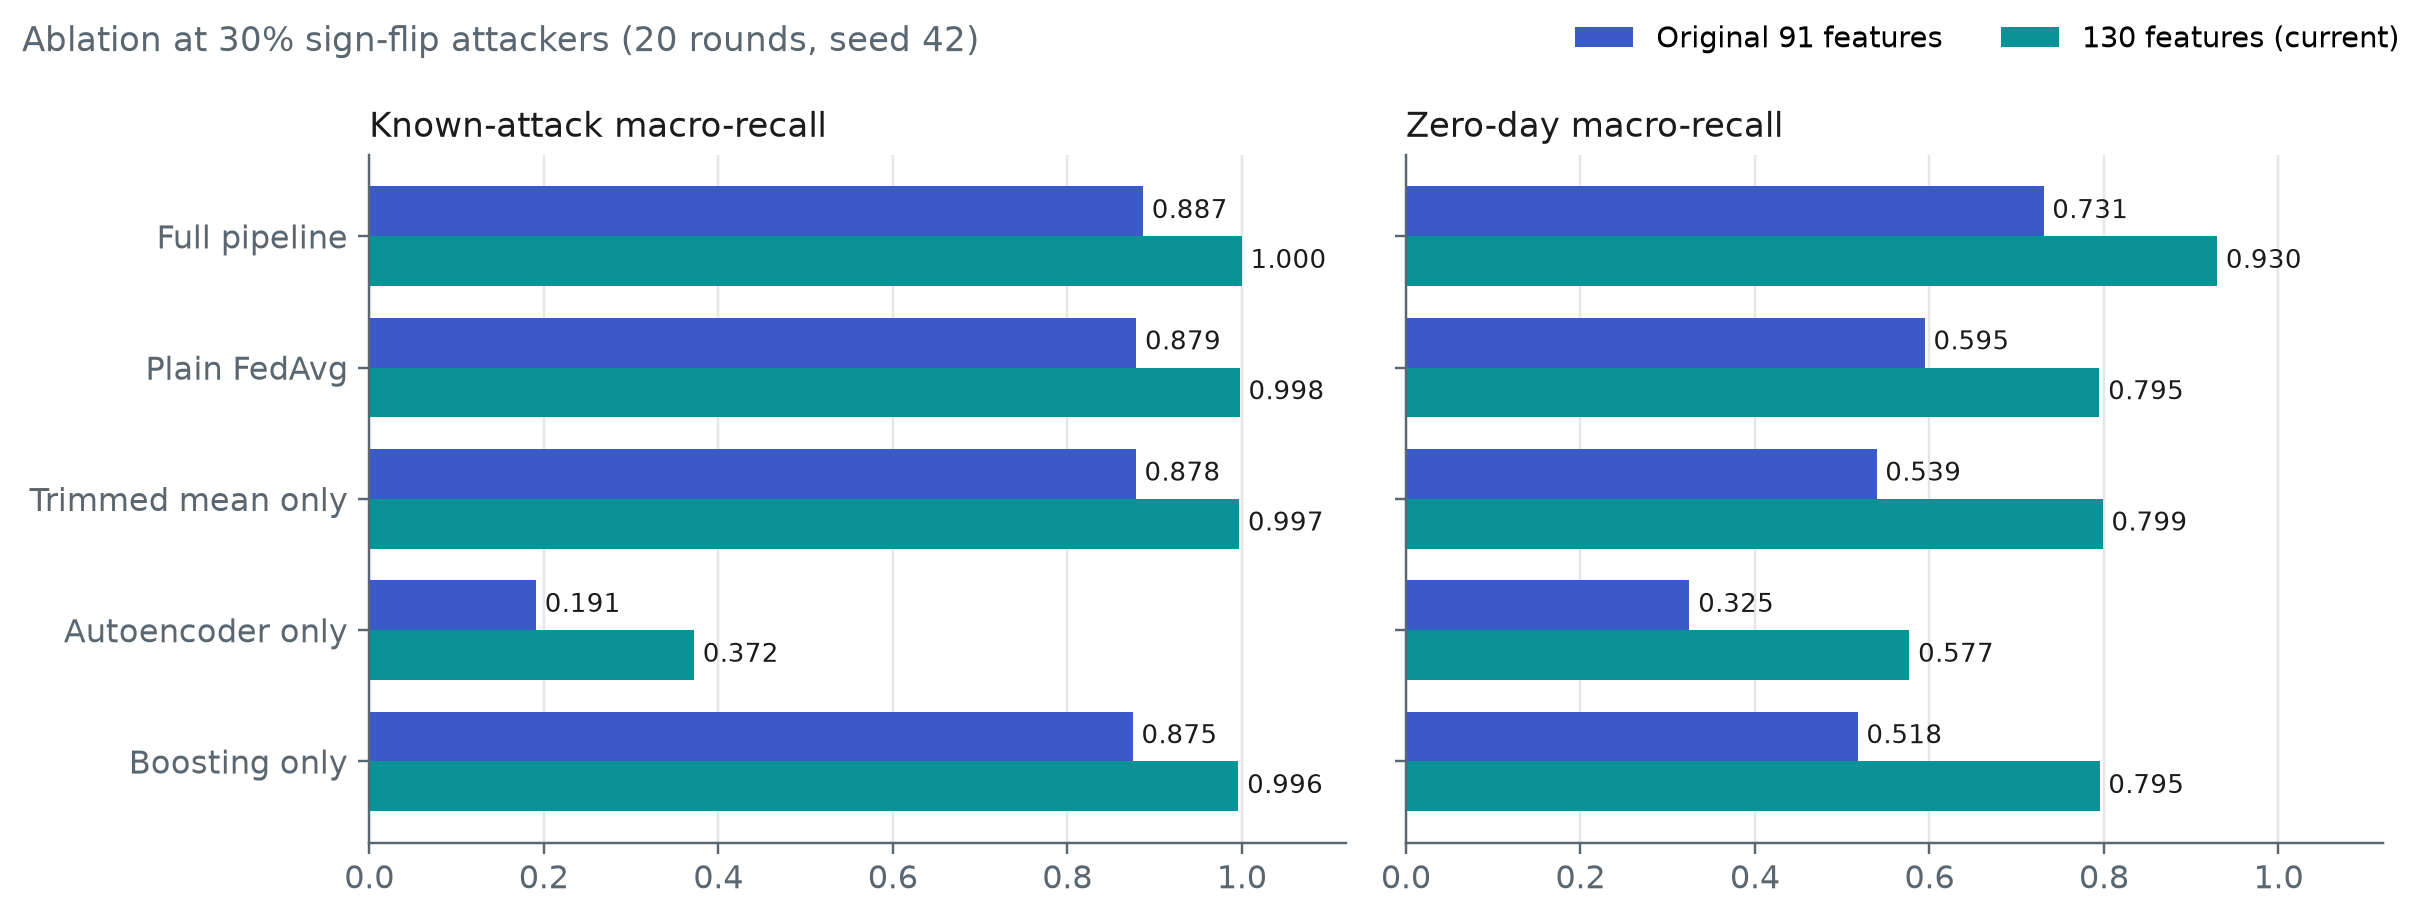
\includegraphics[width=\linewidth]{figures/ablation.png}
\caption{Ablation: known-attack and zero-day macro-recall, original vs.\ current features}
\label{fig:ablation}
\end{figure}
One trade-off is worth stating. On known attacks, boosting alone now has a higher detection F1 than the full cascade (0.998 vs.\ 0.961). The autoencoder's threshold is set to flag about 3\% of benign traffic, and that cost now outweighs the little it adds when the classifier already catches 99.6\% of known attacks. Final validation losses: full pipeline 0.028; plain FedAvg $5.0\times10^{20}$ and trimmed mean $1.3\times10^{4}$ (diverged). Communication: 15.7\,MB over 20 rounds (the autoencoder now has 9{,}834 parameters, up from 7{,}299).

\subsubsection{Poisoning resistance}
Figure~\ref{fig:poison} sweeps the share of sign-flip attackers from 0 to 50\%. Attack macro-recall stays between 0.997 and 1.000 at every fraction [0.878--0.887], and zero-day macro-recall between 0.901 and 0.943 up to 40\% [0.724--0.736]. Attackers got past the filter in 10\%, 12\% and 36\% of attacker-rounds at 20\%, 30\% and 40\% [28\%, 32\%, 24\%]: lower at the first two fractions but higher at 40\%, although the autoencoder still held there (stand-alone recall 0.691). At 50\% the coordinate-wise median reference becomes the attackers' direction again: every attacker update passes, the autoencoder collapses, and zero-day detection falls back to the classifier (0.803). This is the known limit of median-based defences~\cite{yin2018trimmed}. A repeat with seeds 43 and 44 at 20\% and 30\% gave 0.996--0.999 attack macro-recall for every seed, while stand-alone autoencoder recall varied by seed (0.56--0.74), as it did with the original features.
\begin{figure}[H]
\centering
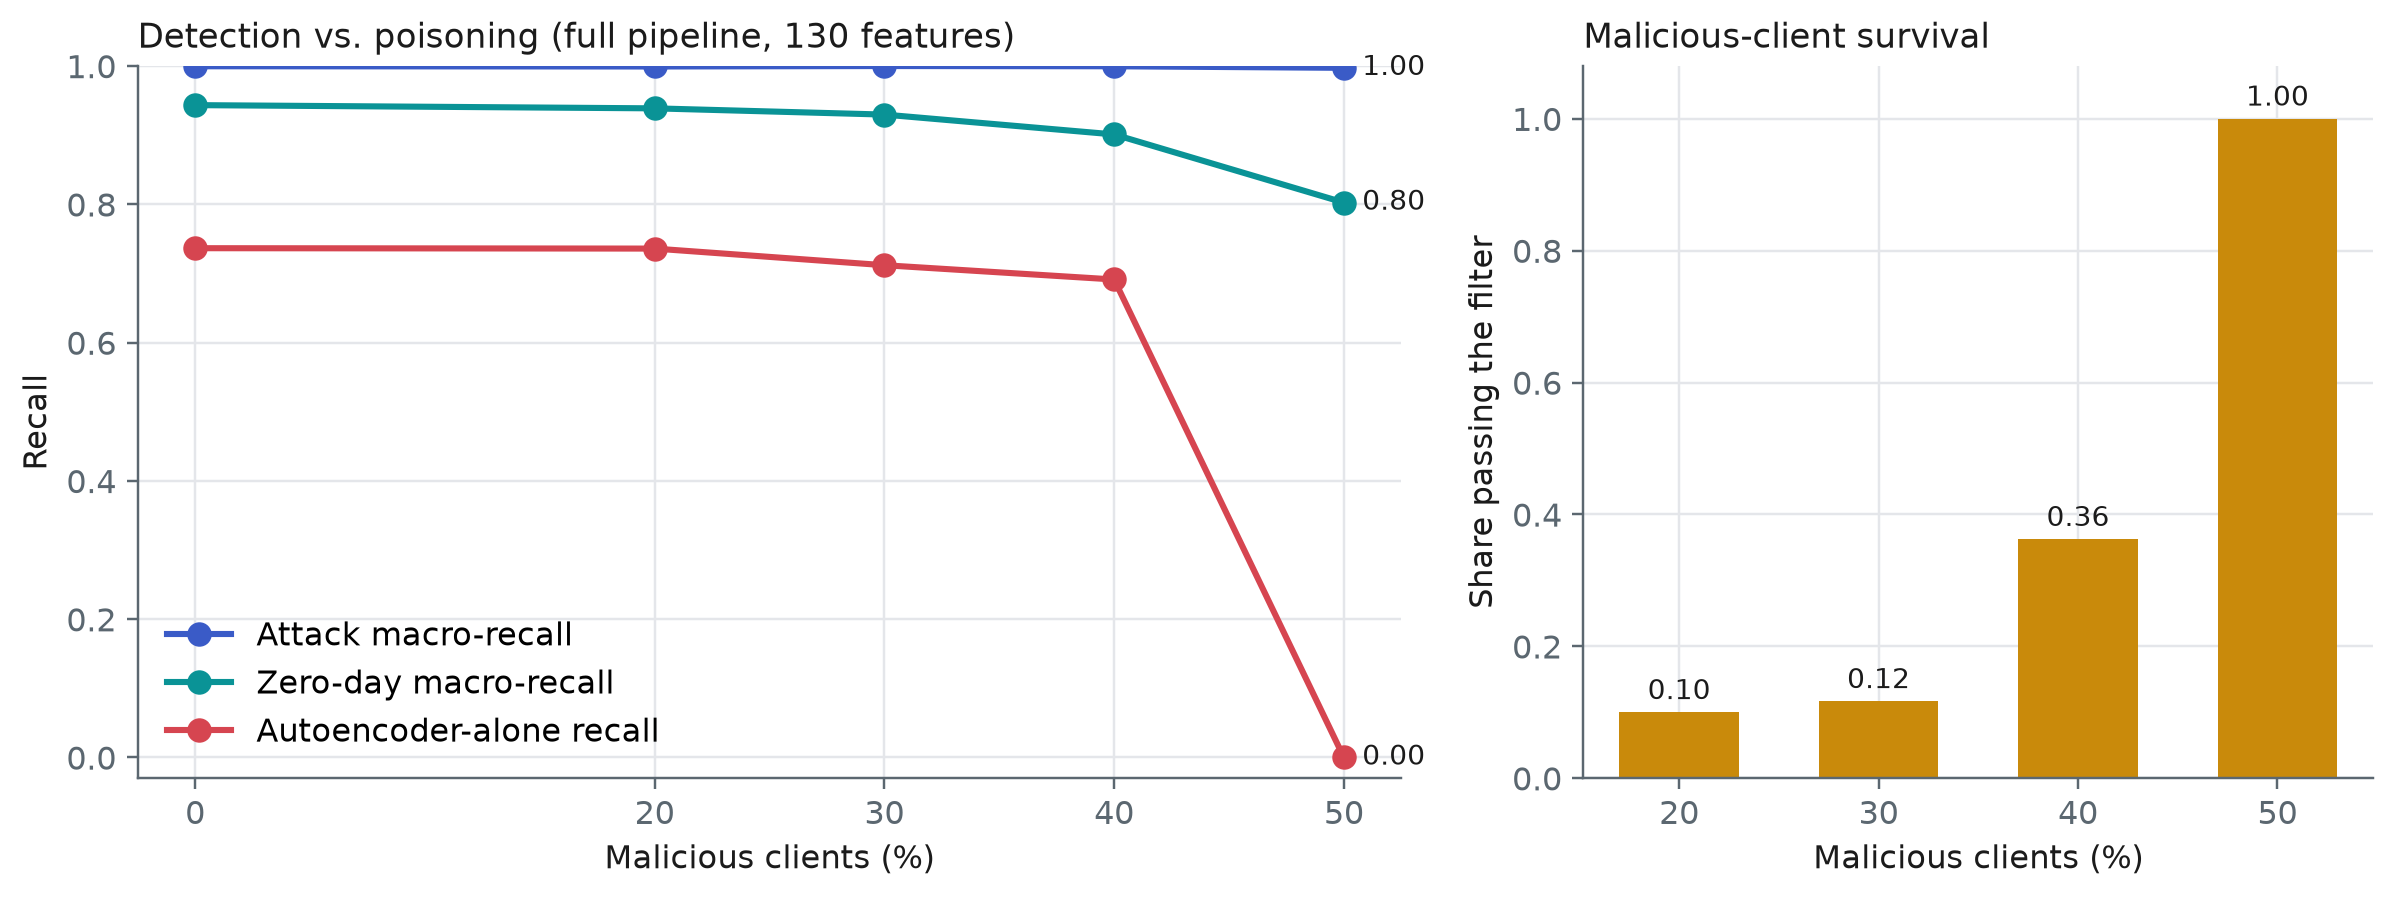
\includegraphics[width=\linewidth]{figures/poisoning_sweep.png}
\caption{Detection and malicious-client survival vs.\ share of malicious clients (130 features)}
\label{fig:poison}
\end{figure}

\subsubsection{Zero-day detection}
Each of the 14 attack classes was removed in turn from all training data (including scaler statistics) and then scored as unseen traffic (Figures~\ref{fig:zeroday} and~\ref{fig:zerodaycmp}). The cascade's average detection rose from 0.736 to \textbf{0.943}; boosting alone from 0.533 to 0.801 and the autoencoder alone from 0.493 to 0.757. The autoencoder separates unseen attacks from benign traffic far better than before (AUROC 0.968--1.000 for every class, against 0.59--0.70 for the HTTP-family attacks with the original features). The largest gains are on the attacks that were hardest before: Password 0.44$\rightarrow$0.97, Ransomware 0.54$\rightarrow$1.00, SQL\_injection 0.61$\rightarrow$1.00, XSS 0.52$\rightarrow$0.99 and DDoS\_HTTP 0.36$\rightarrow$0.88.

Two classes got worse and are reported rather than hidden. MITM fell from 0.89 to 0.69: its single ARP connection gets ordinary-looking connection features, so the autoencoder finds it less unusual. Unseen Uploading traffic now looks normal to the classifier (boosting-only 0.49$\rightarrow$0.08); the autoencoder catches most of it, so the cascade still improves (0.52$\rightarrow$0.72). The benign false-positive rate stays about 3\%, as set by the 97th-percentile threshold.
\begin{figure}[H]
\centering
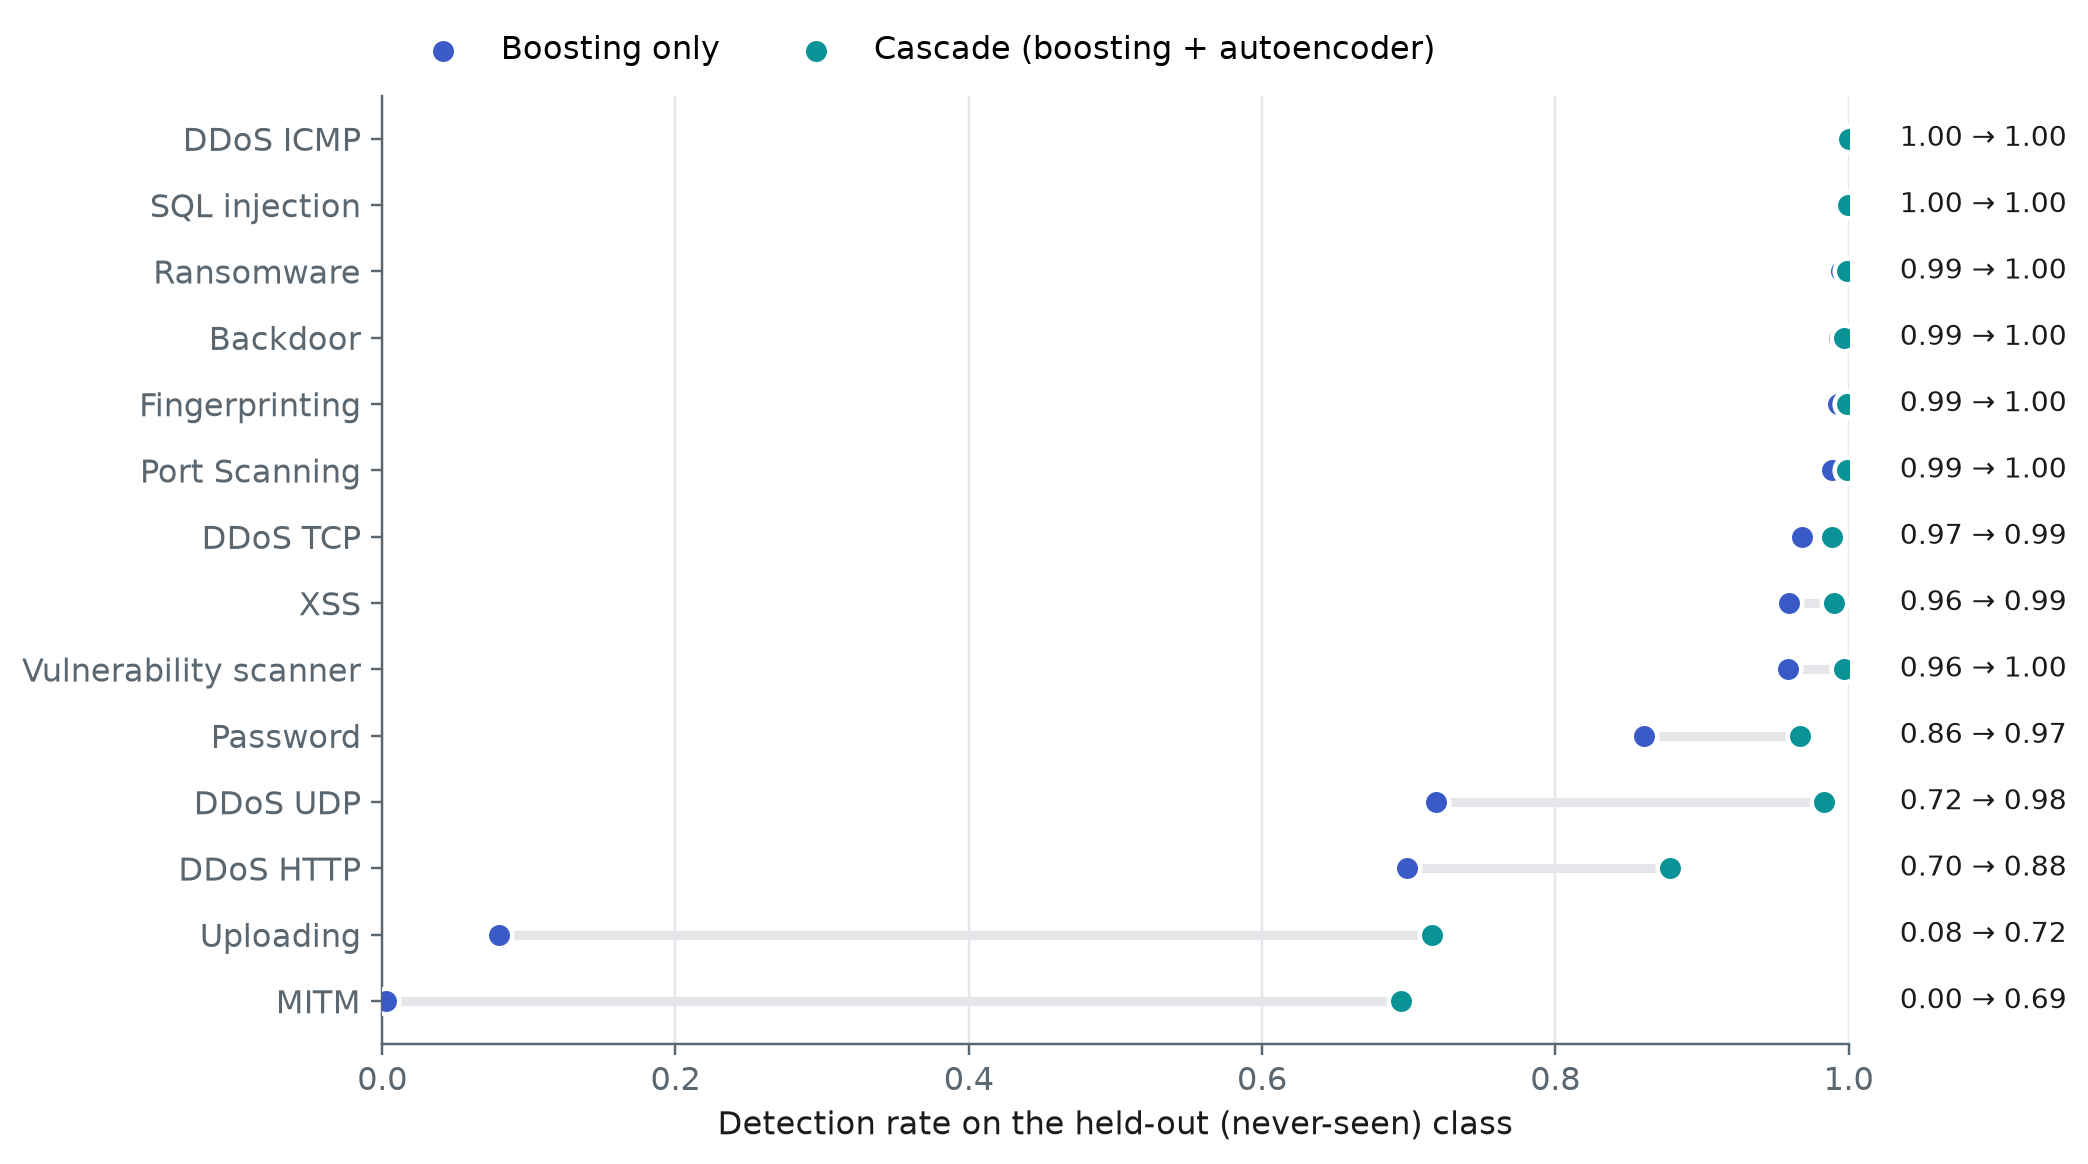
\includegraphics[width=0.88\linewidth]{figures/zero_day.png}
\caption{Zero-day detection per held-out class: boosting alone vs.\ cascade (130 features)}
\label{fig:zeroday}
\end{figure}
\begin{figure}[H]
\centering
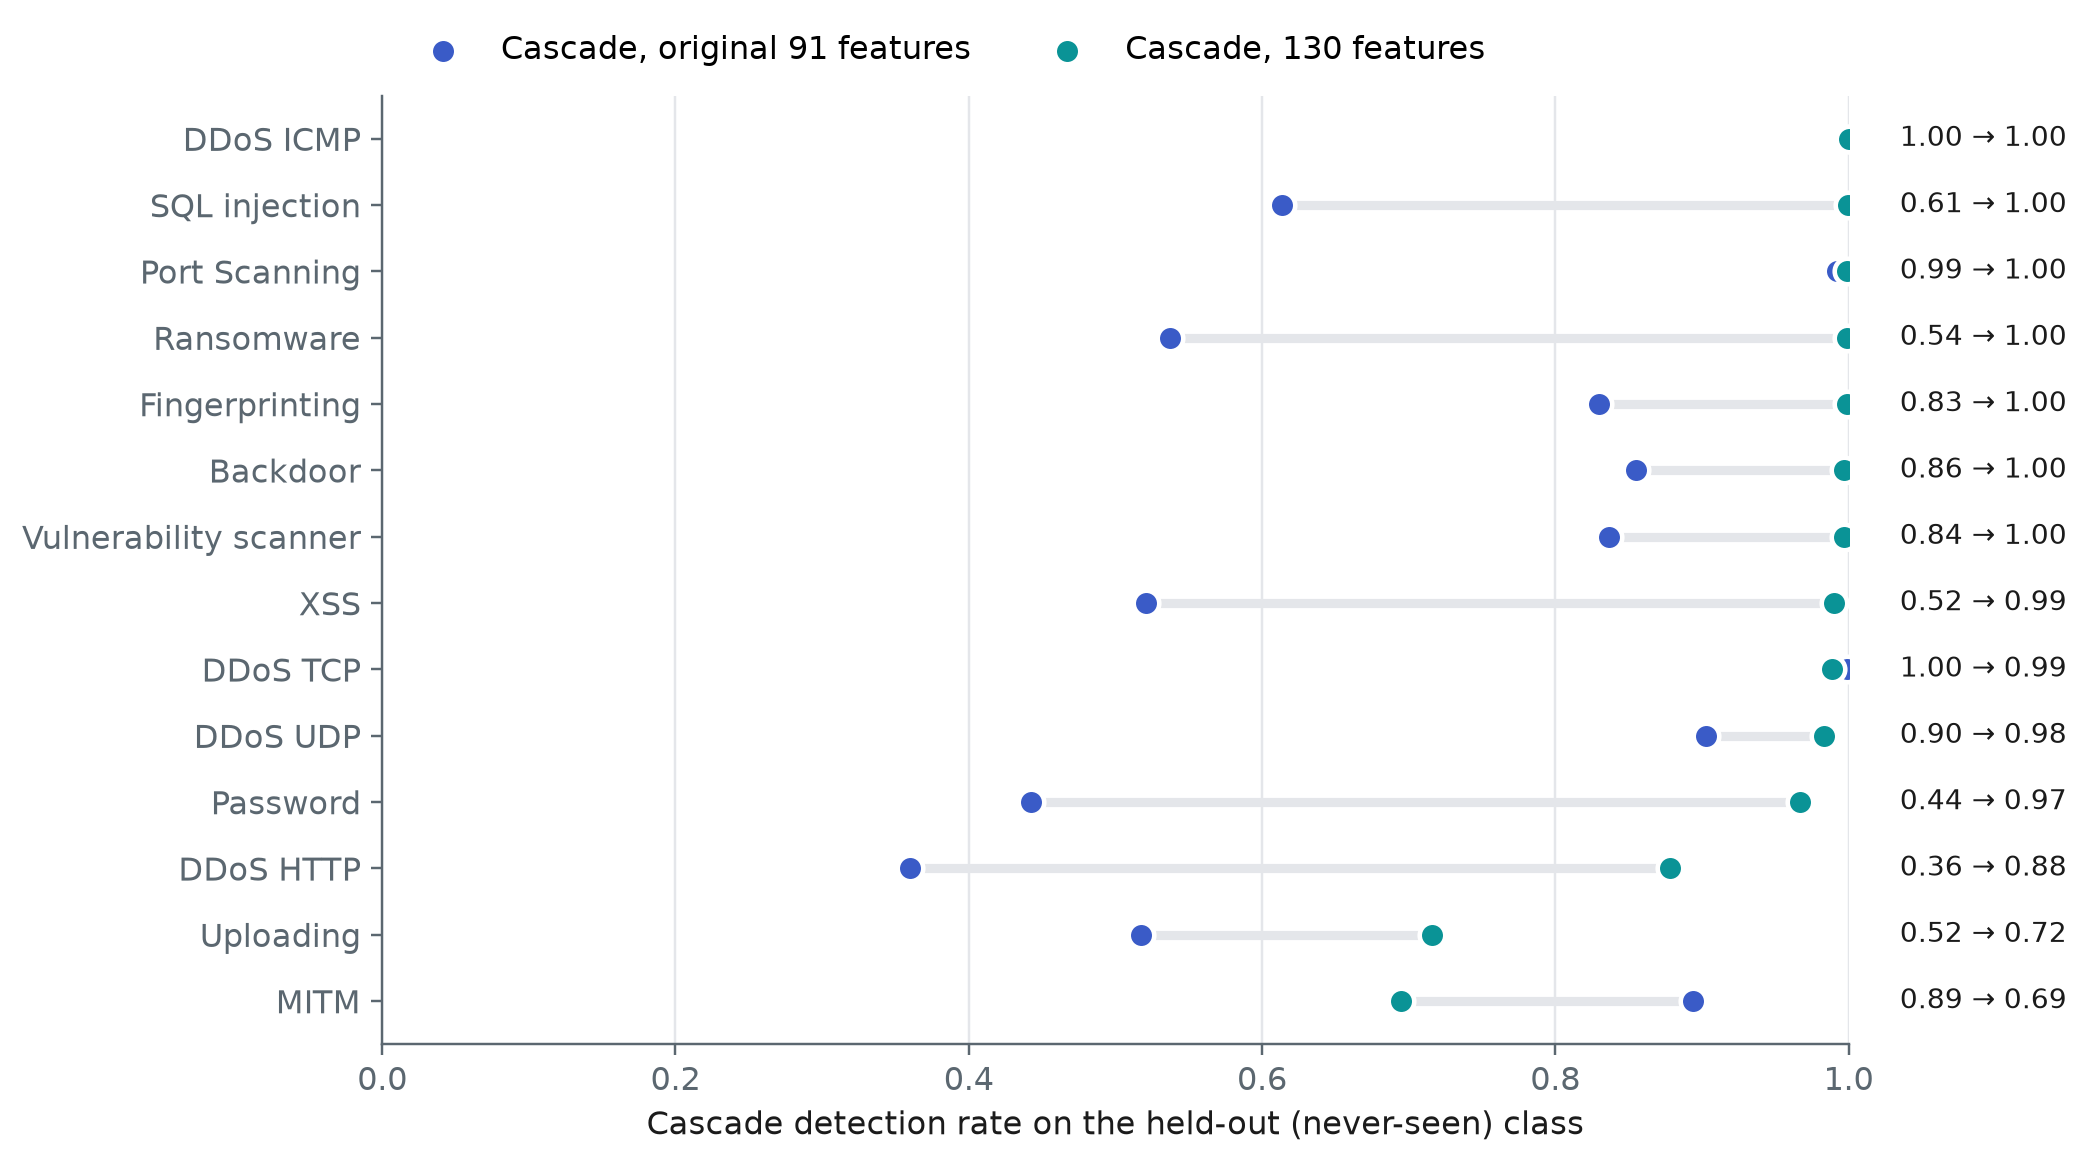
\includegraphics[width=0.88\linewidth]{figures/zero_day_compare.png}
\caption{Cascade zero-day detection per held-out class: original 91 features vs.\ 130 features}
\label{fig:zerodaycmp}
\end{figure}

\subsubsection{Real multi-process run and SDN mitigation}
\textbf{Phase A, real run.} A real Flower server and 10 separate client processes completed 20 rounds in about 4 minutes. The bootstrap classifier reached 0.997 accuracy on the calibration hold-out [0.963]. The final cascade gave \textbf{0.999} attack macro-recall [0.889] and a 0.035 benign false-positive rate [0.035] on the clients' test slices. A separate full-pipeline run scored per class gave 0.976 accuracy and 0.971 macro F1 for the cascade [0.944 / 0.931], and an autoencoder AUROC of 0.982 [0.805].

\textbf{Phase B.} Live extraction now derives the same 130 features from the capture with the same code as training: for \texttt{Backdoor\_attack.pcap}, 99.8\% of the live rows are identical to that capture's training rows. Replayed through Mininet with the new bundle, the capture was classified as \textbf{Backdoor with 0.997 confidence} by the boosting stage, 24{,}669 of its 24{,}914 packets were flagged [23{,}895], the bridge chose \emph{block}, and the rule \texttt{priority=100,ip,nw\_src=10.0.0.1 actions=drop} was confirmed in the switch's flow table. Because classification happens once features have been extracted from the whole capture, 23{,}161 replayed packets had already been forwarded when the rule appeared. The mitigation is therefore capture-level, not inline per-packet blocking.

\subsubsection{Scaling to 20 clients, repeat seeds and run timing}
\textbf{Real 20-process runs.} The project was re-hosted on a virtual machine with 24~GB of memory, which can hold one Flower server and 20 client processes (an earlier attempt on a 7.4~GB machine could not). Phase A was run with 10 and with 20 real client processes at seeds 42, 43 and 44 (20 rounds, no attackers). The seed changes the data split, the Dirichlet partition and the initialisation. Table~\ref{tab:realruns} lists every run. Over the three seeds the cascade's attack macro-recall averages 0.998 with 10 clients and 0.992 with 20 clients, and the benign false-positive rate stays between 2.8\% and 4.0\%. At seed 42, the 20-client run dips to 0.978; this run was not analysed per class, so its cause is not established. With only three seeds, no confidence intervals are claimed.

\begin{table}[H]
\centering
\renewcommand{\arraystretch}{1.2}
\begin{tabular}{|l|c|c|c|c|}
\hline
\textbf{Run} & \textbf{Phase A (s)} & \textbf{Attack macro-recall} & \textbf{False alarms} & \textbf{Classifier acc.} \\ \hline
10 clients, seed 42 & 341 & 0.999 & 3.40\% & 0.9969 \\ \hline
10 clients, seed 43 & 276 & 0.999 & 3.11\% & 0.9976 \\ \hline
10 clients, seed 44 & 262 & 0.996 & 2.84\% & 0.9968 \\ \hline
20 clients, seed 42 & 247 & 0.978 & 3.62\% & 0.9969 \\ \hline
20 clients, seed 43 & 238 & 0.999 & 2.84\% & 0.9976 \\ \hline
20 clients, seed 44 & 242 & 0.999 & 3.96\% & 0.9968 \\ \hline
\end{tabular}
\caption{Real multi-process Phase A runs (source: \texttt{results/real\_runs/summary.md})}
\label{tab:realruns}
\end{table}

Phase B on the 20-client bundle classified \texttt{Backdoor\_attack.pcap} as Backdoor with 0.997 confidence, flagged 24{,}466 of 24{,}914 packets, and the drop rule \texttt{priority=100,ip,nw\_src=10.0.0.1 actions=drop} was read back from the switch.

\textbf{The trust filter without attackers.} Even with no malicious clients, the filter excluded some clients' updates: over 20 rounds, 15, 2 and 6 client-rounds with 10 clients, and 38, 42 and 27 with 20 clients (seeds 42, 43, 44). These are honest clients whose non-IID updates look unlike the median, so the filter cannot tell unusual data from sabotage. This is the confound named in the limitations, and it is more frequent with 20 clients.

\textbf{Simulation versus real run.} An in-process simulation of 20 clients (seed 42) gave a cascade attack-detection recall of 0.9960 against 0.9996 for 10 clients, an autoencoder recall of 0.685 against 0.728, and benign false alarms of 3.72\% against 3.32\%. Three of the 20 simulated clients received no benign validation rows, so their anomaly threshold is infinite and their autoencoder never flags. The simulation uses the same client, strategy and trust-filter code as the real run, and the table above is the real-process evidence.

\textbf{Timing of one complete run.} One real run (10 client processes, warm feature cache) took 219~s in total: Phase A 210.6~s, of which federated training was 191.2~s, and Phase B 8.6~s. Tables~\ref{tab:timea} and~\ref{tab:timeb} give the stages.

\begin{table}[H]
\centering
\renewcommand{\arraystretch}{1.2}
\begin{tabular}{|l|c|}
\hline
\textbf{Phase A stage} & \textbf{Seconds} \\ \hline
Load, clean and encode the dataset & 1.9 \\ \hline
Calibration split, bootstrap classifier, client partition & 14.4 \\ \hline
Federated training & 191.2 \\ \hline
Calibrate client anomaly thresholds & 0.1 \\ \hline
Evaluate on the clients' test slices & 2.5 \\ \hline
Save the model bundle & 0.2 \\ \hline
\end{tabular}
\caption{Phase A stage timing (source: \texttt{results/journey/phase\_a\_journey.json})}
\label{tab:timea}
\end{table}

\begin{table}[H]
\centering
\renewcommand{\arraystretch}{1.2}
\begin{tabular}{|l|c|}
\hline
\textbf{Phase B stage} & \textbf{Seconds} \\ \hline
Load the model bundle & 0.08 \\ \hline
Start the SDN bridge and controller & 2.20 \\ \hline
Network, replay, classify and block (root process) & 6.33 \\ \hline
Check the switch's flow table & 0.00 \\ \hline
\end{tabular}
\caption{Phase B stage timing (source: \texttt{results/journey/phase\_b\_journey.json})}
\label{tab:timeb}
\end{table}

\subsubsection{Follow-up experiments: more seeds, an adaptive attacker, pruning and a time-ordered split}\label{sec:followups}
These experiments were run after the main results, in the virtual machine, and every table is generated from the experiments' own result files.

\textbf{More seeds.} The ablation, the poisoning sweep and the zero-day experiment were repeated at seeds 43 and 44 (Tables~\ref{tab:fu_seed_ablation}--\ref{tab:fu_seed_zeroday}). The conclusions hold in all three seeds: the full pipeline's attack macro-recall stays between 0.995 and 1.000 up to 50\% attackers; plain FedAvg and the trimmed mean alone leave the autoencoder at recall 0.000--0.026 with 30\% attackers; the trust filter fails at 50\% (attacker survival 0.97--1.00); and the cascade's mean zero-day detection is 0.943, 0.952 and 0.952. Other numbers move with the seed: the autoencoder's recall at 30\% attackers ranges from 0.565 to 0.712, attacker survival at 20\% from 0.03 to 0.23, and MITM zero-day detection from 0.695 to 0.963. The per-class zero-day columns inside the ablation and sweep tables were not repeated at seeds 43 and 44 (about 85 extra trainings per seed). Three seeds are too few for confidence intervals.

\begin{table}[H]
\centering
\small
\setlength{\tabcolsep}{3pt}
\renewcommand{\arraystretch}{1.15}
\begin{tabular}{|l|c|c|c|}
\hline
\textbf{Variant} & \textbf{Attack macro-recall} & \textbf{Autoencoder-alone recall} & \textbf{Benign FPR} \\ \hline
full\_pipeline & 1.000 / 0.999 / 0.997 & 0.712 / 0.679 / 0.565 & 0.0309 / 0.0284 / 0.0320 \\ \hline
plain\_fedavg & 0.998 / 0.997 / 0.994 & 0.002 / 0.000 / 0.000 & 0.0347 / 0.0317 / 0.0297 \\ \hline
trimmed\_mean\_only & 0.997 / 0.997 / 0.996 & 0.000 / 0.000 / 0.026 & 0.0334 / 0.0291 / 0.0337 \\ \hline
autoencoder\_only & 0.372 / 0.295 / 0.306 & 0.372 / 0.295 / 0.306 & 0.0301 / 0.0281 / 0.0325 \\ \hline
boosting\_only & 0.996 / 0.997 / 0.996 & n/a / n/a / n/a & 0.0002 / 0.0000 / 0.0005 \\ \hline
\end{tabular}
\caption{Ablation at 30\% sign-flip attackers, seeds 42 / 43 / 44 (source: results/seeds/summary.json)}
\label{tab:fu_seed_ablation}
\end{table}
\begin{table}[H]
\centering
\small
\setlength{\tabcolsep}{3pt}
\renewcommand{\arraystretch}{1.15}
\begin{tabular}{|l|c|c|c|}
\hline
\textbf{Attackers} & \textbf{Attack macro-recall} & \textbf{Autoencoder-alone recall} & \textbf{Attacker survival} \\ \hline
0\% & 1.000 / 0.999 / 0.997 & 0.737 / 0.765 / 0.612 & n/a / n/a / n/a \\ \hline
20\% & 0.999 / 0.999 / 0.996 & 0.736 / 0.739 / 0.618 & 0.10 / 0.03 / 0.23 \\ \hline
30\% & 1.000 / 0.999 / 0.997 & 0.712 / 0.679 / 0.565 & 0.12 / 0.12 / 0.27 \\ \hline
40\% & 1.000 / 0.998 / 0.997 & 0.691 / 0.620 / 0.537 & 0.36 / 0.31 / 0.44 \\ \hline
50\% & 0.997 / 0.997 / 0.995 & 0.000 / 0.000 / 0.000 & 1.00 / 0.99 / 0.97 \\ \hline
\end{tabular}
\caption{Poisoning sweep, seeds 42 / 43 / 44}
\label{tab:fu_seed_sweep}
\end{table}
\begin{table}[H]
\centering
\small
\setlength{\tabcolsep}{3pt}
\renewcommand{\arraystretch}{1.15}
\begin{tabular}{|l|c|}
\hline
\textbf{Stage} & \textbf{Mean detection rate} \\ \hline
Classifier alone & 0.801 / 0.748 / 0.791 \\ \hline
Autoencoder alone & 0.757 / 0.775 / 0.747 \\ \hline
Cascade & 0.943 / 0.952 / 0.952 \\ \hline
Cascade, DDoS\_HTTP & 0.878 / 0.846 / 0.948 \\ \hline
Cascade, MITM & 0.695 / 0.963 / 0.837 \\ \hline
Cascade, Uploading & 0.716 / 0.677 / 0.665 \\ \hline
\end{tabular}
\caption{Zero-day detection of the unseen class, mean over 14 classes, seeds 42 / 43 / 44}
\label{tab:fu_seed_zeroday}
\end{table}
\textbf{Why the 20-client run dipped.} The seed-42 run with 20 real clients scored attack macro-recall 0.978, against 0.996--0.999 elsewhere. The cause is one missed Fingerprinting test row out of four; micro recall is 0.9964 (Table~\ref{tab:fu_realrun_breakdown}). Clients without benign validation rows (infinite threshold) were still caught by the classifier.

\begin{table}[H]
\centering
\scriptsize
\setlength{\tabcolsep}{3pt}
\renewcommand{\arraystretch}{1.15}
\begin{tabular}{|l|c|c|c|c|c|}
\hline
\textbf{Run} & \textbf{Macro-recall} & \textbf{Micro recall} & \textbf{Fingerprinting test rows, recall} & \textbf{MITM test rows, recall} & \textbf{Clients with infinite threshold} \\ \hline
10 clients, seed 42 & 0.999 & 0.9992 & 3 rows, 1.00 & 3 rows, 1.00 & 0 \\ \hline
10 clients, seed 43 & 0.999 & 0.9992 & 4 rows, 1.00 & 4 rows, 1.00 & 1 \\ \hline
10 clients, seed 44 & 0.996 & 0.9960 & 4 rows, 1.00 & 5 rows, 1.00 & 1 \\ \hline
20 clients, seed 42 & 0.978 & 0.9964 & 4 rows, 0.75 & 1 rows, 1.00 & 3 \\ \hline
20 clients, seed 43 & 0.999 & 0.9992 & 2 rows, 1.00 & 3 rows, 1.00 & 2 \\ \hline
20 clients, seed 44 & 0.999 & 0.9988 & 2 rows, 1.00 & 3 rows, 1.00 & 2 \\ \hline
\end{tabular}
\caption{Where the real-run macro-recall comes from (source: results/real\_runs/<run>/, made by fl\_ids.eval.bundle\_report)}
\label{tab:fu_realrun_breakdown}
\end{table}
\textbf{Real attackers.} With sign-flip attackers in the real multi-process run, the trust filter excluded the attackers' updates in 36 of 40 (20\%) and 52 of 60 (30\%) client-rounds, and excluded no honest client (Table~\ref{tab:fu_attack_runs}, Figure~\ref{fig:trustmal03}).

\begin{table}[H]
\centering
\scriptsize
\setlength{\tabcolsep}{3pt}
\renewcommand{\arraystretch}{1.15}
\begin{tabular}{|l|c|c|c|c|c|}
\hline
\textbf{Attackers} & \textbf{Attacker clients} & \textbf{Attacker client-rounds excluded} & \textbf{Honest client-rounds excluded} & \textbf{Attack macro-recall} & \textbf{Benign FPR} \\ \hline
20\% & 0,7 & 36 of 40 & 0 of 160 & 0.998 & 0.0335 \\ \hline
30\% & 0,6,9 & 52 of 60 & 0 of 140 & 0.999 & 0.0317 \\ \hline
\end{tabular}
\caption{Real multi-process Phase A with sign-flip attackers (10 clients, 20 rounds, seed 42; source: runs/attack\_runs/)}
\label{tab:fu_attack_runs}
\end{table}
\begin{figure}[H]
\centering
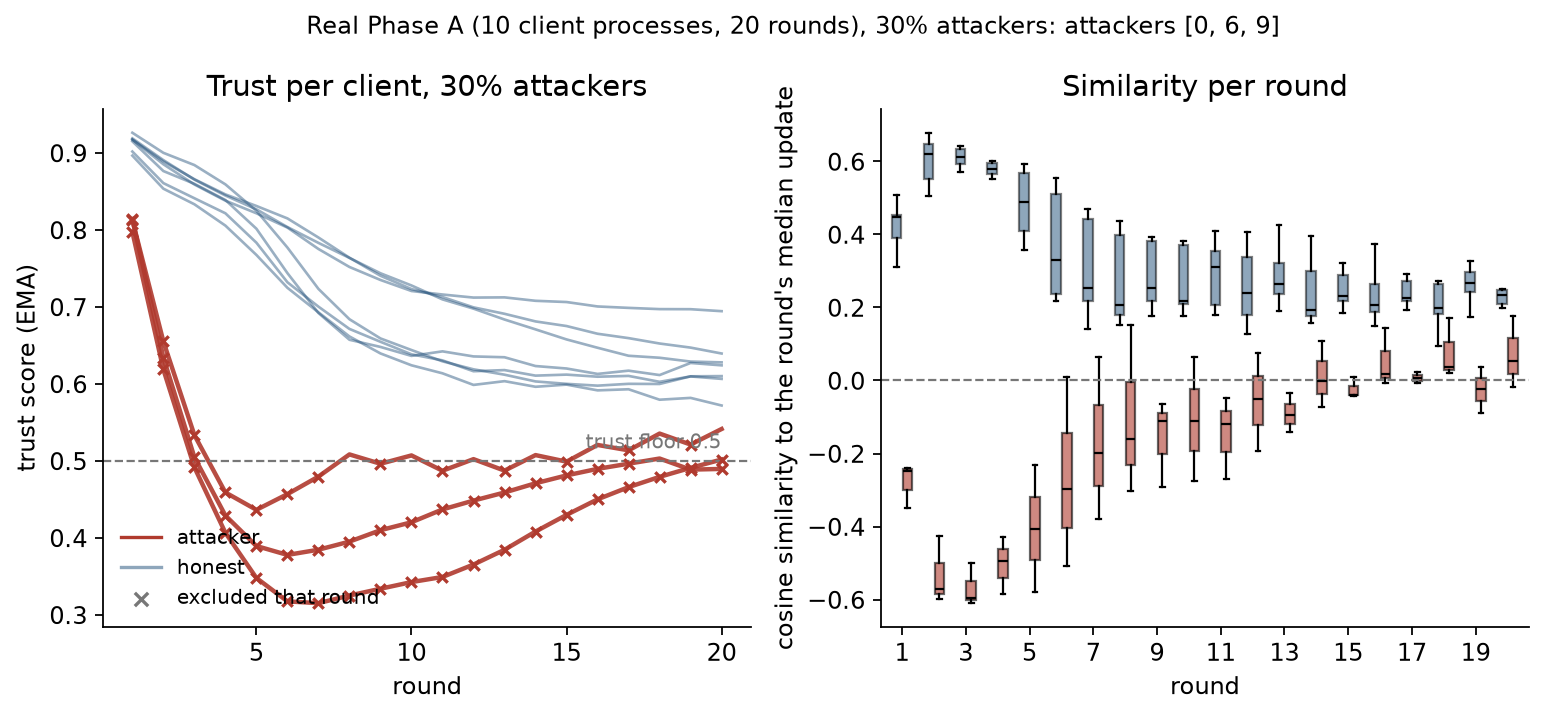
\includegraphics[width=0.98\linewidth]{figures/trust_mal03.png}
\caption{Real run with 30\% sign-flip attackers: trust score (left) and cosine similarity to the round's median update (right)}
\label{fig:trustmal03}
\end{figure}
\textbf{An adaptive attacker.} A white-box attacker that knows the filter's rule estimates the consensus from the last aggregate update, keeps a cosine similarity of 0.1 to it, and spends the rest of a norm budget (1.5 times its honest norm, under the clip) on the opposite of its honest update's orthogonal component. The filter mostly fails against it: attackers survive in 72--90\% of client-rounds instead of 10--36\% (Table~\ref{tab:fu_adaptive}). The damage is bounded: known-attack recall stays at 0.9997 or above, but the autoencoder's recall alone falls to 0.499 at 40\% attackers (0.663 for sign-flip). Zero-day detection under this attacker was not measured, and this is one adaptive strategy, not a proof for all.

\begin{table}[H]
\centering
\scriptsize
\setlength{\tabcolsep}{3pt}
\renewcommand{\arraystretch}{1.15}
\begin{tabular}{|l|c|c|c|c|c|}
\hline
\textbf{Attack} & \textbf{Attackers} & \textbf{Attack macro-recall} & \textbf{Autoencoder-alone recall} & \textbf{Attacker survival} & \textbf{Final validation loss} \\ \hline
sign\_flip & 20\% & 0.9993 & 0.730 & 0.10 & 0.026 \\ \hline
sign\_flip & 30\% & 1.0000 & 0.718 & 0.12 & 0.029 \\ \hline
sign\_flip & 40\% & 0.9997 & 0.663 & 0.36 & 0.021 \\ \hline
stealth & 20\% & 0.9997 & 0.747 & 0.90 & 0.041 \\ \hline
stealth & 30\% & 1.0000 & 0.741 & 0.72 & 0.040 \\ \hline
stealth & 40\% & 0.9997 & 0.499 & 0.82 & 0.037 \\ \hline
\end{tabular}
\caption{Adaptive (stealth) attacker vs. sign-flip, seed 42, 20 rounds (source: results/adaptive/adaptive\_attack.csv)}
\label{tab:fu_adaptive}
\end{table}
\textbf{Weight pruning (Objective 3).} The autoencoder's weight matrices were magnitude-pruned after training and during federated training (the server re-prunes every round). Pruning after training damages the backstop at once, while pruning during training keeps it up to about 70\% sparsity: autoencoder-alone recall 0.744 dense, 0.727 at 50\%, 0.688 at 70\%, then 0.467 at 80\% (Tables~\ref{tab:fu_prune_post} and~\ref{tab:fu_prune_fl}). A sparse layout needs index storage, so the size falls below the dense size only past 50\% sparsity (0.61 of the dense bytes at 70\%; computed from the non-zero counts, not transmitted). Clients still send dense updates, so this reduces the model, not the per-round communication. Single seed, no attackers.

\begin{table}[H]
\centering
\scriptsize
\setlength{\tabcolsep}{3pt}
\renewcommand{\arraystretch}{1.15}
\begin{tabular}{|l|c|c|c|c|c|c|}
\hline
\textbf{Sparsity} & \textbf{Non-zero weights} & \textbf{Sparse / dense bytes} & \textbf{Autoencoder recall} & \textbf{Autoencoder AUROC} & \textbf{Cascade macro-recall} & \textbf{Benign FPR} \\ \hline
0\% & 9600 & 1.98 & 0.742 & 0.987 & 0.999 & 0.0340 \\ \hline
50\% & 4800 & 1.00 & 0.273 & 0.742 & 0.998 & 0.0287 \\ \hline
70\% & 2880 & 0.61 & 0.168 & 0.596 & 0.998 & 0.0292 \\ \hline
80\% & 1920 & 0.41 & 0.145 & 0.559 & 0.996 & 0.0334 \\ \hline
90\% & 960 & 0.22 & 0.144 & 0.594 & 0.996 & 0.0323 \\ \hline
95\% & 480 & 0.12 & 0.147 & 0.593 & 0.996 & 0.0366 \\ \hline
98\% & 192 & 0.06 & 0.147 & 0.593 & 0.996 & 0.0366 \\ \hline
\end{tabular}
\caption{Post-training magnitude pruning of the 10-client autoencoder, thresholds recalibrated (source: results/pruning/c10\_s42/pruning.csv)}
\label{tab:fu_prune_post}
\end{table}
\begin{table}[H]
\centering
\scriptsize
\setlength{\tabcolsep}{3pt}
\renewcommand{\arraystretch}{1.15}
\begin{tabular}{|l|c|c|c|c|c|c|}
\hline
\textbf{Sparsity} & \textbf{Non-zero weights} & \textbf{Sparse / dense bytes} & \textbf{Autoencoder-alone recall} & \textbf{Cascade macro-recall} & \textbf{Benign FPR} & \textbf{Final validation loss} \\ \hline
0\% & 9600 & 1.98 & 0.744 & 1.000 & 0.0320 & 0.034 \\ \hline
50\% & 4800 & 1.00 & 0.727 & 1.000 & 0.0323 & 0.040 \\ \hline
70\% & 2880 & 0.61 & 0.688 & 1.000 & 0.0298 & 0.049 \\ \hline
80\% & 1920 & 0.41 & 0.467 & 0.999 & 0.0312 & 0.080 \\ \hline
90\% & 960 & 0.22 & 0.176 & 0.998 & 0.0289 & 0.207 \\ \hline
\end{tabular}
\caption{Pruning during federated training (server re-prunes each round, linear ramp over the first 10 rounds), seed 42, no attackers (source: results/pruning/pruning\_during\_fl.csv)}
\label{tab:fu_prune_fl}
\end{table}
\textbf{Clipping.} Without the per-client z-score clip the benign validation loss stays near 50; with it, it falls from 0.2047 to 0.03369 (Table~\ref{tab:fu_clip}, Figure~\ref{fig:clipval}).

\begin{table}[H]
\centering
\scriptsize
\setlength{\tabcolsep}{3pt}
\renewcommand{\arraystretch}{1.15}
\begin{tabular}{|l|c|c|c|c|}
\hline
\textbf{Normalisation} & \textbf{Round 1} & \textbf{Round 5} & \textbf{Round 10} & \textbf{Round 20} \\ \hline
clip 10 & 0.2047 & 0.04336 & 0.03999 & 0.03369 \\ \hline
no clip & 50.63 & 50.15 & 50 & 49.86 \\ \hline
\end{tabular}
\caption{Benign validation loss with and without the per-client z-score clip (source: results/clip/clip\_comparison.csv)}
\label{tab:fu_clip}
\end{table}
\begin{figure}[H]
\centering
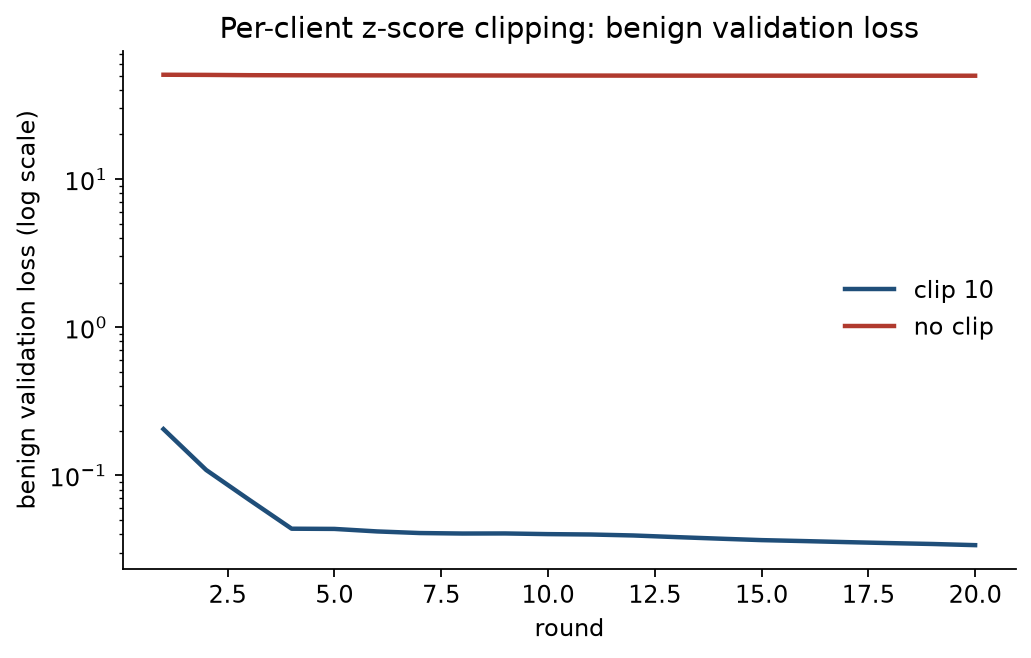
\includegraphics[width=0.7\linewidth]{figures/clip_val_loss.png}
\caption{Benign validation loss with and without the per-client z-score clip}
\label{fig:clipval}
\end{figure}
\textbf{A time-ordered split.} Each class's earliest 80\% of connections were used for training and its latest 20\% for testing (the CSV is in capture order within a class, but its timestamps carry no date, so this orders by row position). Accuracy is 0.994 against 0.997 for the connection-grouped split (Table~\ref{tab:fu_temporal_summary}). Macro F1 falls from 0.983 to 0.913, mostly because MITM is a single connection, so it falls entirely in the test side and enters the mean with recall 0; without it the figure is about 0.978. The real losses are Backdoor (0.989 to 0.947--0.962) and DDoS\_HTTP (0.980 to 0.912--0.925).

\begin{table}[H]
\centering
\small
\setlength{\tabcolsep}{3pt}
\renewcommand{\arraystretch}{1.15}
\begin{tabular}{|l|c|c|}
\hline
\textbf{Split} & \textbf{Accuracy} & \textbf{Macro F1} \\ \hline
Time-ordered, seeds 42 / 43 / 44 & 0.9942 / 0.9943 / 0.9941 & 0.9133 / 0.9122 / 0.9129 \\ \hline
Connection-grouped, seed 42 & 0.9972 & 0.9828 \\ \hline
\end{tabular}
\caption{Per-class time-ordered split vs. connection-grouped split (source: experiments/accuracy/results/full\_temporal\_bal\_s*.json)}
\label{tab:fu_temporal_summary}
\end{table}
\textbf{The placeholder leak, measured.} Before the fix, the four affected raw columns separate attack from normal with AUROC 0.9998--1.0. On the current 130-feature matrix the strongest single feature is the flow's reset count (0.879), followed by its packet count (0.866) and the service port (0.835); these are connection summaries rather than spelling artifacts (Table~\ref{tab:fu_leak}, Figure~\ref{fig:leakauroc}).

\begin{table}[H]
\centering
\small
\setlength{\tabcolsep}{3pt}
\renewcommand{\arraystretch}{1.15}
\begin{tabular}{|l|c|c|}
\hline
\textbf{Feature} & \textbf{AUROC} & \textbf{State} \\ \hline
mqtt.topic == 0.0 & 1.0000 & raw, before the fix \\ \hline
mqtt.conack.flags == 0.0 & 1.0000 & raw, before the fix \\ \hline
mqtt.protoname == 0.0 & 1.0000 & raw, before the fix \\ \hline
dns.qry.name.len == 0.0 & 0.9998 & raw, before the fix \\ \hline
f\_rst & 0.8789 & 130-feature matrix, after \\ \hline
f\_npkts & 0.8657 & 130-feature matrix, after \\ \hline
svc\_port & 0.8350 & 130-feature matrix, after \\ \hline
f\_fin & 0.8039 & 130-feature matrix, after \\ \hline
f\_pl\_nonzero & 0.7328 & 130-feature matrix, after \\ \hline
f\_syn & 0.7108 & 130-feature matrix, after \\ \hline
\end{tabular}
\caption{Single-feature AUROC, attack vs. normal (source: results/leak/single\_feature\_auroc.json; after: 300,000-row sample)}
\label{tab:fu_leak}
\end{table}
\begin{figure}[H]
\centering
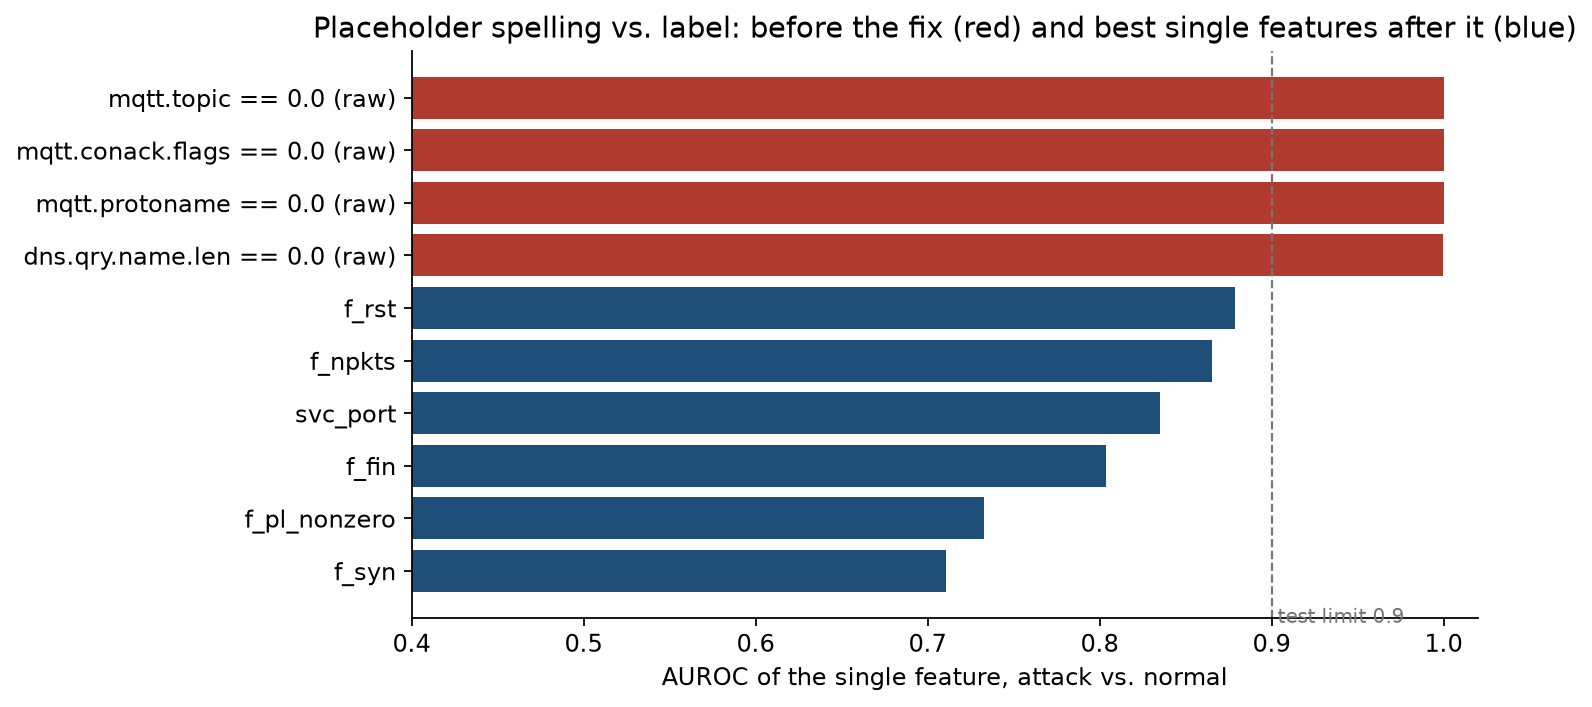
\includegraphics[width=0.8\linewidth]{figures/leak_auroc.png}
\caption{Single-feature AUROC before the placeholder fix (red) and best single features after it (blue)}
\label{fig:leakauroc}
\end{figure}
\begin{figure}[H]
\centering
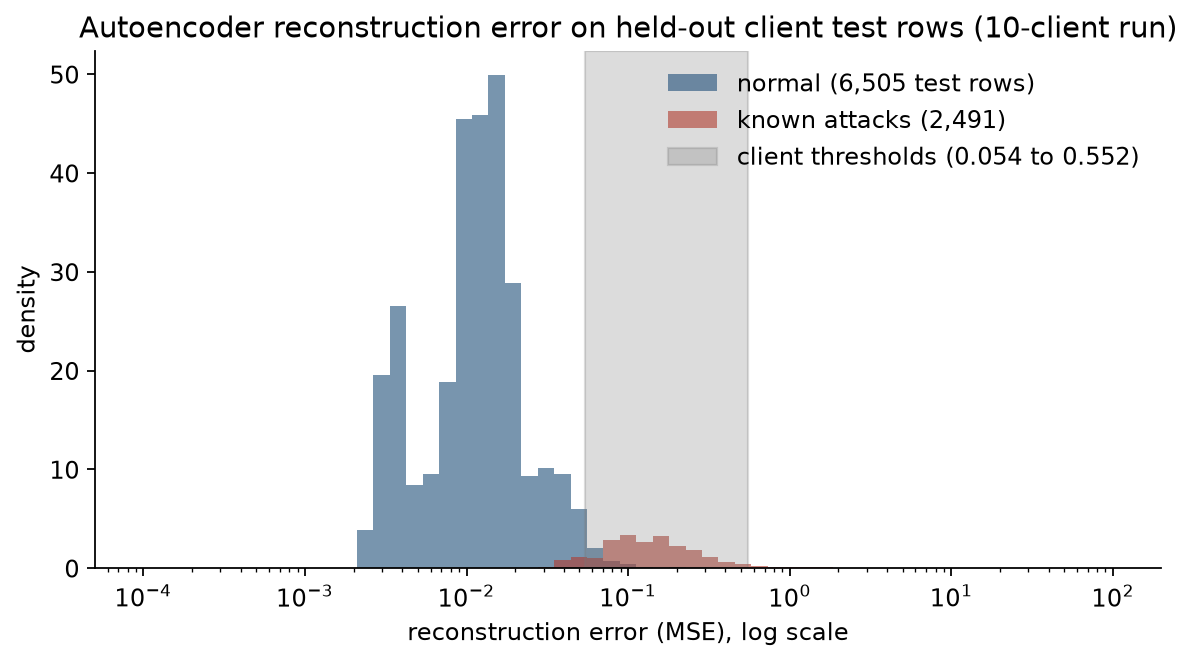
\includegraphics[width=0.8\linewidth]{figures/reconstruction_error.png}
\caption{Autoencoder reconstruction error on held-out client test rows (10-client run); grey band: range of the clients' thresholds}
\label{fig:reconerr}
\end{figure}
\begin{figure}[H]
\centering
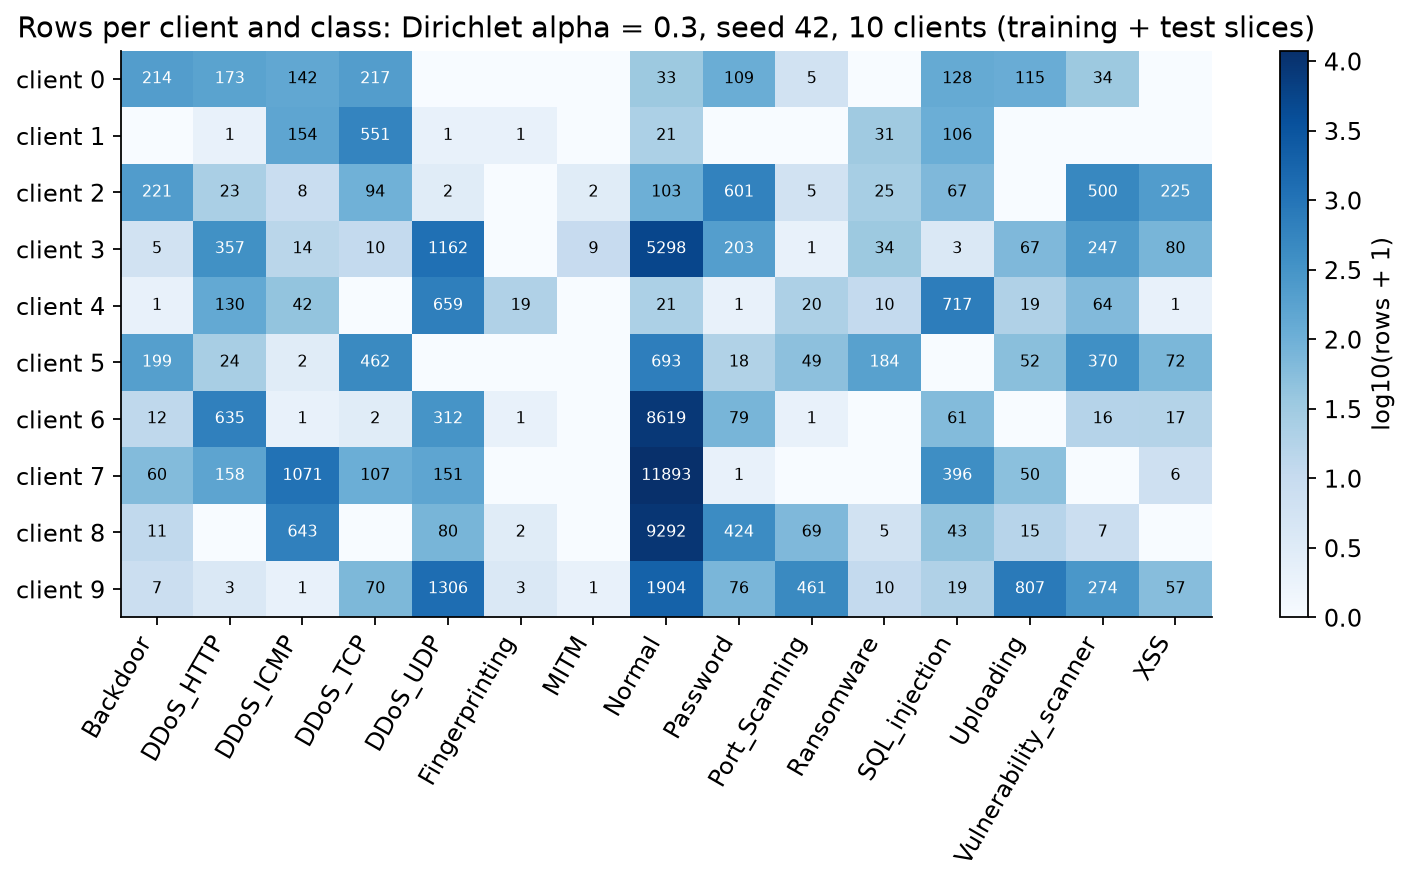
\includegraphics[width=0.98\linewidth]{figures/partition_heatmap.png}
\caption{Rows per client and class for the 10-client run (Dirichlet $\alpha=0.3$, seed 42)}
\label{fig:partheat}
\end{figure}
\begin{figure}[H]
\centering
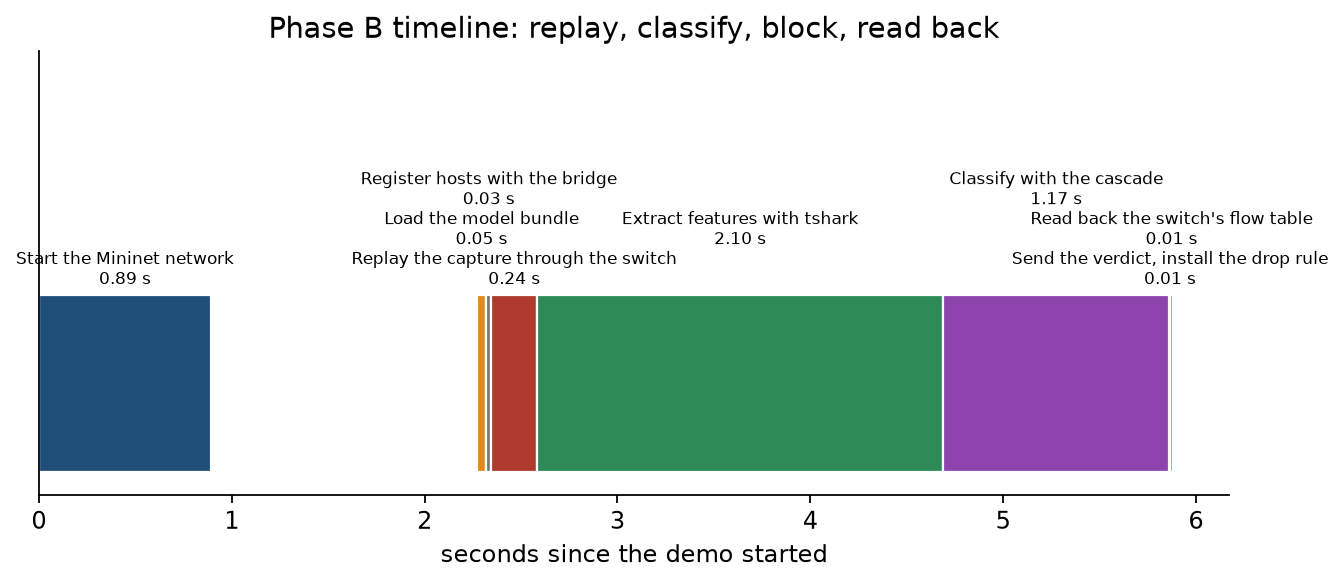
\includegraphics[width=0.9\linewidth]{figures/phase_b_timeline.png}
\caption{Phase B timeline for one replay of the Backdoor capture}
\label{fig:pbtimeline}
\end{figure}


\section{Limitations of the Study}\label{sec:limits}
\begin{enumerate}
  \item \textbf{One dataset, one testbed.} Every number comes from Edge-IIoTset. Its benign traffic is only MQTT and VNC, so the service-port feature is partly a testbed effect: in a network with benign web traffic the port alone would separate far less.
  \item \textbf{Mitigation is not inline.} Phase B classifies a capture after TShark has extracted features from all of it; for a replayed file nearly the whole capture had already passed through the default forwarding entry before the drop rule appeared. No per-packet blocking latency is measured or claimed, and the latency benchmark covers model time only (Section~\ref{sec:speed}).
  \item \textbf{Flow features describe whole flow records} (up to 120~s), so the classifier labels flow records rather than deciding on a first packet.
  \item \textbf{The trust filter is weaker at full scale.} Attacker survival at 30\% malicious clients is 0.50 to 0.62 on the whole dataset (0.12 to 0.27 on the 60{,}000-row pool); the cause is not established. The filter breaks down at 50\%, as median-based references do, and a white-box stealth attacker is mostly missed (survival 0.60 to 0.80 at full scale, 0.72 to 0.90 earlier). Only two attack models were tested.
  \item \textbf{The autoencoder backstop is weaker at full scale}: autoencoder-alone recall is 0.22 to 0.49 on the whole dataset. Clients that hold no benign validation rows (up to three of 20) get an infinite threshold, so their autoencoder never flags anything.
  \item \textbf{False alarms.} The 97th-percentile threshold gives about 3\% benign false alarms by construction. On the whole dataset 2.5\% to 16.3\% of normal packets are flagged, but only 0.34\% to 1.04\% of normal connections, because a few long normal connections dominate the packet count.
  \item \textbf{Small classes.} MITM is a single connection (406 rows) and cannot be split, so it is scored only by the zero-day experiment and the live replay; Fingerprinting has 872 rows. Per-class figures for these rest on very few test rows.
  \item \textbf{Zero-day detection depends on the class.} Uploading is the weakest held-out class (0.527 to 0.665), then MITM (0.751 to 1.000) and, depending on the seed, Backdoor and Vulnerability\_scanner.
  \item \textbf{Live replay.} The captures are the dataset's own, the released Vulnerability-scanner capture is damaged (its readable prefix was used), and two of the 14 captures are classified as the wrong attack type (both are still blocked).
  \item \textbf{Seeds.} The main experiments use three seeds, but the stealth-attacker, pruning and clipping tests at full scale use one, and no confidence intervals are given. Seed-to-seed variation is real (for example autoencoder-alone recall of 0.221 to 0.492 at 0 attackers).
  \item \textbf{Privacy relaxation.} The incremental classifier update sends at most 50 analyst-confirmed alert rows per surviving client to the server. The calibration set is also held centrally, so the classifier is not federated.
  \item \textbf{Pruning} reduces the model but clients still send dense updates, so no communication saving is demonstrated.
  \item \textbf{Emulation.} Clients are processes on one machine and the network is Mininet inside one virtual machine; there are no physical devices, hardware switch or network delays. Timings come from one machine and are upper bounds where other jobs shared it.
  \item \textbf{Comparability.} The dataset corrections (placeholder fix, MITM repair, connection split) mean the numbers cannot be compared directly with papers that train on the released CSV with a random split; the claim that those results are inflated is a reasoned expectation, not something this report measured on their pipelines.
  \item \textbf{Novelty} rests on targeted searches only, not a systematic literature review.
  \item \textbf{Deep-learning comparison.} The comparison of LightGBM with a neural classifier used a 500{,}000-row class-capped sample and a modest network, so only its relative result is meaningful.
\end{enumerate}

\section{Conclusion}
The results answer the four objectives as follows.
\begin{table}[H]
\centering
\small
\renewcommand{\arraystretch}{1.2}
\begin{tabular}{|>{\raggedright\arraybackslash}p{3.7cm}|>{\raggedright\arraybackslash}p{9.8cm}|}
\hline
\textbf{Objective} & \textbf{What the measurements show} \\ \hline
1. Malicious-client detection and filtering & Known-attack recall stays at 0.985 to 0.997 up to 50\% sign-flip clients on the whole dataset. At 30\% the filtered autoencoder keeps 0.245 to 0.490 recall alone, where plain FedAvg falls to 0.002 to 0.092. The filter lets more attackers through than at 60{,}000 rows and misses a stealth attacker. \\ \hline
2. Efficient, privacy-aware FL & Clients send only weights (9{,}834 parameters, about 39~kB) and error histograms; a 10-client run on 1.89 million rows takes 23 to 31 minutes and a 20-client run 18 to 21 minutes. Raw traffic stays on the client apart from the capped confirmed alerts. \\ \hline
3. Model optimisation (pruning) & Pruning during training costs autoencoder-alone recall (0.457 dense, 0.350 at 70\% sparsity, 0.198 at 90\%) while cascade macro-recall stays at 0.993 or above; no communication saving is shown because updates are still dense. \\ \hline
4. Semi-supervised, anomaly-based detection & On attack classes held out of all training, the cascade detects 0.895 to 0.944 on average, against 0.723 to 0.757 for the classifier alone and 0.590 to 0.728 for the autoencoder alone. \\ \hline
\end{tabular}
\caption{Objectives and the evidence for each (whole dataset, three seeds unless stated)}
\end{table}
Beyond the objectives, the stand-alone classifier reaches 99.72\% accuracy and 0.983 macro F1 on 397{,}073 test packets from connections it never saw, all 14 attack captures are blocked by a drop rule read back from the switch, and the models decide on a packet in a median 0.642~ms.

\chapter{Conclusion}\label{chap:conclusion}

\section*{Conclusion}
The five parts of FL-IDS work together on real IoT/IIoT traffic: a boosting classifier, a federated autoencoder backstop, a cosine-similarity trust filter, Flower-based federated learning, and SDN mitigation. Each part has a measured contribution, and the measurements were repeated on the whole Edge-IIoTset dataset, split by connection, rather than on a subsample split by row. All planned phases are complete.

\begin{itemize}
  \item \textbf{Accuracy target met.} With service-port, payload-content and flow features and square-root class weights, the LightGBM classifier reaches \textbf{99.7\% accuracy and 0.983--0.985 macro F1} when trained on 1.43 million packets and tested on 397 thousand packets from connections that never appear in training. That is up from 96.4\% and 0.889 with the original features. It holds across three seeds, and when the classifier is trained on only the 5\% server calibration set (99.7\% / 0.979).
  \item \textbf{The whole federated system works at full scale.} In six real multi-process runs (10 and 20 clients, three seeds, 1.89 million training rows) the cascade reaches 0.994--0.998 attack macro-recall. The trust-filtered autoencoder stays usable with up to 50\% sign-flip clients for known attacks, while plain FedAvg's autoencoder collapses.
  \item \textbf{The backstop pays off on unseen attacks.} When each attack class is held out of training in turn, the cascade detects 0.895--0.944 of the unseen class on average, against 0.723--0.757 for the classifier alone.
  \item \textbf{Detection drives enforcement.} All 14 attack captures replayed through Mininet end in a block decision and a drop rule read back from the switch; 12 of 14 are classified as the right attack type.
  \item \textbf{The models are fast; the pipeline is not inline.} A packet is decided in a median 0.642~ms (one thread), and a whole full-dataset training run takes 18 to 31 minutes. Mitigation is nonetheless capture-level, not per-packet.
  \item \textbf{Data quality.} The released Edge-IIoTset CSV contains a placeholder label leak (one feature with an AUROC of 1.0), first reported by Galal~\cite{galal2026provenance}, and column-shifted MITM rows, which we found and repaired. Results trained directly on it with a random split are likely inflated.
\end{itemize}
The limitations that qualify these results are listed in Section~\ref{sec:limits}.

\section*{Future Work}
\begin{enumerate}
  \item Make mitigation streaming: classify flows incrementally (for example after the first $n$ packets) so a rule can be installed while an attack is still running, and measure the end-to-end blocking latency.
  \item Defend against the white-box stealth attacker (Section~\ref{sec:followups}), which the filter mostly misses, for example with a small trusted root dataset as in FLTrust~\cite{cao2021fltrust}; measure zero-day detection under it; and test other adaptive strategies and attackers above 50\%.
  \item Find out why the trust filter excludes fewer attackers and the autoencoder is weaker at full scale, and repeat the stealth-attacker, pruning and clipping experiments at full scale over more seeds, with confidence intervals.
  \item Validate on a second dataset that contains benign web traffic, to measure how much the service-port feature depends on the testbed.
  \item Reduce the per-round communication as well: clients still send dense updates, so sparse updates and zero-day detection of pruned models remain to be tested.
  \item Federate the classifier itself (for example with histogram-based federated boosting) so the calibration set no longer needs to be held centrally.
  \item Deploy on physical edge hardware and a hardware OpenFlow switch, and measure real network delays.
\end{enumerate}


\clearpage
% ----- References -----
\renewcommand{\bibname}{REFERENCES} % report class titles thebibliography itself
\addcontentsline{toc}{chapter}{REFERENCES}
\begin{thebibliography}{99}
\bibitem{ferrag2022edge} M. A. Ferrag, O. Friha, D. Hamouda, L. Maglaras and H. Janicke, ``Edge-IIoTset: A New Comprehensive Realistic Cyber Security Dataset of IoT and IIoT Applications for Centralized and Federated Learning'', \textit{IEEE Access}, vol. 10, pp. 40281--40306, 2022, doi: 10.1109/ACCESS.2022.3165809.
\bibitem{mothukuri2022fl} V. Mothukuri, P. Khare, R. M. Parizi, S. Pouriyeh \textit{et al.}, ``Federated-Learning-Based Anomaly Detection for IoT Security Attacks'', \textit{IEEE Internet of Things Journal}, vol. 9, no. 4, 2022.
\bibitem{li2021deepfed} B. Li, Y. Wu, J. Song, R. Lu, T. Li and L. Zhao, ``DeepFed: Federated Deep Learning for Intrusion Detection in Industrial Cyber--Physical Systems'', \textit{IEEE Transactions on Industrial Informatics}, vol. 17, no. 8, Aug. 2021.
\bibitem{hernandez2025fliids} J. L. Hernandez-Ramos, G. Karopoulos, E. Chatzoglou, V. Kouliaridis, E. Marmol, A. Gonzalez-Vidal and G. Kambourakis, ``Intrusion Detection Based on Federated Learning: A Systematic Review'', \textit{ACM Computing Surveys}, vol. 57, no. 12, 2025, doi: 10.1145/3731596.
\bibitem{cao2021fltrust} X. Cao, M. Fang, J. Liu and N. Z. Gong, ``FLTrust: Byzantine-robust Federated Learning via Trust Bootstrapping'', in \textit{Proc. Network and Distributed System Security Symposium (NDSS)}, 2021.
\bibitem{xu2022signguard} J. Xu, S.-L. Huang, L. Song and T. Lan, ``Byzantine-robust Federated Learning through Collaborative Malicious Gradient Filtering'' (SignGuard), in \textit{Proc. IEEE International Conference on Distributed Computing Systems (ICDCS)}, 2022.
\bibitem{zhang2023lgbmae} H. Zhang, L. Ge, G. Zhang, J. Fan, D. Li and C. Xu, ``A two-stage intrusion detection method based on light gradient boosting machine and autoencoder'', \textit{Mathematical Biosciences and Engineering}, vol. 20, no. 4, 2023, doi: 10.3934/mbe.2023301.
\bibitem{elhouda2023mitfed} Z. Abou El Houda, A. S. Hafid and L. Khoukhi, ``MiTFed: A Privacy Preserving Collaborative Network Attack Mitigation Framework Based on Federated Learning Using SDN and Blockchain'', \textit{IEEE Transactions on Network Science and Engineering}, vol. 10, no. 4, pp. 1985--2001, 2023.
\bibitem{mcmahan2017fedavg} B. McMahan, E. Moore, D. Ramage, S. Hampson and B. A. y Arcas, ``Communication-Efficient Learning of Deep Networks from Decentralized Data'', in \textit{Proc. International Conference on Artificial Intelligence and Statistics (AISTATS)}, 2017.
\bibitem{yin2018trimmed} D. Yin, Y. Chen, K. Ramchandran and P. Bartlett, ``Byzantine-Robust Distributed Learning: Towards Optimal Statistical Rates'', in \textit{Proc. International Conference on Machine Learning (ICML)}, 2018.
\bibitem{ke2017lightgbm} G. Ke, Q. Meng, T. Finley, T. Wang, W. Chen, W. Ma, Q. Ye and T.-Y. Liu, ``LightGBM: A Highly Efficient Gradient Boosting Decision Tree'', in \textit{Advances in Neural Information Processing Systems (NeurIPS)}, 2017.
\bibitem{hsu2019noniid} T.-M. H. Hsu, H. Qi and M. Brown, ``Measuring the Effects of Non-Identical Data Distribution for Federated Visual Classification'', arXiv:1909.06335, 2019.
\bibitem{galal2026provenance} M. M. Galal, ``Provenance, Not Behaviour: A Serialisation Artifact in Edge-IIoTset and a Leakage-Free Benchmark for Precision-Agriculture Intrusion Detection'', arXiv:2608.15761 (preprint), Aug. 2026.
\bibitem{sharafaldin2018cicids} I. Sharafaldin, A. H. Lashkari and A. A. Ghorbani, ``Toward Generating a New Intrusion Detection Dataset and Intrusion Traffic Characterization'', in \textit{Proc. International Conference on Information Systems Security and Privacy (ICISSP)}, 2018.
\bibitem{kairouz2021} P. Kairouz \textit{et al.}, ``Advances and open problems in federated learning'', \textit{Found. Trends Mach. Learn.}, vol. 14, no. 1--2, pp. 1--210, 2021, doi: 10.1561/2200000083.
\bibitem{beutel2020} D. J. Beutel \textit{et al.}, ``Flower: A friendly federated learning research framework'', arXiv:2007.14390, 2020.
\bibitem{rey2022} V. Rey \textit{et al.}, ``Federated learning for malware detection in IoT devices'', \textit{Comput. Netw.}, vol. 204, art. no. 108693, 2022, doi: 10.1016/j.comnet.2021.108693.
\bibitem{nguyen2025fedmse} V. T. Nguyen and R. Beuran, ``FedMSE: Semi-supervised federated learning approach for IoT network intrusion detection'', \textit{Comput. Secur.}, vol. 151, art. no. 104337, 2025, doi: 10.1016/j.cose.2025.104337.
\bibitem{sazid2026} Z. Y. Sazid and R. Abbas, ``Cybersecurity in edge computing: A trust-aware federated hybrid intrusion detection framework'', arXiv:2609.39584 (preprint), 2026.
\bibitem{shahin2025} M. Shahin, A. Hosseinzadeh and F. Chen, ``A two-stage hybrid federated learning framework for privacy-preserving IoT anomaly detection and classification'', \textit{IoT}, vol. 6, no. 3, art. no. 48, 2025, doi: 10.3390/iot6030048.
\bibitem{pillai2026} N. Pillai and M. Mathivanan, ``FL-NDR: A federated unlearning-driven network detection and response system for DDoS defence in software-defined networks'', \textit{Int. J. Saf. Secur. Eng.}, vol. 16, no. 6, 2026, doi: 10.18280/ijsse.160615.
\bibitem{blanchard2017} P. Blanchard \textit{et al.}, ``Machine learning with adversaries: Byzantine tolerant gradient descent'', in \textit{Advances in Neural Information Processing Systems 30}, 2017.
\bibitem{fang2020} M. Fang \textit{et al.}, ``Local model poisoning attacks to Byzantine-robust federated learning'', in \textit{Proc. 29th USENIX Secur. Symp.}, pp. 1623--1640, 2020.
\bibitem{li2021spatial} Z. Li \textit{et al.}, ``Byzantine-robust federated learning through spatial-temporal analysis of local model updates'', in \textit{Proc. IEEE 27th Int. Conf. Parallel Distrib. Syst. (ICPADS)}, pp. 372--379, 2021, doi: 10.1109/ICPADS53394.2021.00052.
\bibitem{fung2020} C. Fung, C. J. M. Yoon and I. Beschastnikh, ``The limitations of federated learning in sybil settings'', in \textit{Proc. 23rd Int. Symp. Res. Attacks, Intrusions Defenses (RAID)}, pp. 301--316, 2020.
\bibitem{zhu2024cosine} T. Zhu \textit{et al.}, ``Byzantine-robust federated learning via cosine similarity aggregation'', \textit{Comput. Netw.}, vol. 254, art. no. 110730, 2024, doi: 10.1016/j.comnet.2024.110730.
\bibitem{li2024experimental} S. Li, E. C. Ngai and T. Voigt, ``An experimental study of Byzantine-robust aggregation schemes in federated learning'', \textit{IEEE Trans. Big Data}, vol. 10, no. 6, pp. 975--988, 2024, doi: 10.1109/TBDATA.2023.3237397.
\bibitem{thein2024} T. T. Thein, Y. Shiraishi and M. Morii, ``Personalized federated learning-based intrusion detection system: Poisoning attack and defense'', \textit{Future Gener. Comput. Syst.}, vol. 153, pp. 182--192, 2024, doi: 10.1016/j.future.2023.10.005.
\bibitem{luong2024} T. Luong \textit{et al.}, ``Fed-LSAE: Thwarting poisoning attacks against federated cyber threat detection system via autoencoder-based latent space inspection'', \textit{J. Inf. Secur. Appl.}, vol. 87, art. no. 103916, 2024, doi: 10.1016/j.jisa.2024.103916.
\bibitem{mirsky2018} Y. Mirsky \textit{et al.}, ``Kitsune: An ensemble of autoencoders for online network intrusion detection'', in \textit{Proc. Netw. Distrib. Syst. Secur. Symp. (NDSS)}, 2018, doi: 10.14722/ndss.2018.23204.
\bibitem{engelen2021} G. Engelen, V. Rimmer and W. Joosen, ``Troubleshooting an intrusion detection dataset: The CICIDS2017 case study'', in \textit{Proc. IEEE Secur. Privacy Workshops (SPW)}, pp. 7--12, 2021, doi: 10.1109/SPW53761.2021.00009.
\bibitem{vaccari2020} I. Vaccari \textit{et al.}, ``MQTTset, a new dataset for machine learning techniques on MQTT'', \textit{Sensors}, vol. 20, no. 22, art. no. 6578, 2020, doi: 10.3390/s20226578.
\bibitem{firouzi2025} A. Firouzi \textit{et al.}, ``DataSense: A real-time sensor-based benchmark dataset for attack analysis in IIoT with multi-objective feature selection'', \textit{Electronics}, vol. 14, no. 20, art. no. 4095, 2025, doi: 10.3390/electronics14204095.
\bibitem{sommer2010} R. Sommer and V. Paxson, ``Outside the closed world: On using machine learning for network intrusion detection'', in \textit{Proc. IEEE Symp. Secur. Privacy}, pp. 305--316, 2010, doi: 10.1109/SP.2010.25.
\bibitem{arp2022} D. Arp \textit{et al.}, ``Dos and don'ts of machine learning in computer security'', in \textit{Proc. 31st USENIX Secur. Symp.}, pp. 3971--3988, 2022.
\bibitem{mckeown2008} N. McKeown \textit{et al.}, ``OpenFlow: Enabling innovation in campus networks'', \textit{ACM SIGCOMM Comput. Commun. Rev.}, vol. 38, no. 2, pp. 69--74, 2008, doi: 10.1145/1355734.1355746.
\bibitem{lantz2010} B. Lantz, B. Heller and N. McKeown, ``A network in a laptop: Rapid prototyping for software-defined networks'', in \textit{Proc. 9th ACM SIGCOMM Workshop Hot Topics Netw. (HotNets)}, pp. 1--6, 2010, doi: 10.1145/1868447.1868466.
\bibitem{chen2016xgboost} T. Chen and C. Guestrin, ``XGBoost: A scalable tree boosting system'', in \textit{Proc. 22nd ACM SIGKDD Int. Conf. Knowl. Discovery Data Mining}, pp. 785--794, 2016, doi: 10.1145/2939672.2939785.
\end{thebibliography}
\clearpage
\chapter*{Plagiarism}
\addcontentsline{toc}{chapter}{PLAGIARISM}
The similarity check and the AI-generated-content check of this report were run with the DrillBit software (submission ID 7421657, 4 November 2026) on the 90-page version of the report. The similarity index is 4\% and the AI-generated text detected is 1.06\%. The two report pages follow.
\clearpage
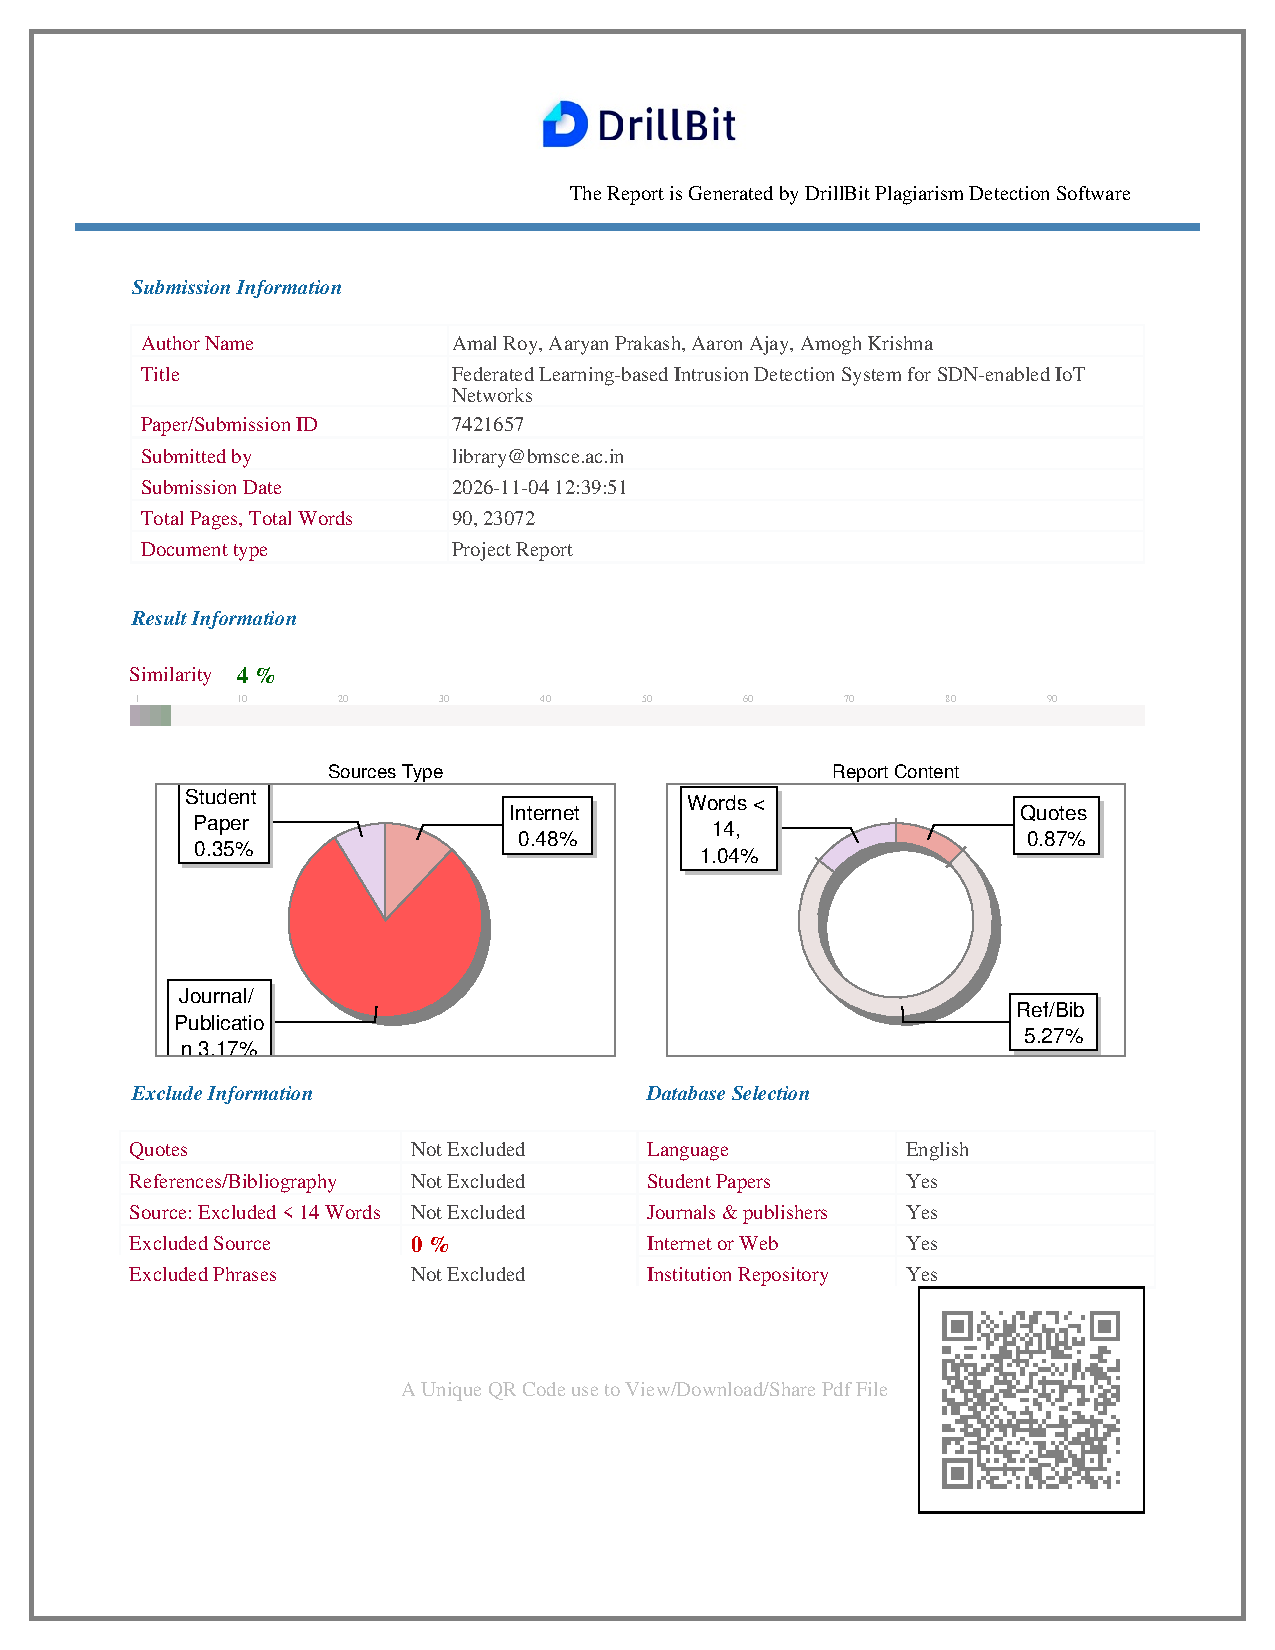
\includepdf[pages=1,scale=0.92,pagecommand={\thispagestyle{empty}}]{similarity_report.pdf}
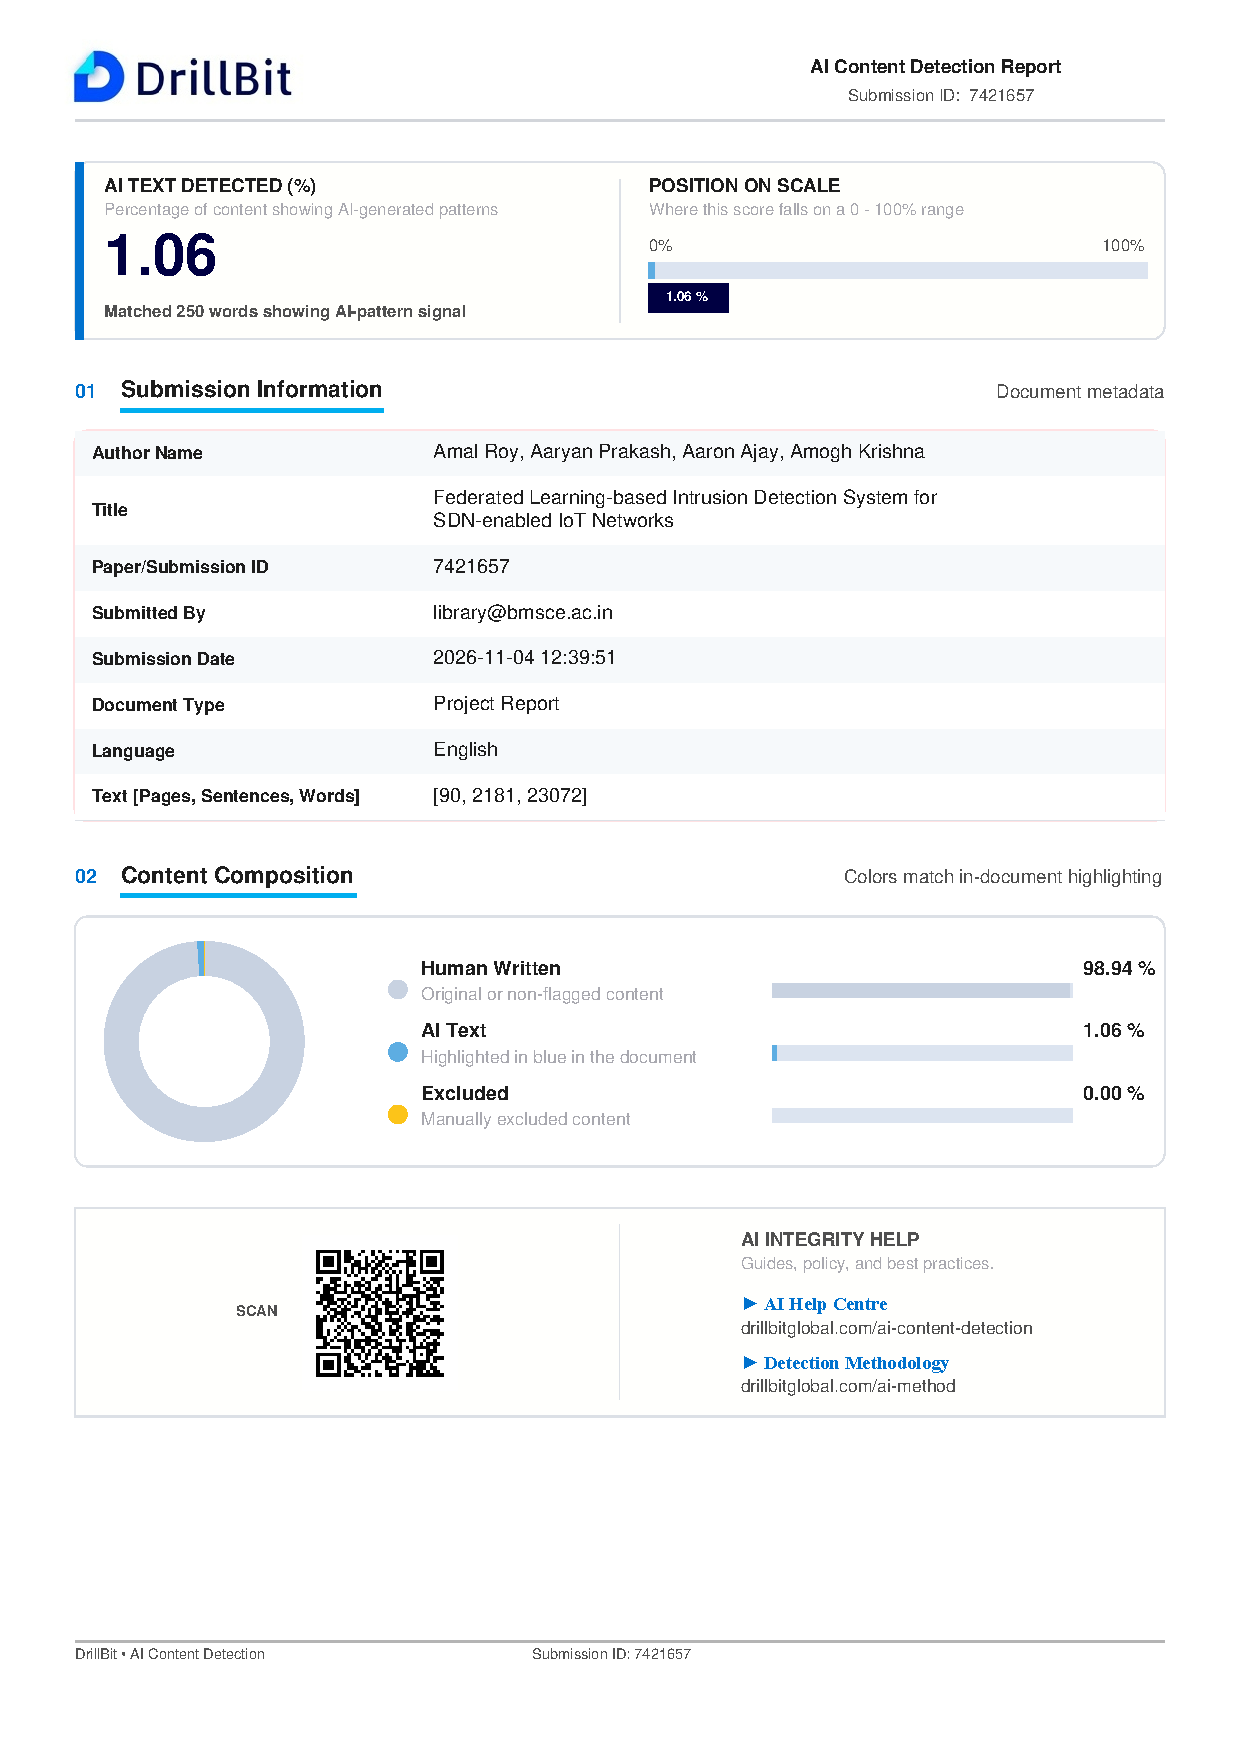
\includepdf[pages=1,scale=0.92,pagecommand={\thispagestyle{empty}}]{ai_report_p1.pdf}

% ----- Appendices -----
\appendix
\renewcommand{\thechapter}{\Alph{chapter}}
\renewcommand{\thesection}{\Roman{section}}
\section {Appendix A: Snapshots}
\begin{figure}[H]
\centering
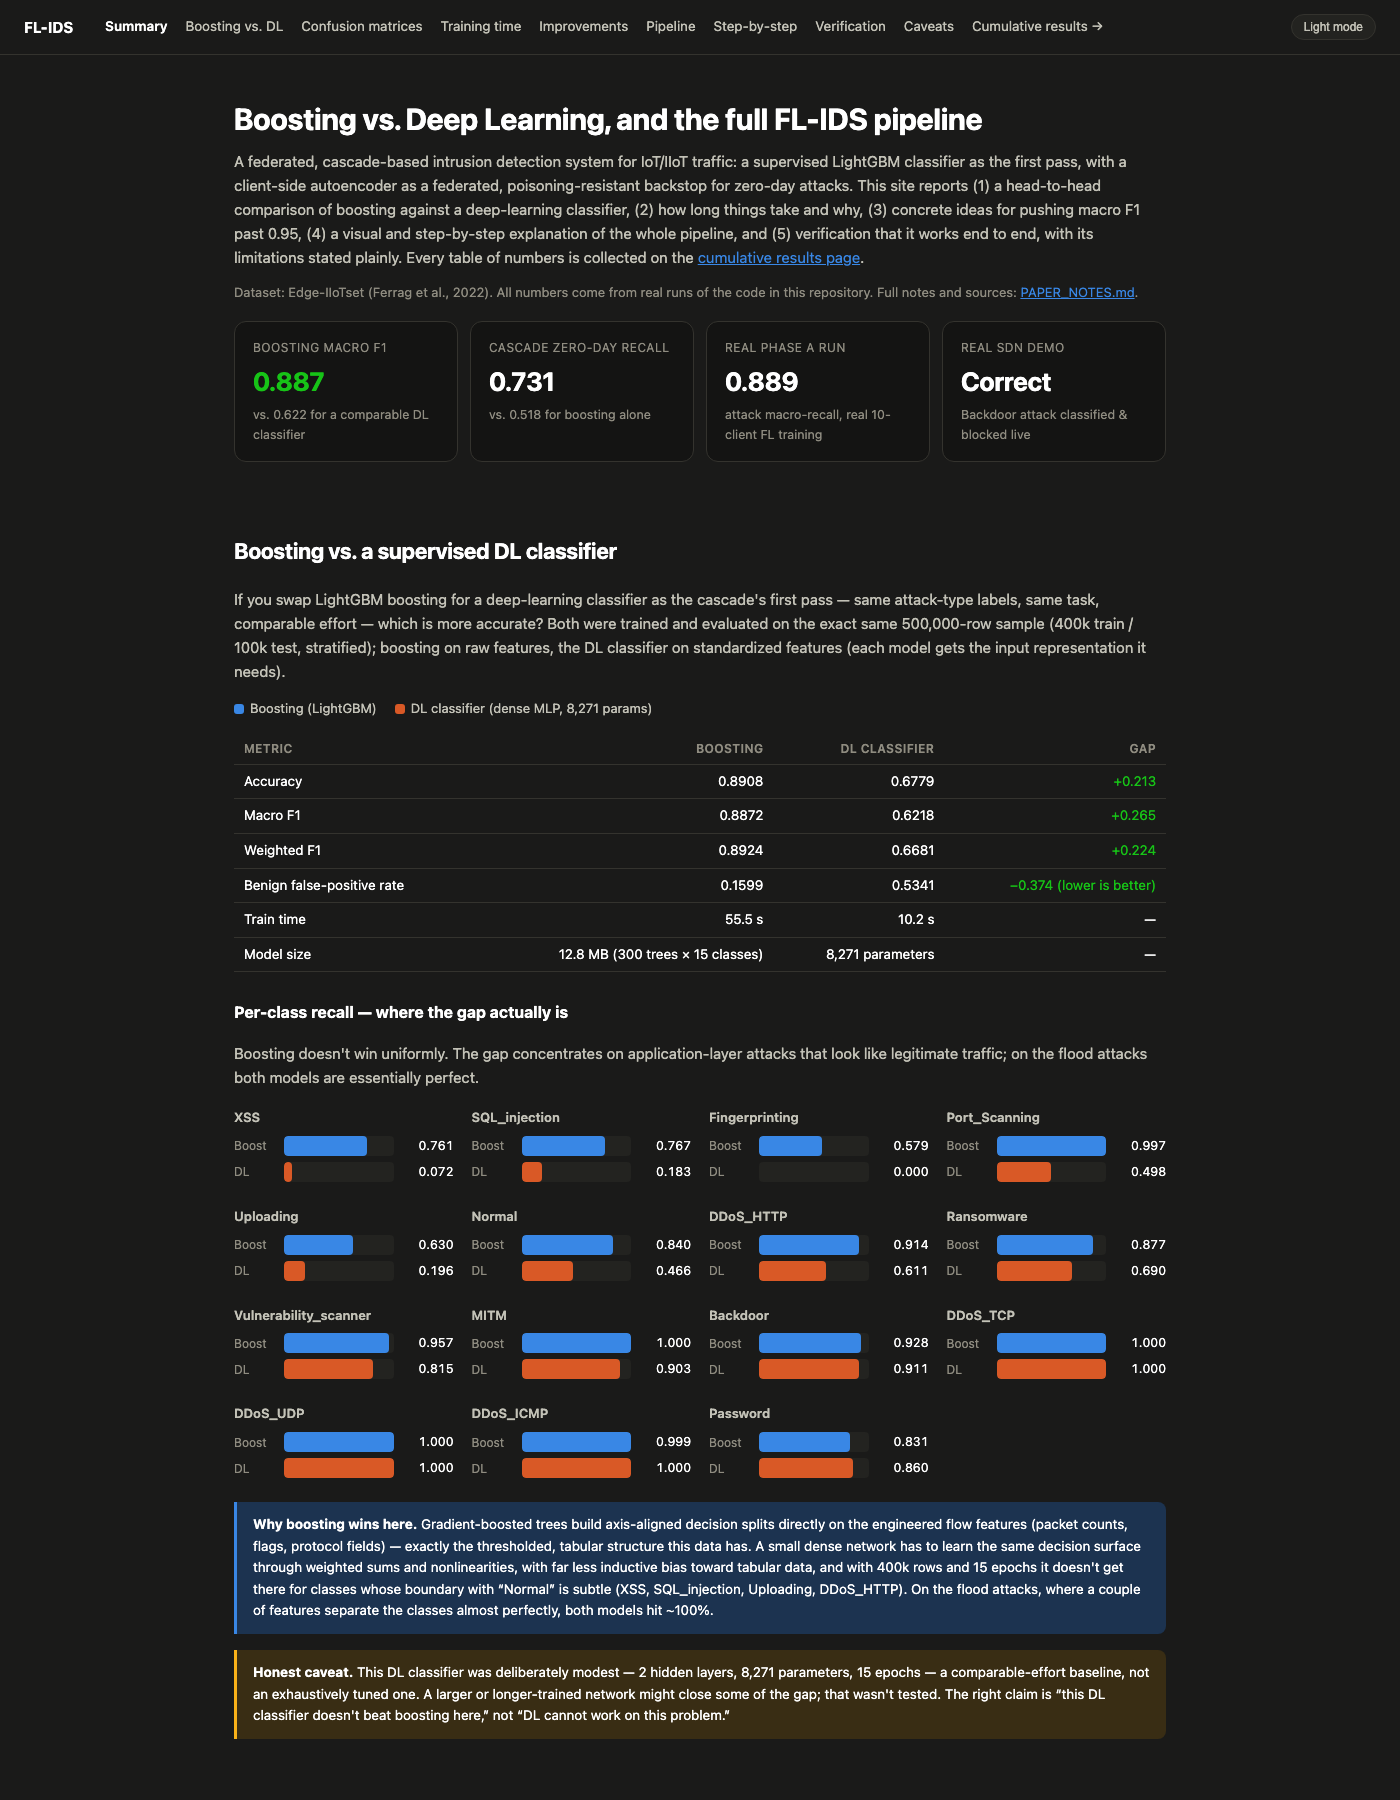
\includegraphics[width=0.9\linewidth]{figures/website.png}
\caption{Project results website (\url{https://theaaryanprakash.github.io/FL-IDS-SDN/results/}). A second, presentation-style site with animated diagrams is at \url{https://theaaryanprakash.github.io/FL-IDS-SDN/}}
\end{figure}
\noindent\textbf{Phase B result} (\texttt{runs/phase\_b/phase\_b\_result.json}, excerpt):
\begin{verbatim}
"classification": "Backdoor", "confidence": 0.9974,
"stage": "boosting", "num_packets": 24914,
"num_non_benign": 23895
"mitigation": {"action": "block", "applied": true,
               "ip_address": "10.0.0.1"}
flow table:
 priority=100,ip,nw_src=10.0.0.1 actions=drop
 priority=0 actions=NORMAL   (n_packets=23586)
"check": {"action": "block", "consistent": true}
\end{verbatim}
\noindent\textbf{Automated test suite:}
\begin{verbatim}
244 passed, 1 skipped, 2 warnings in 462.87s (0:07:42)
\end{verbatim}

\subsection*{Snapshots of the live arena: changing the network}
The arena (\url{https://theaaryanprakash.github.io/FL-IDS-SDN/arena/}) lets a user edit the topology and then press Play. Every verdict shown is the real output of the cascade for that client's model and capture; the packets themselves are not sent in the hosted version. Figures~\ref{fig:snap:sample}--\ref{fig:snap:normal} show what happens when the network changes.

\begin{figure}[H]
\centering
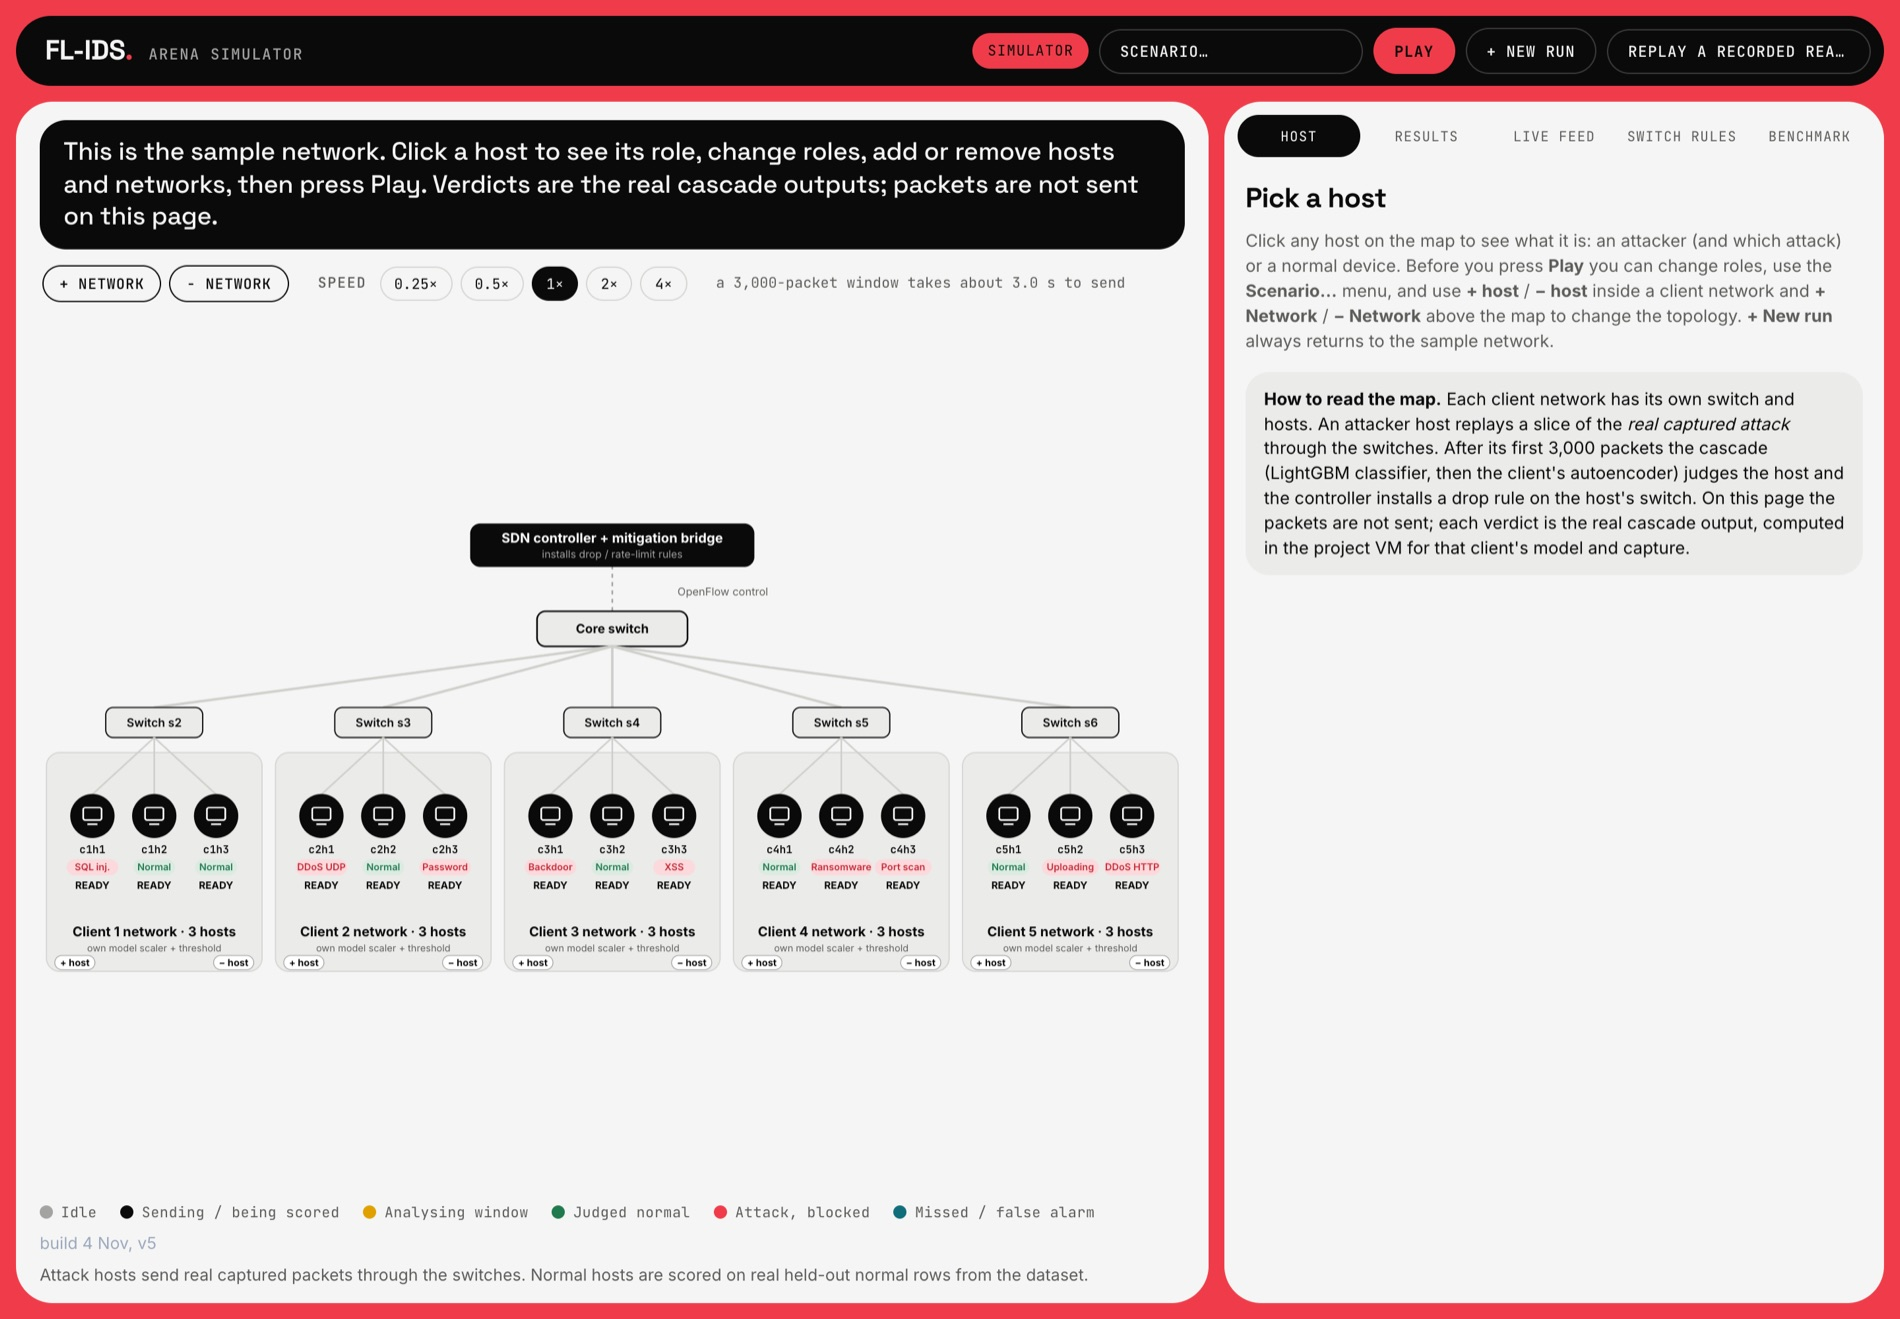
\includegraphics[width=0.84\linewidth]{figures/snap_arena_sample.jpg}
\caption{The arena at start: the sample network of five client networks with three hosts each, a core switch and the SDN controller. Attack hosts carry a named attack, the others are normal.}
\label{fig:snap:sample}
\end{figure}

\begin{figure}[H]
\centering
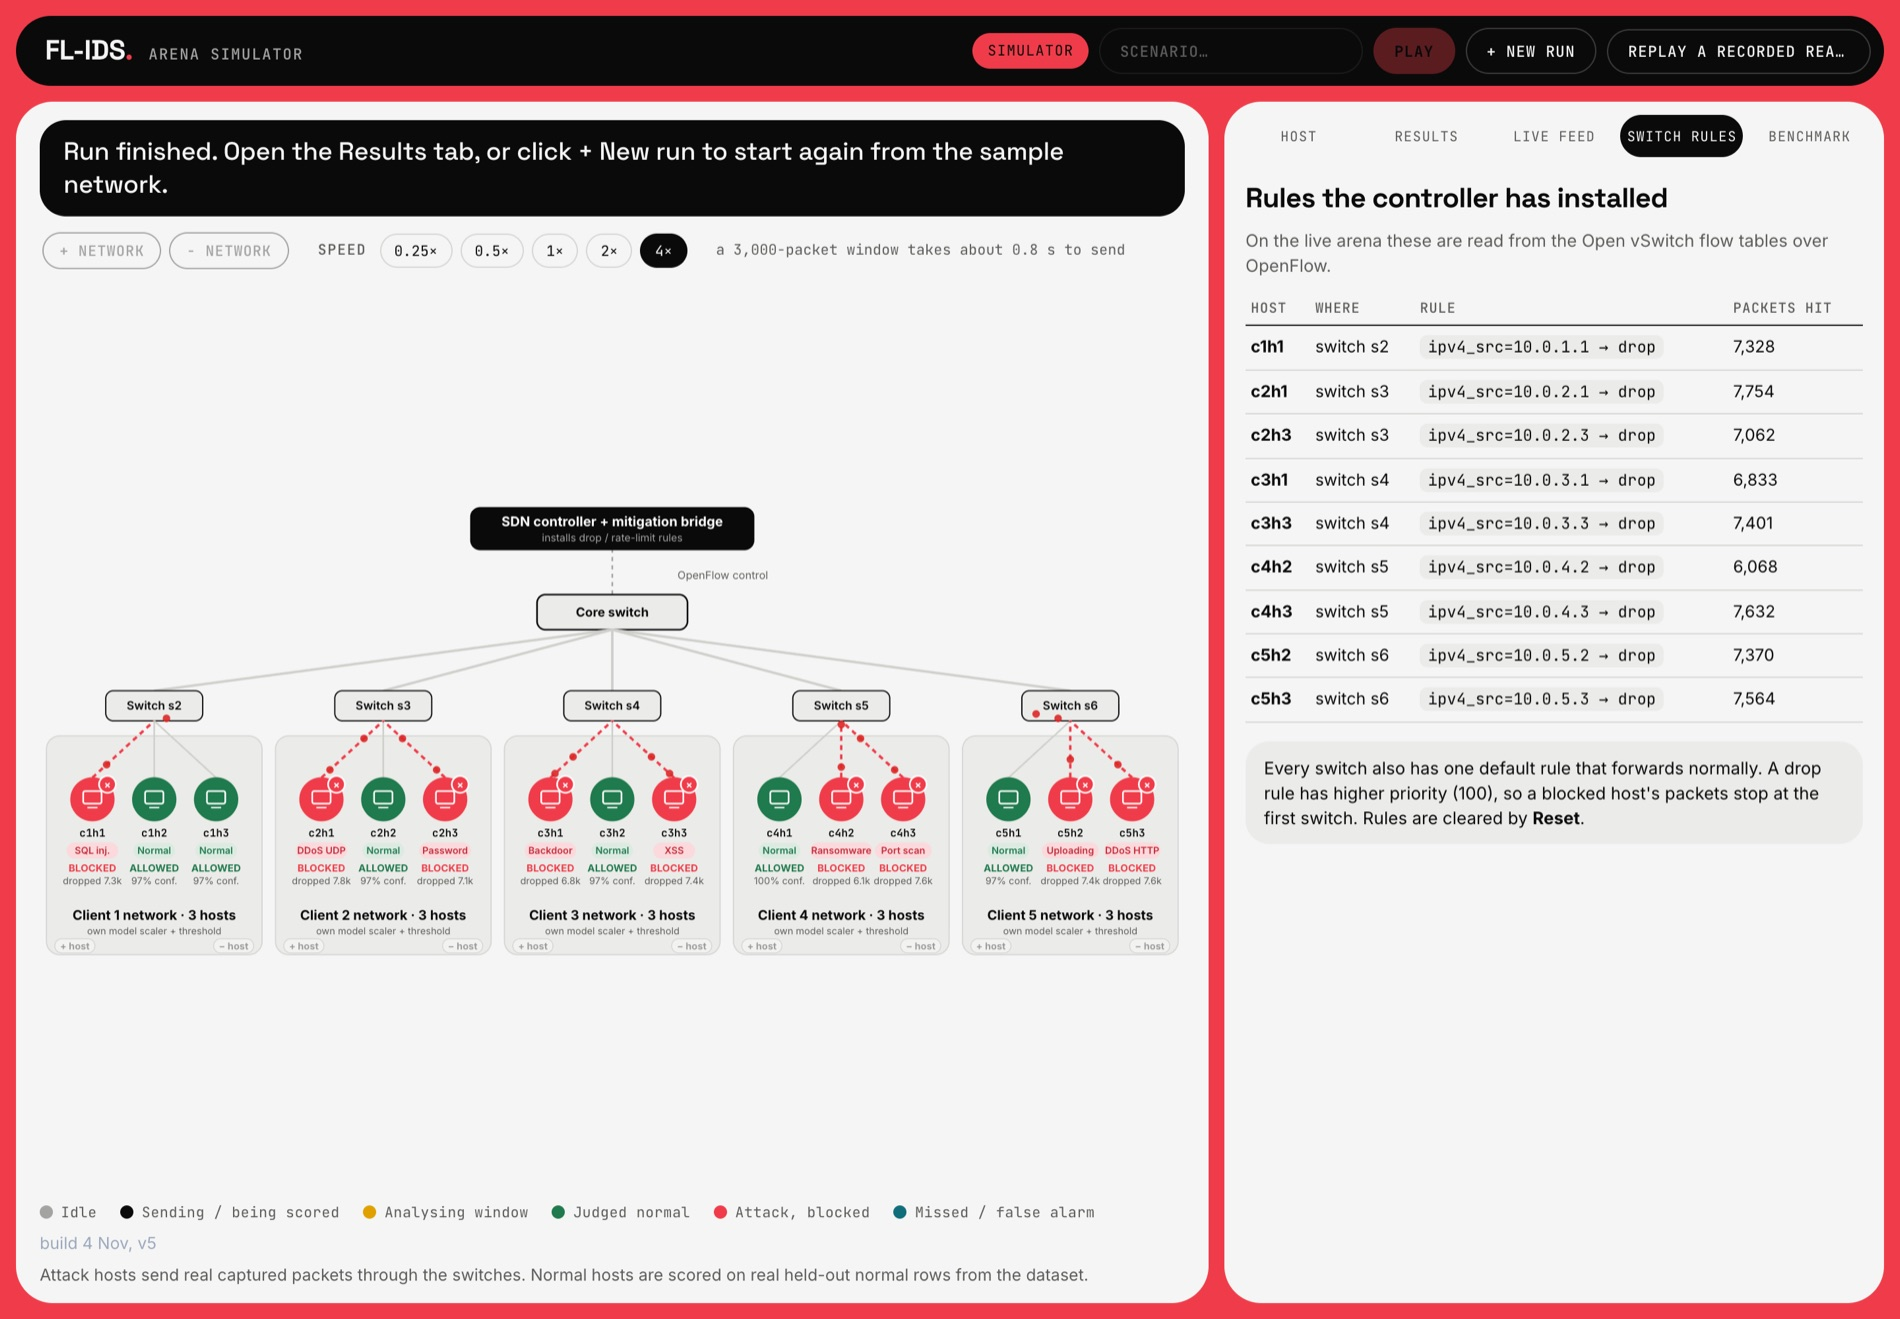
\includegraphics[width=0.84\linewidth]{figures/snap_arena_rules.jpg}
\caption{Run on the sample network, Switch rules tab. The controller installed nine \texttt{ipv4\_src=\ldots $\rightarrow$ drop} rules, one on the first switch of each attacking host, with 6,068 to 7,754 packets dropped by each rule. The six normal hosts have no rule.}
\label{fig:snap:rules}
\end{figure}

\begin{figure}[H]
\centering
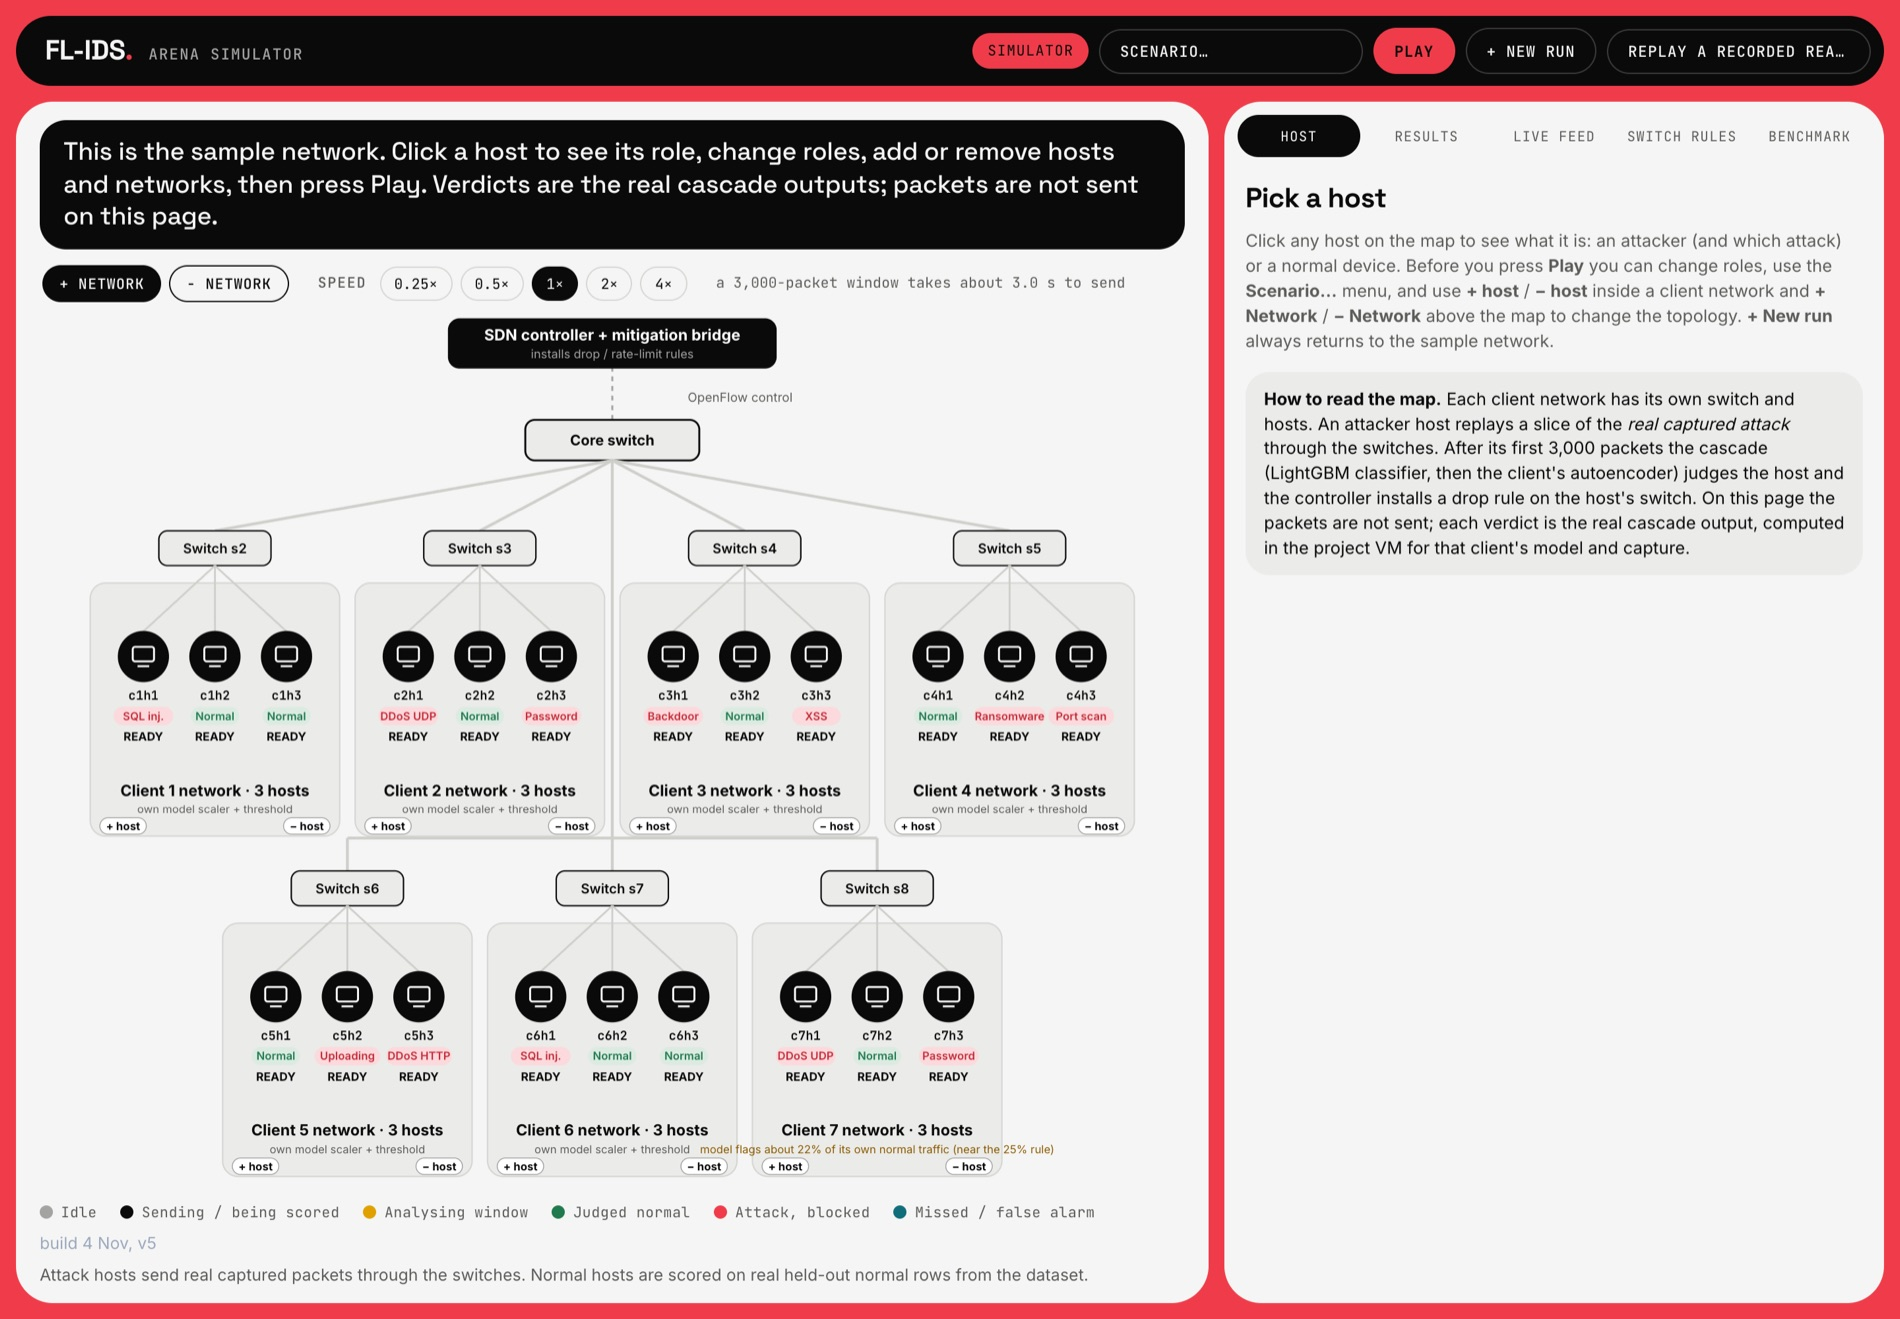
\includegraphics[width=0.84\linewidth]{figures/snap_arena_added_ready.jpg}
\caption{\textbf{Adding networks.} Two networks were added with \emph{+ Network}: Client~6 and Client~7, with their own switches s7 and s8, give seven client networks in all. The Mixed scenario was then applied, so every host has a role and is ready to run.}
\label{fig:snap:addready}
\end{figure}

\begin{figure}[H]
\centering
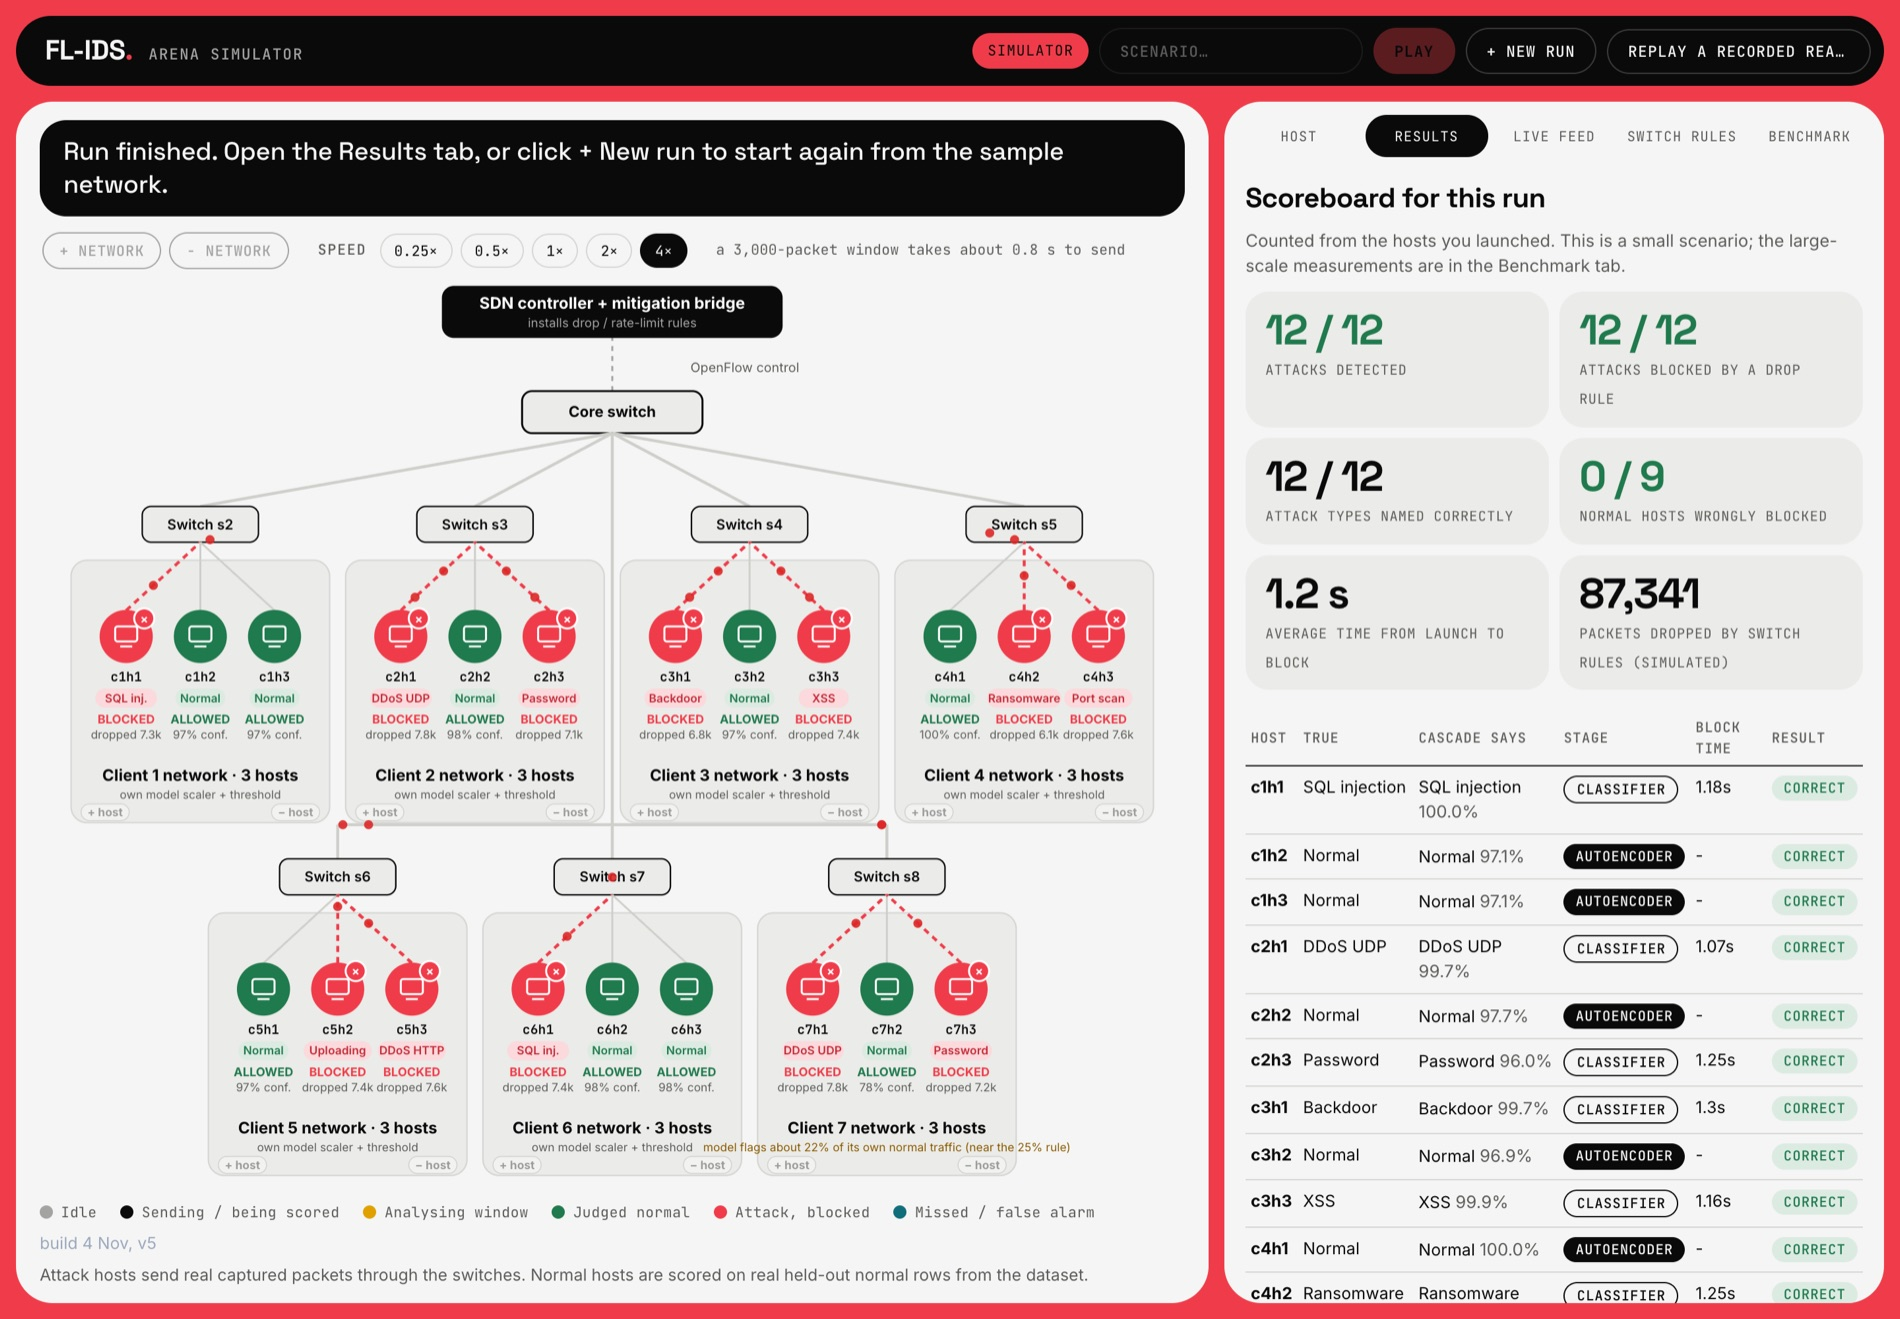
\includegraphics[width=0.84\linewidth]{figures/snap_arena_added_results.jpg}
\caption{After adding two networks and pressing Play: 12 of 12 attacks detected, blocked by a drop rule and named correctly, and 0 of 9 normal hosts blocked. The average time from launch to block was 1.2~s and the switch rules dropped 87,341 packets. The arena warns that the model of Client~7 flags about 22\% of its own normal traffic, close to the 25\% limit of the alarm rule.}
\label{fig:snap:addresults}
\end{figure}

\begin{figure}[H]
\centering
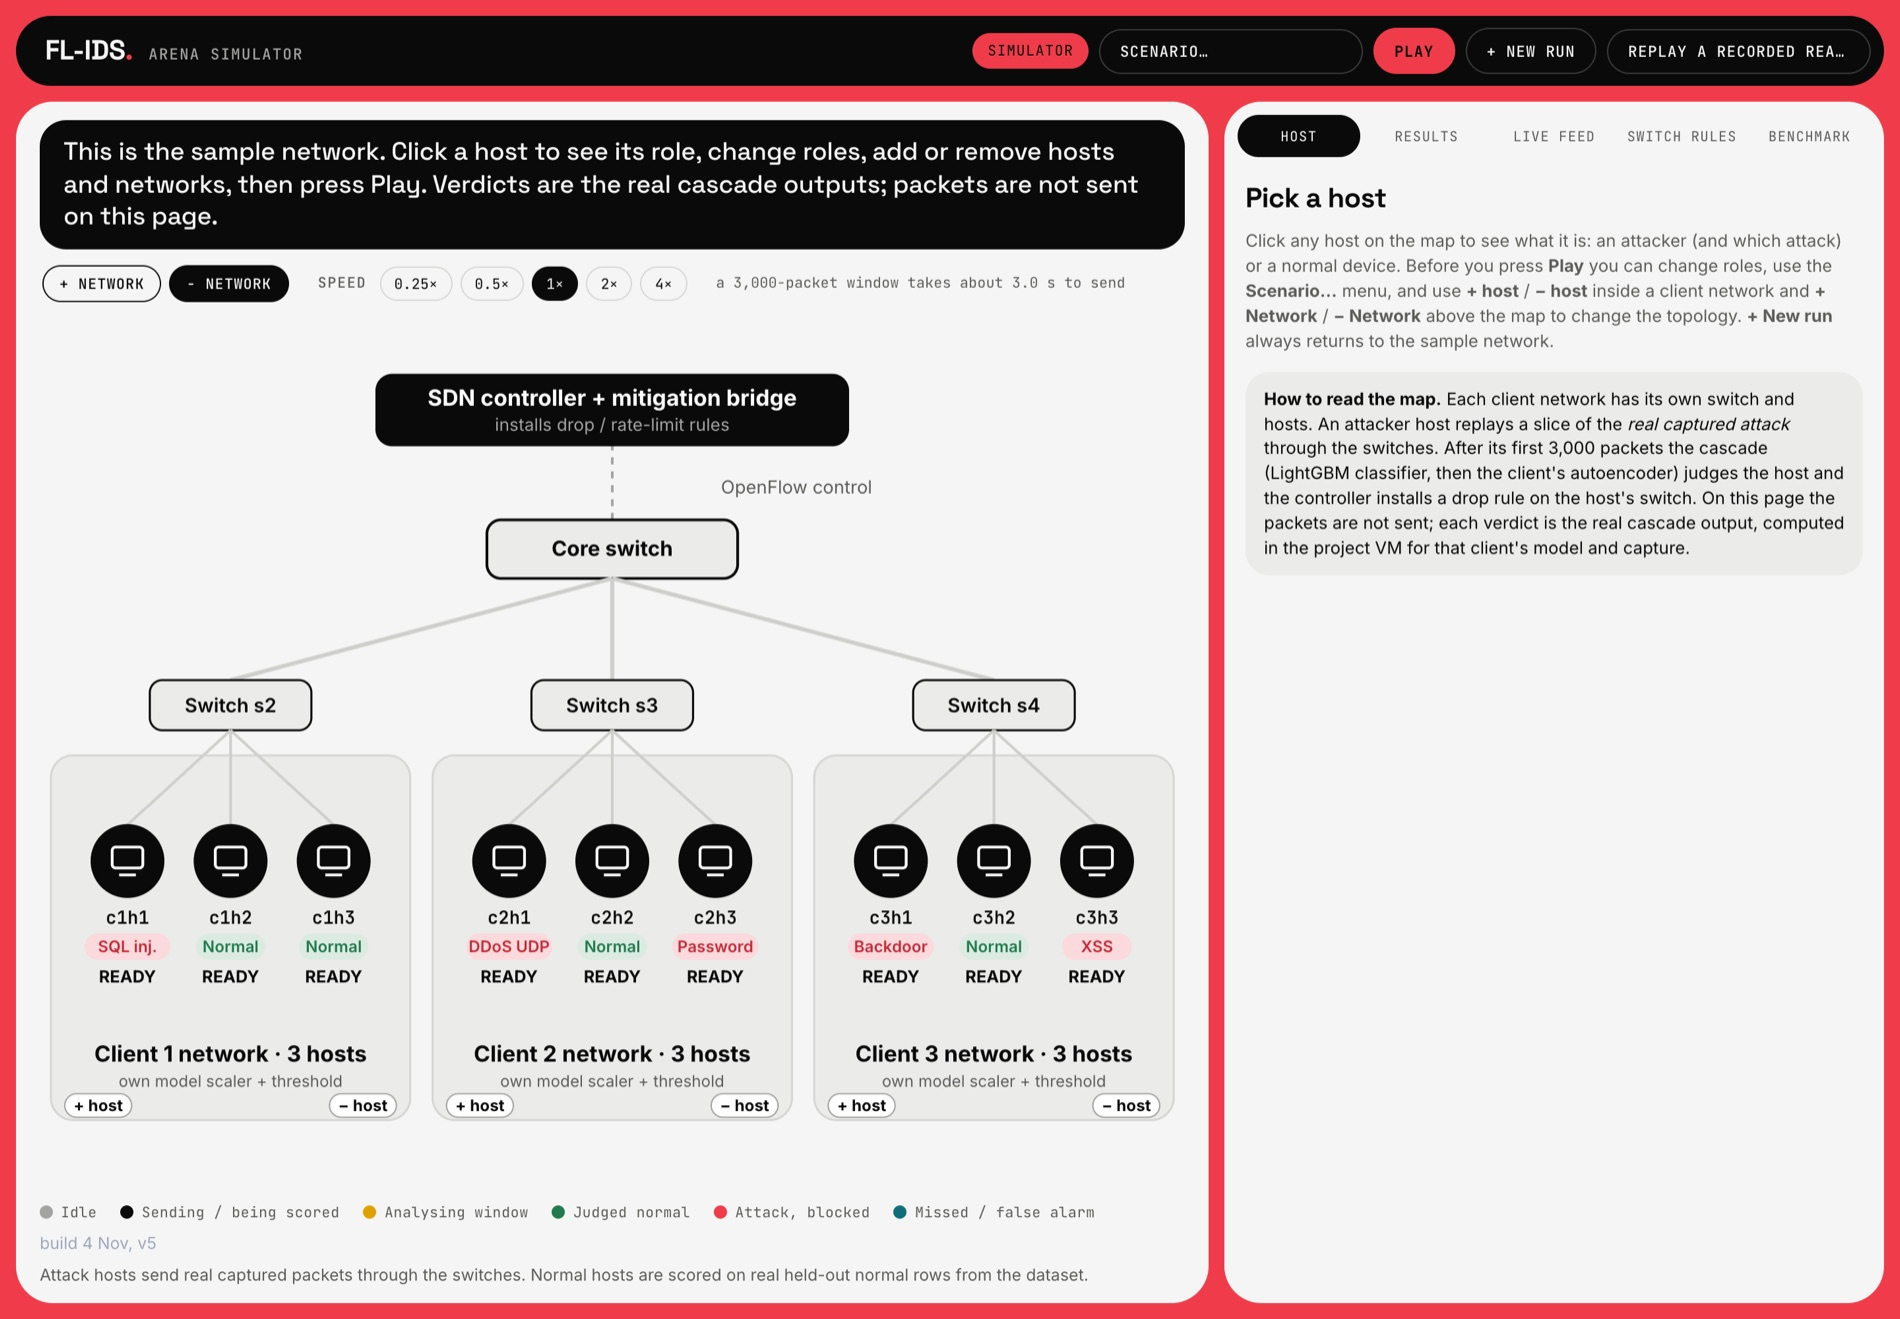
\includegraphics[width=0.84\linewidth]{figures/snap_arena_removed_ready.jpg}
\caption{\textbf{Removing networks.} Two networks were removed with \emph{-- Network}, leaving three client networks under the core switch. The Mixed scenario was applied to the remaining hosts. The controller and the remaining switches are unchanged.}
\label{fig:snap:rmready}
\end{figure}

\begin{figure}[H]
\centering
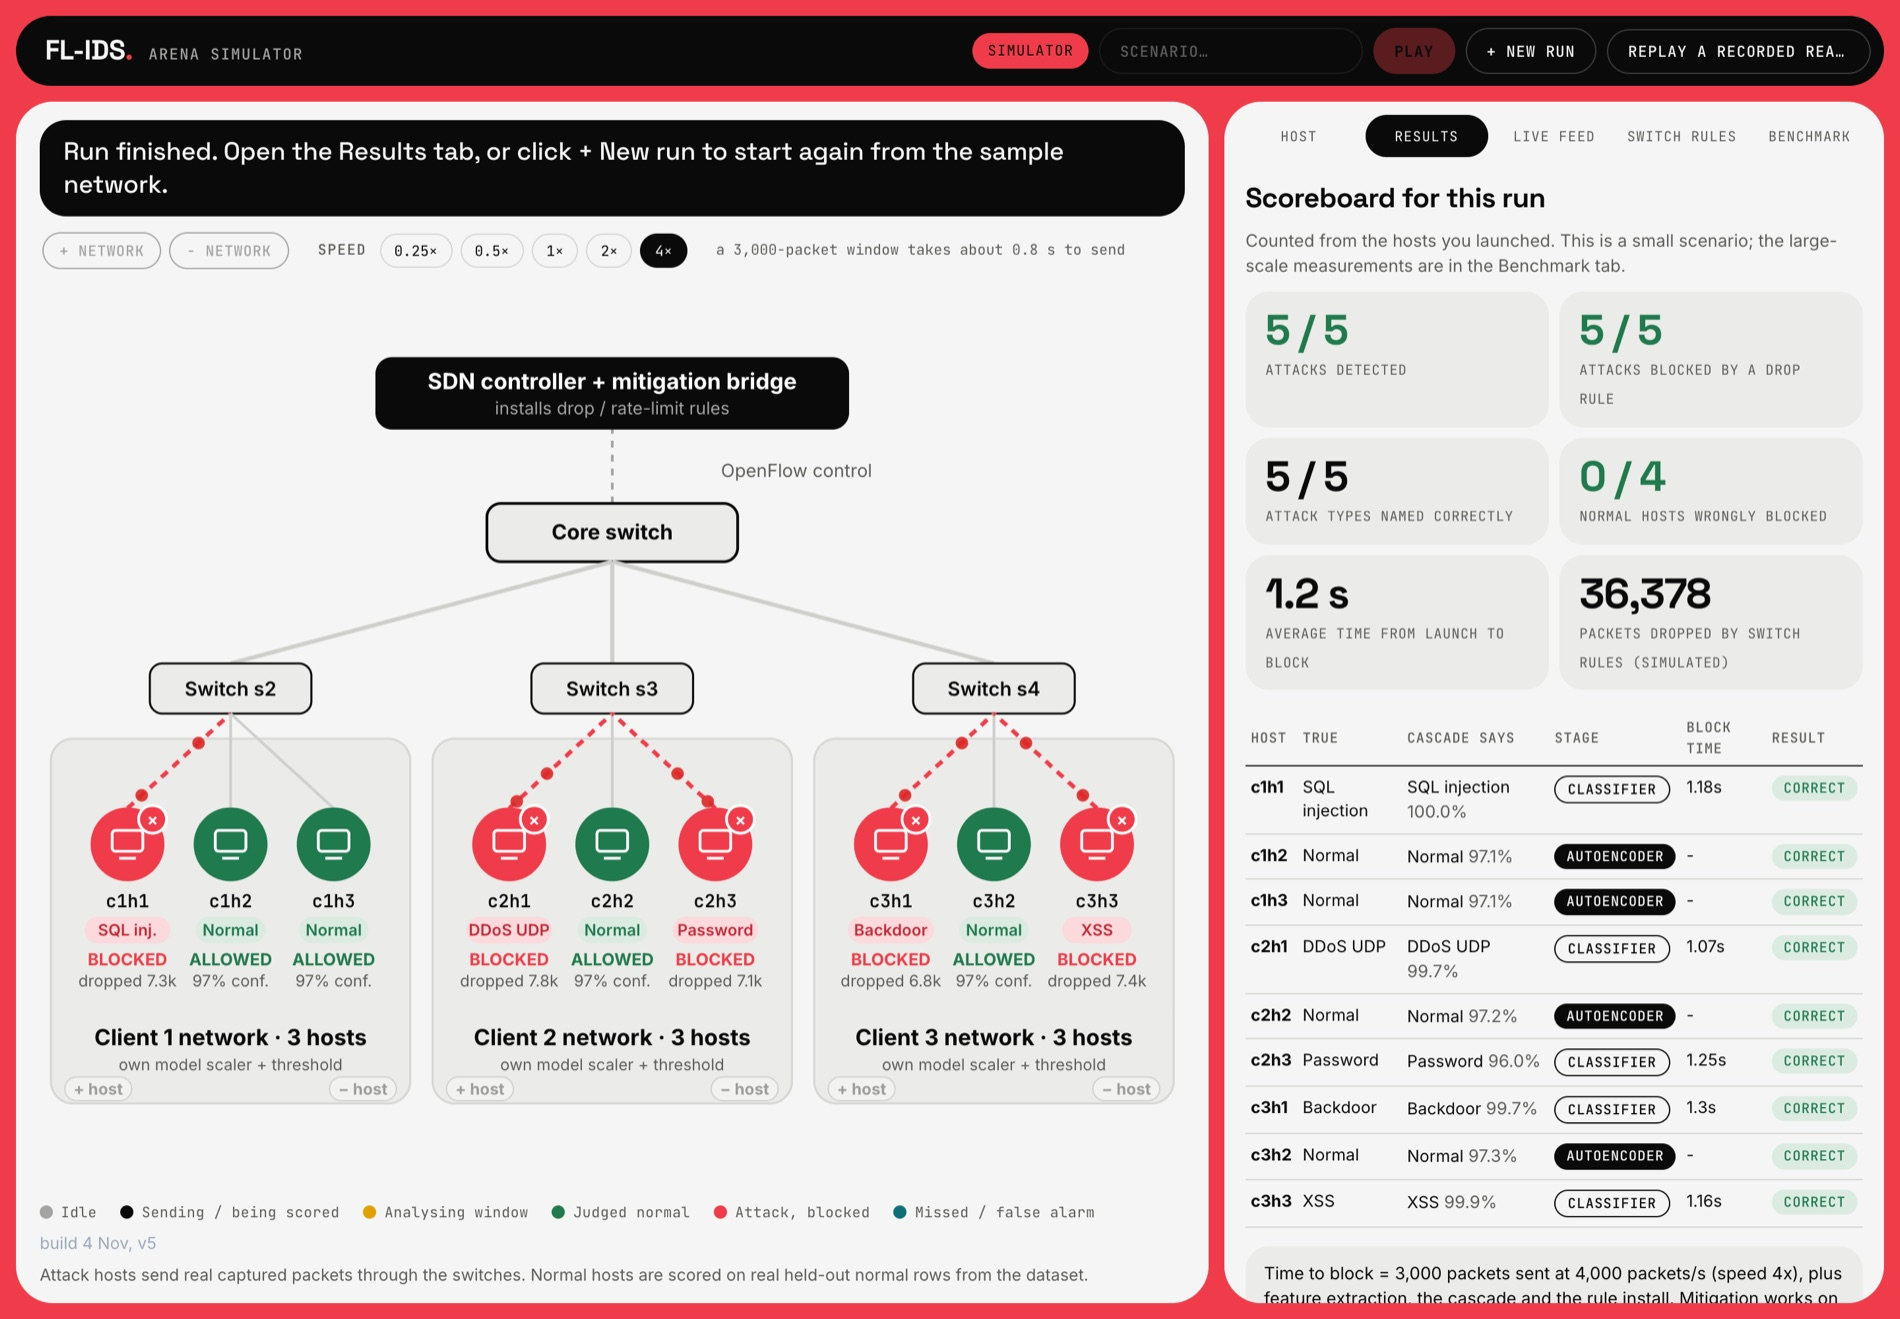
\includegraphics[width=0.84\linewidth]{figures/snap_arena_removed_results.jpg}
\caption{After removing two networks and pressing Play: 5 of 5 attacks detected, blocked and named correctly, 0 of 4 normal hosts blocked, 36,378 packets dropped. A smaller network behaves exactly like the larger one, because every client decides with its own model and threshold.}
\label{fig:snap:rmresults}
\end{figure}

\begin{figure}[H]
\centering
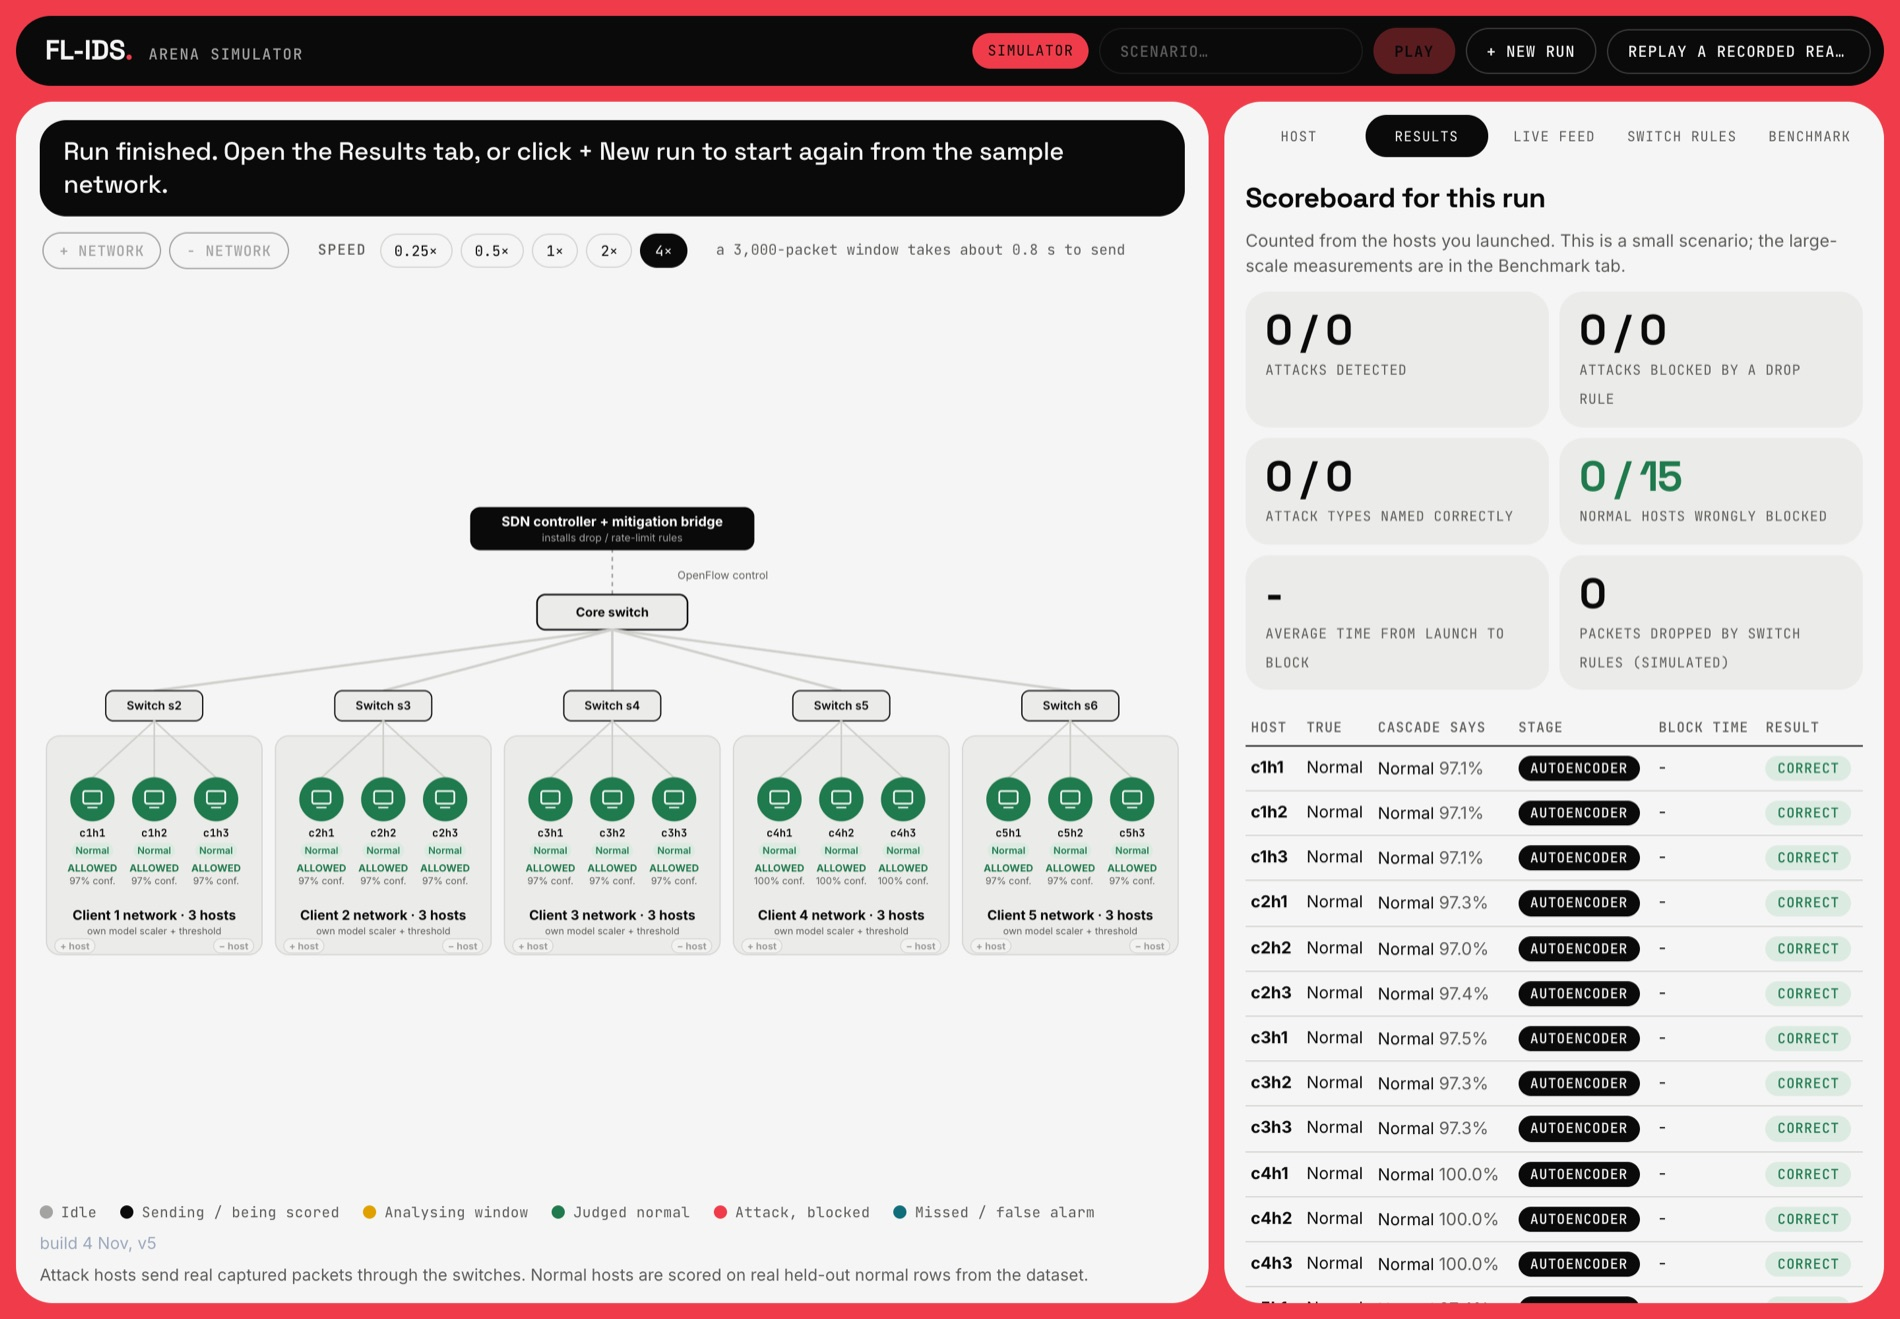
\includegraphics[width=0.84\linewidth]{figures/snap_arena_normal.jpg}
\caption{False-alarm check: every host is set to normal. All 15 hosts are judged normal by the autoencoder stage with 97 to 100\% confidence, no rule is installed (0 of 15 normal hosts wrongly blocked) and no packet is dropped.}
\label{fig:snap:normal}
\end{figure}

\begin{figure}[H]
\centering
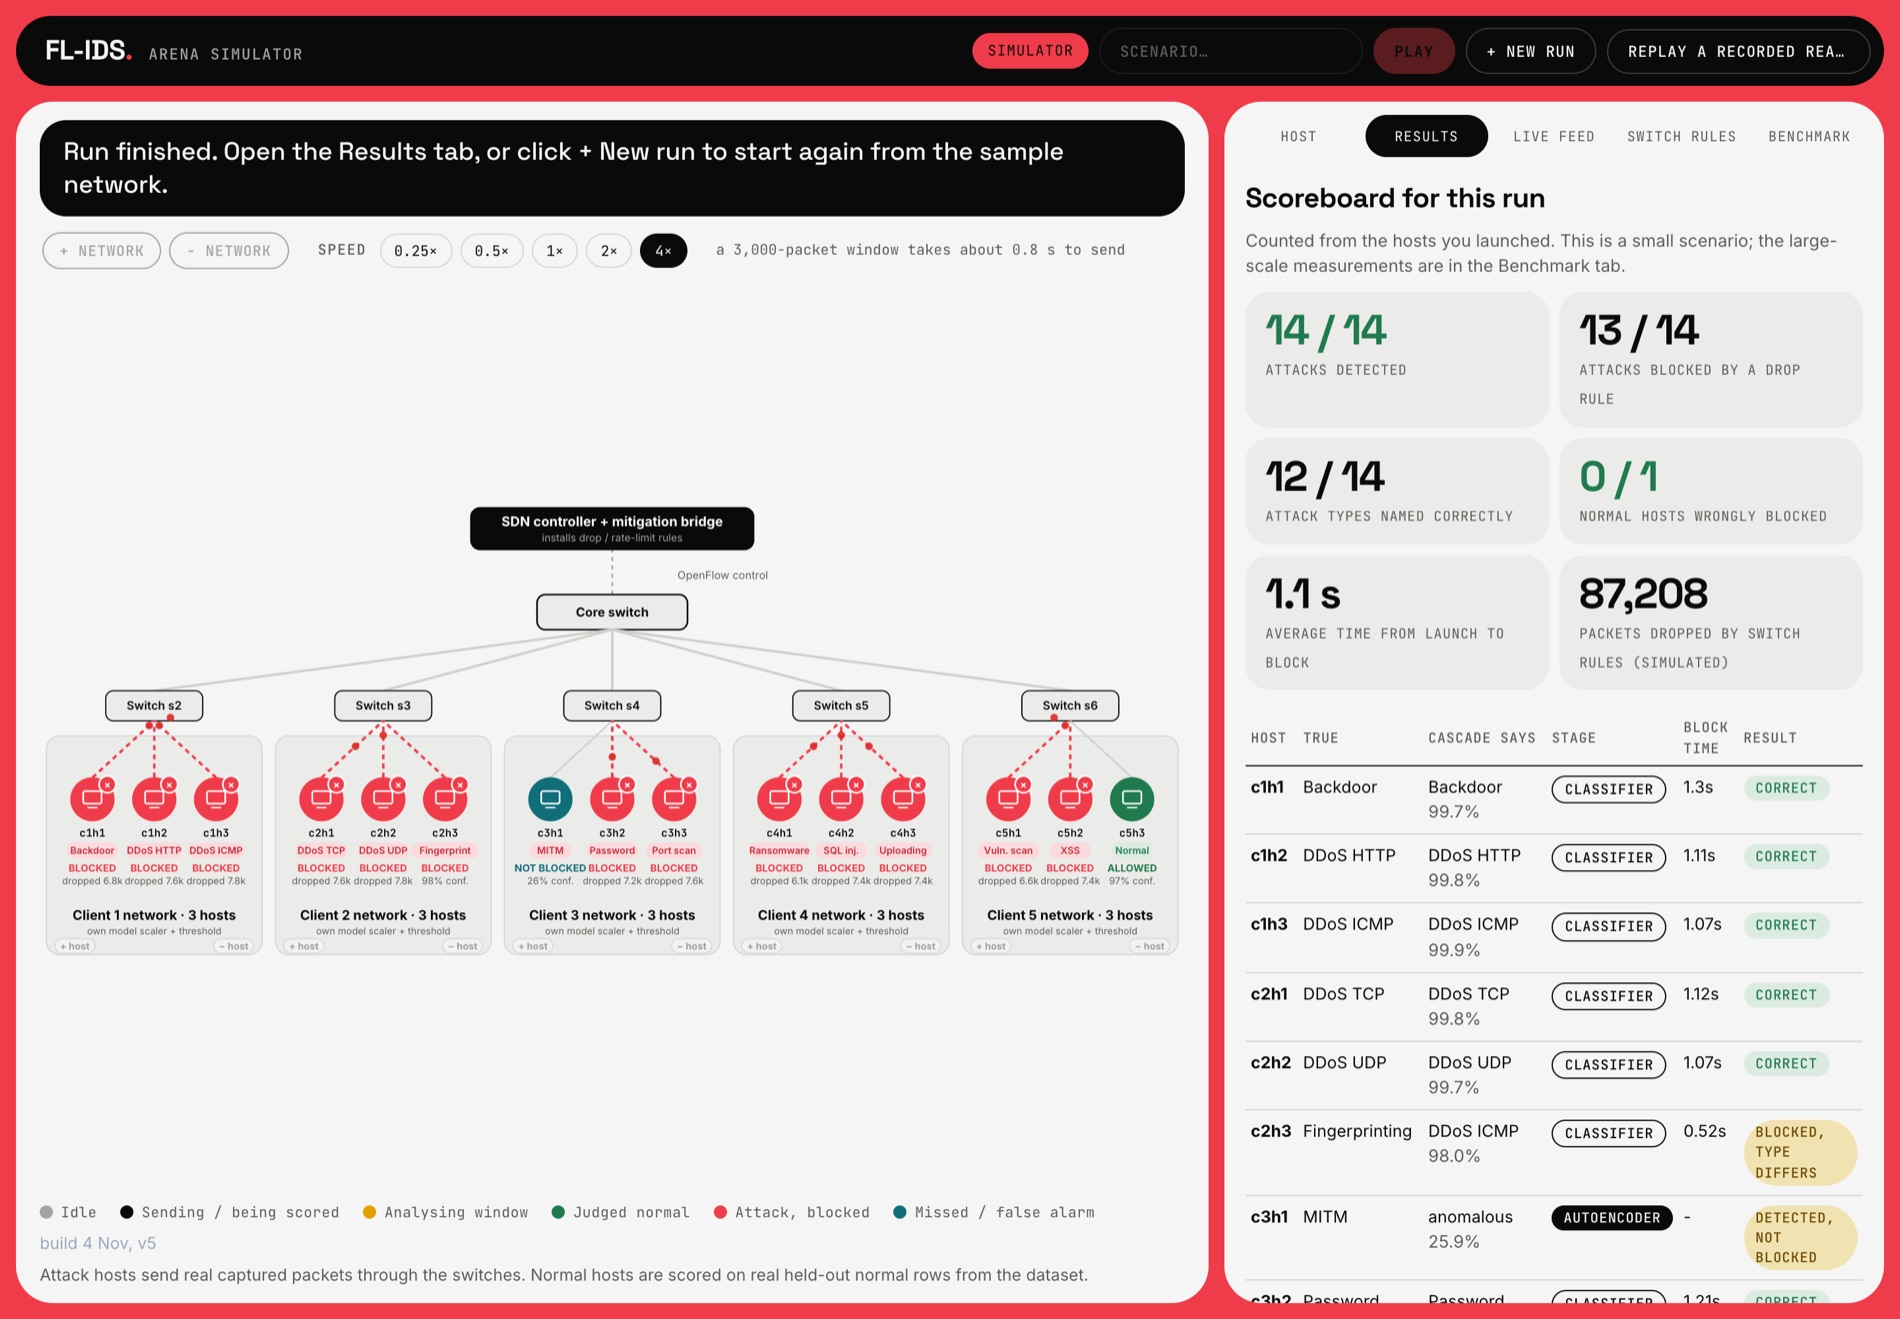
\includegraphics[width=0.84\linewidth]{figures/snap_arena_all14.jpg}
\caption{All 14 attack types at once (one normal host). The scoreboard shows 14 of 14 attacks detected, 13 of 14 blocked by a drop rule, 12 of 14 named correctly and 0 of 1 normal hosts blocked, with 87,208 packets dropped. Two cases are not perfect, and the arena marks them: Fingerprinting is blocked but named as DDoS ICMP, and the MITM host is detected by the autoencoder at only 26\% confidence, below the blocking threshold, so it is detected but not blocked.}
\label{fig:snap:all14}
\end{figure}

\begin{figure}[H]
\centering
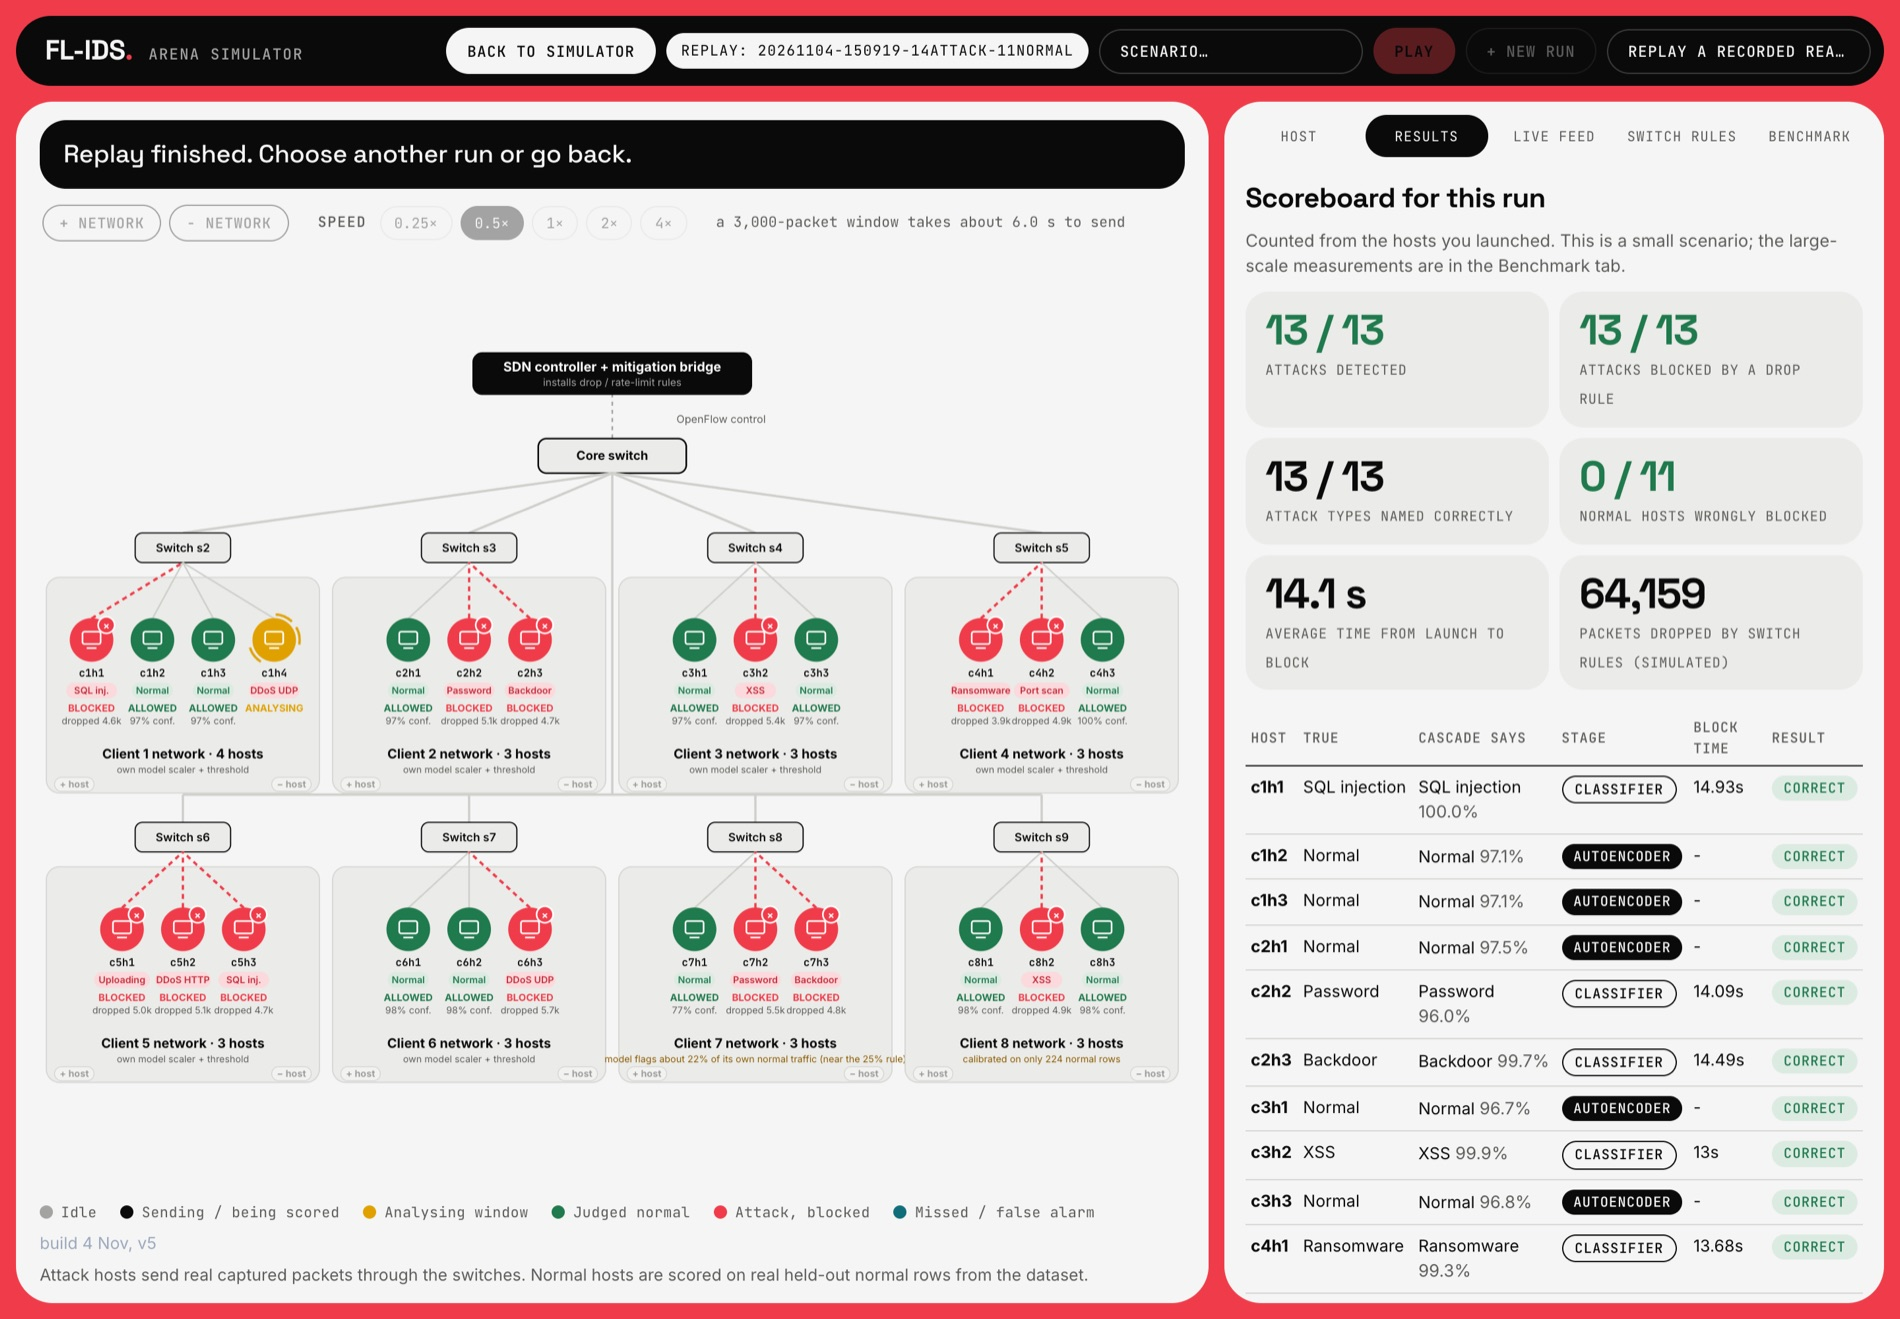
\includegraphics[width=0.84\linewidth]{figures/snap_arena_replay.jpg}
\caption{Replay of a recorded real run from the live lab (eight client networks, one with four hosts, 25 hosts in all). The scoreboard at the end of the replay shows 13 of 13 attacks detected, blocked and named correctly, 0 of 11 normal hosts blocked, 64,159 packets dropped and an average time to block of 14.1~s, because real packets were sent at 500 packets per second. Host c1h4 is still shown as analysing when the replay stops.}
\label{fig:snap:replay}
\end{figure}

\subsection*{Snapshots of malicious clients}
\begin{figure}[H]
\centering
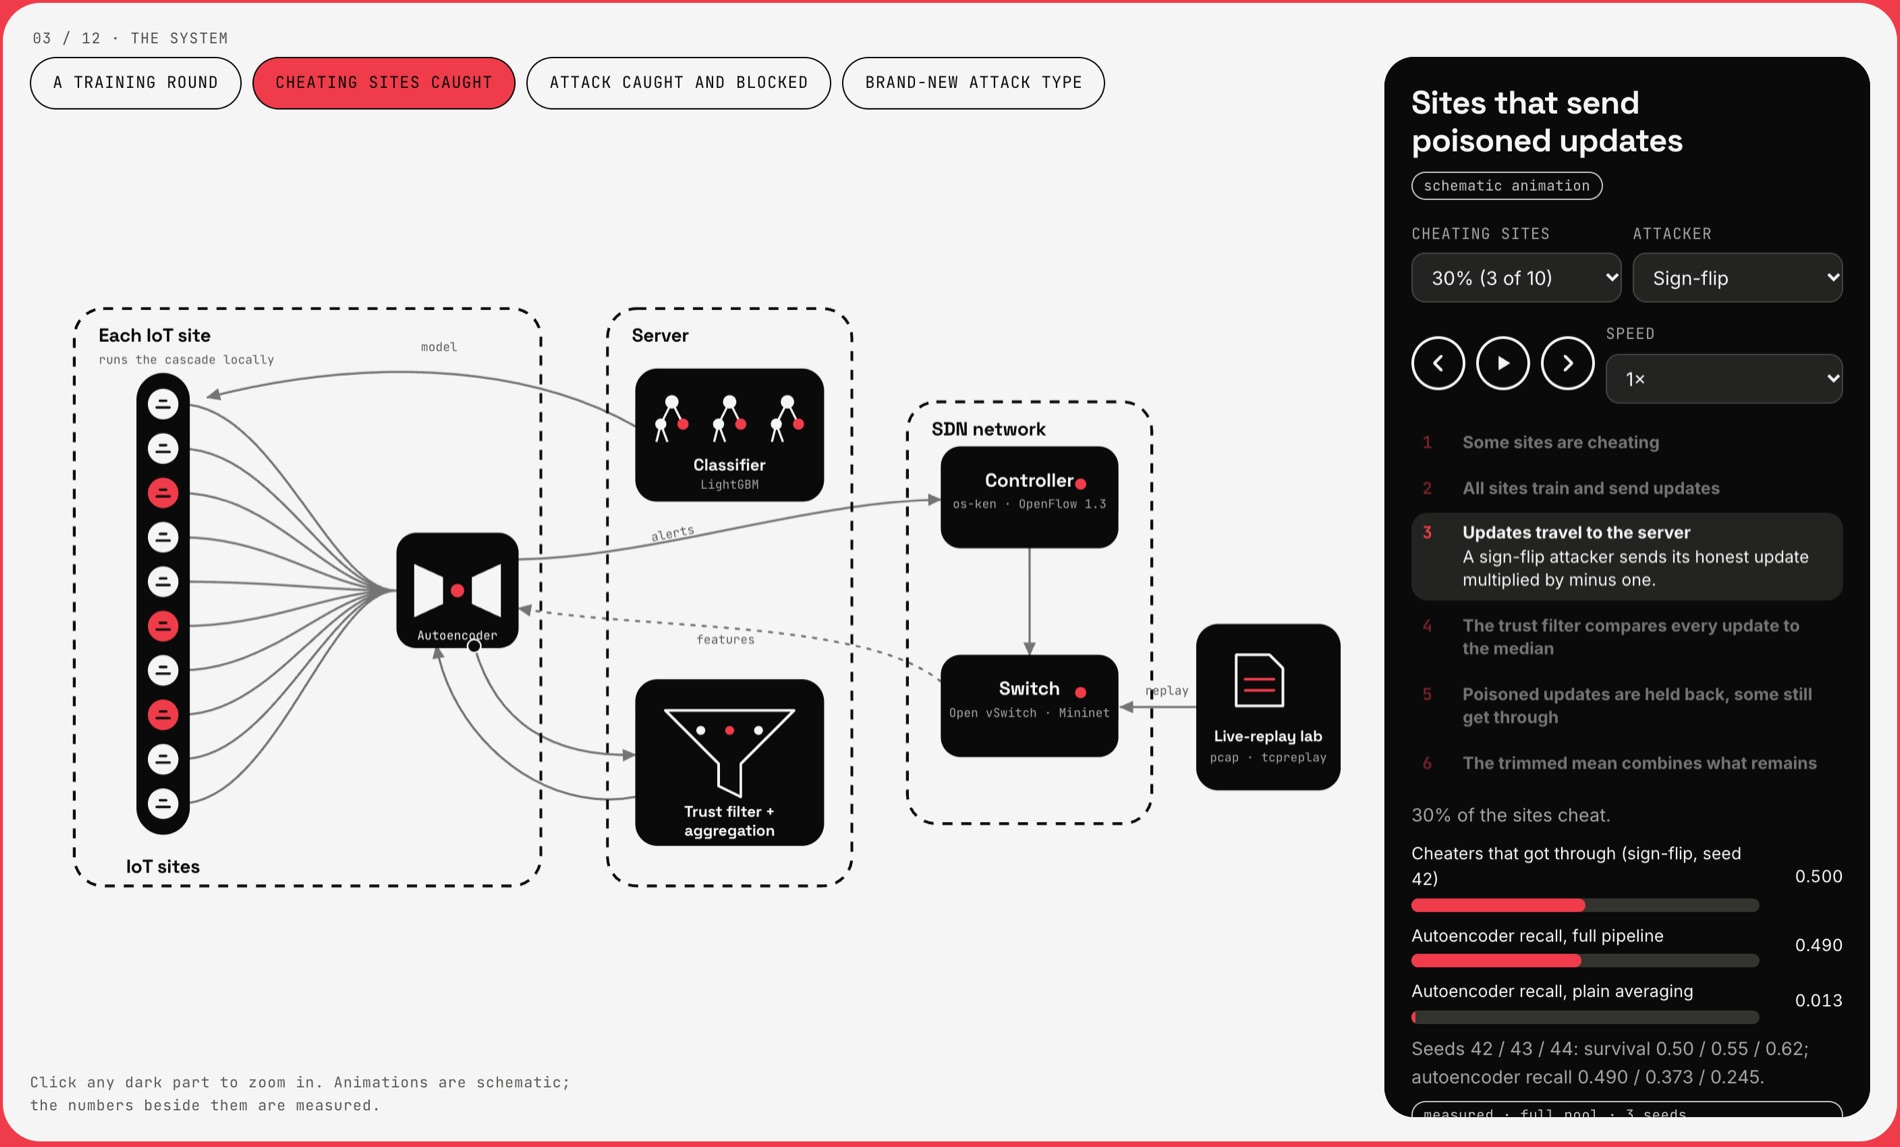
\includegraphics[width=0.84\linewidth]{figures/snap_cheat30.jpg}
\caption{Showcase site, scenario ``Cheating sites caught'': three of ten sites (red) send sign-flipped updates. The side panel gives the measured values for seed~42: half of the cheaters get past the trust filter (survival 0.500), the autoencoder recall of the full pipeline is 0.490 against 0.013 with plain averaging, and over seeds 42, 43 and 44 the survival is 0.50, 0.55 and 0.62. The animation is schematic; the numbers are measured.}
\label{fig:snap:cheat}
\end{figure}

\noindent The measured effect of malicious clients on the whole pipeline is given in Chapter~\ref{chap:results}, where the fraction of malicious clients is swept from 0\% to 50\% (the poisoning-resistance figure) and the per-round trust scores of honest and malicious clients are plotted.

\clearpage
\section {Appendix B: Details of list of publications related to this project}
{\large Author Names: } Aaron B Ajay, Aaryan Prakash, Amal Roy, Amogh Krishna JS, Syed Akram \\
{\large Paper Title: } Federated Learning-based Intrusion Detection System for SDN-enabled IoT Networks (working title) \\
{\large Name of the Conference or Journal:} Paper in preparation (draft in progress) \\
{\large Place of the conference:} -- \\
{\large Date of Conference:} --
\clearpage
\section {Appendix C: Details of Patent}
No patent has been filed for this work.
\clearpage
\section {Appendix D: Details of Funding}
This project did not receive external funding.
\clearpage
\section {Appendix E:POs and PSOs Mapped}
\begin{table}[h!]
\centering
\small
\renewcommand{\arraystretch}{1.05} % Row height
\setlength{\tabcolsep}{6pt}       % Column spacing
\begin{tabular}{|>{\raggedright\arraybackslash}p{3.6cm}|c|p{7.9cm}|}
\hline
\textbf{PROGRAMME OUTCOMES} & \textbf{Level (1/2/3)} & \textbf{Justification if addressed} \\
\hline
PO1 (Engineering knowledge) & 3 & Applies mathematics (cosine similarity, robust statistics, gradient boosting) and networking and machine-learning fundamentals to detecting attacks in IoT/IIoT traffic. \\
\hline
PO2 (Problem analysis) & 3 & Reviews the literature to identify gaps, and analyses why accuracy was stuck (content-free packets, ambiguity ceiling) and why aggregation fails under poisoning, with measured evidence. \\
\hline
PO3 (Design/development of solutions) & 3 & Designs a two-stage cascade, a trust-filtered federated aggregation scheme and an SDN mitigation path; keeps raw traffic on each site for privacy, which protects the safety of critical infrastructure. \\
\hline
PO4 (Conduct investigations) & 3 & Designs controlled experiments (ablation, poisoning sweep, zero-day tests, flow-grouped and multi-seed evaluation) and interprets the data to reach valid conclusions. \\
\hline
PO5 (Modern tool usage) & 3 & Uses LightGBM, PyTorch, Flower, Mininet, Open vSwitch, os-ken, TShark and Streamlit, and states each tool's limitations (for example, capture-level rather than inline mitigation). \\
\hline
PO6 (The engineer and society) & 2 & Addresses the security of IoT/IIoT systems society depends on, and the privacy concerns of sharing raw network traffic. \\
\hline
PO7 (Environment and sustainability) & 1 & Supports resilient, sustainable infrastructure (SDG 9); federated training avoids moving bulk traffic to a central site, and the system runs on existing hardware with open-source software. \\
\hline
PO8 (Ethics) & 3 & Keeps raw traffic on clients, uses a public dataset, reports dataset errors and limitations openly, and reports only numbers produced by logged runs. \\
\hline
PO9 (Individual and team work) & 3 & Developed by a four-member team, with each member owning components. \\
\hline
PO10 (Communication) & 2 & Documents the work in this report, a public repository with detailed notes, a results website, a presentation and a paper draft. \\
\hline
PO11 (Project management and finance) & 2 & Planned and delivered in phases with milestones tracked in version control, at zero cost using free and open-source software and existing hardware. \\
\hline
PO12 (Life-long learning) & 2 & Required independent learning of federated learning, adversarial robustness and SDN, which are beyond the regular curriculum. \\
\hline
\end{tabular}
\caption{Programme Outcomes Mapping with Project}
\end{table}

\begin{table}[h!]
\centering
\small
\renewcommand{\arraystretch}{1.05} % Row height
\setlength{\tabcolsep}{6pt}       % Column spacing
\begin{tabular}{|>{\raggedright\arraybackslash}p{3.6cm}|c|p{7.9cm}|}
\hline
\textbf{PROGRAMME SPECIFIC OUTCOMES} & \textbf{Level (1/2/3)} & \textbf{Justification if addressed} \\
\hline
PSO1 (Software engineering) & 3 & Applies software engineering practice: modular design by component, a single configuration file, 244 automated unit and integration tests, version control and reproducible, seeded runs. \\
\hline
PSO2 (Network, mobile and web-based systems) & 3 & Designs and builds a networked system under realistic constraints: a federated client--server system, an SDN-controlled emulated network, and a web dashboard, all running within the memory limits of a 4-vCPU virtual machine. \\
\hline
PSO3 (Efficient algorithms and code) & 3 & Designs efficient algorithms (trust filter on weight deltas, trimmed-mean aggregation, flow grouping of 2.2 million packets in about a minute) and effective code, such as one shared cascade implementation used by evaluation, dashboard and SDN. \\
\hline
\end{tabular}
\caption{Programme Specific Outcomes Mapping with Project}
\end{table}
\clearpage

\clearpage



\end{document}
